\documentclass[dissertation,CC-BY-ND]{uathesis}


\usepackage[a4paper,width=150mm,top=25mm,bottom=25mm]{geometry}
\usepackage[T1]{fontenc}
\usepackage[utf8]{inputenc}
\usepackage{authblk}
\usepackage{graphicx}
\usepackage{natbib}
%\usepackage{chapterbib}
\usepackage[cmex10]{amsmath}
\usepackage{amssymb}
\usepackage{amsthm}
\usepackage{mathrsfs}
\usepackage{hyphenat}
\usepackage{url}
\usepackage{listings}

\usepackage[bookmarks,colorlinks=true,urlcolor=black,linkcolor=black,citecolor=black]{hyperref}
\usepackage{cleveref}
\crefname{section}{Section}{Sections}
\crefname{figure}{Figure}{Figures}
\crefname{table}{Table}{Tables}
\setcounter{secnumdepth}{3} 
\setcounter{tocdepth}{3}

\newcommand{\Tmat}{\textbf{T}}
\newcommand{\vvec}{\textbf{v}}
\newcommand{\meanvvec}{\overline{\vvec}}
\newcommand{\delmeanvvec}{\Delta \meanvvec}
\newcommand{\vnhvec}{\boldsymbol{v_0}}
\newcommand{\vonevec}{\boldsymbol{v_1}}
\newcommand{\vtwovec}{\boldsymbol{v_2}}

\newcommand{\gvec}{\textbf{g}}
\newcommand{\meangvec}{\overline{\gvec}}
\newcommand{\delmeangvec}{\Delta \meangvec}
\newcommand{\gnhvec}{\boldsymbol{g_0}}
\newcommand{\gonevec}{\boldsymbol{g_1}}
\newcommand{\gtwovec}{\boldsymbol{g_2}}

\newcommand{\fvec}{\textbf{f}}
\newcommand{\xvec}{\textbf{x}}
\newcommand{\nvec}{\textbf{n}}
\newcommand{\rvec}{\textbf{r}}
\newcommand{\pvec}{\textbf{p}}
\newcommand{\Hmat}{\textbf{H}}
\newcommand{\Xvec}{\textbf{X}}
\newcommand{\Wvec}{\textbf{W}}

\newcommand{\Wv}{\textbf{W}_\textbf{v}}
\newcommand{\Wg}{\textbf{W}_\textbf{g}}
\newcommand{\WH}{\textbf{W}_\textbf{H}}

\newcommand{\Kv}{\textbf{K}_\textbf{v}}
\newcommand{\Kg}{\textbf{K}_\textbf{g}}
\newcommand{\Kx}{\textbf{K}_\textbf{x}}
\newcommand{\Kone}{\textbf{K}_\textbf{1}}
\newcommand{\Ktwo}{\textbf{K}_\textbf{2}}
\newcommand{\Kj}{\textbf{K}_\textbf{j}}

% Set up some values.
\completetitle{Development of a Three Sided Pyramid Wavefront Sensor for Astronomical Adaptive Optics}
\fullname{Lauren H Schatz}			% Grad college wants your full name here.
\degreename{Doctor of Philosophy}	% Title of your degree.

\begin{document}
\maketitlepage
{COLLEGE OF OPTICAL SCIENCES} % Title of your department.
{2020}	

\approval
{TB}		% Defense Date	
{Jared Males}	% 1st committee member
{Michael Hart}		% 2nd committee member
{tbd}
{tbd}

\statementbyauthor
% If this is a Thesis, use the following form, with your thesis director's
% name and title in the square brackets like so (you should also omit the 
% approval form insertion above):
%\statementbyauthor[Jane M. Doe\\Professor of Chemistry]

% Include the ``Acknowledgements''
\incacknowledgements{acknowledgements}

% Include the ``Dedication''
%\incdedication{dedication}

% Create a ``Table of Contents''
\tableofcontents

% Create a ``List of Figures''
\listoffigures

% Create a ``List of Tables''
\listoftables

% Include the ``Abstract''
\incabstract{abstract}

\chapter{Introduction}\label{CH1}

 
%% Introduce the problem and what we have to overcome to do it
%% last part need to detail all the things that is going in the dissertation nontechnical overview. 



\section{Exoplanets and the Habitable Zone}

 It is amazing that we have observed millions of objects in the universe, but have only detected a few thousand exoplanets. Exoplanets are planets in other star systems and as of February $24^{th}$, 2021 (the date the author started writing her dissertation!) there are 4,352 planets registered on the NASA exoplanet archive, (\cite{akeson2013nasa}). To put this into context we can compare the number of known exoplanets to other astronomical objects. In a recent Gaia survey, 1.3 million binary stars were cataloged by \cite{el2101million} The SIMBAD database currently details over 12 million objects varying from stars, galaxies, nebulae, supernovae, and more, (\cite{wenger2000simbad}). From this limited sample of exoplanet detections, we have discovered that other planetary systems look completely different from our own. The first exoplanet discovered around a sun-like star is 51 Pegasi b, a Jupiter-sized planet that has an orbit closer than Mercury's to its star, (\cite{mayor1995jupiter}). 

 Astronomers classify exoplanets in reference to our solar system. The categories are based upon exoplanet characteristics such as mass, radius, composition, and semi-major axis of the orbit. These classifications include but are not limited to: hot and cold Jupiters, Neptunes, terrestrial planets, and super-Earths. Figure \ref{fig:exoplanets} plots the known exoplanets as a function of mass and semi-major axis of the orbit. The mass is in units of Jupiter mass, and the semi-major axis is in units of AU. Almost all of the known exoplanets are larger than Earth, in the Neptune and Jupiter classes. This does not mean that Earth-like planets are rare, but that our current techniques of exoplanet detection are biased.

\begin{figure}
    \centering
    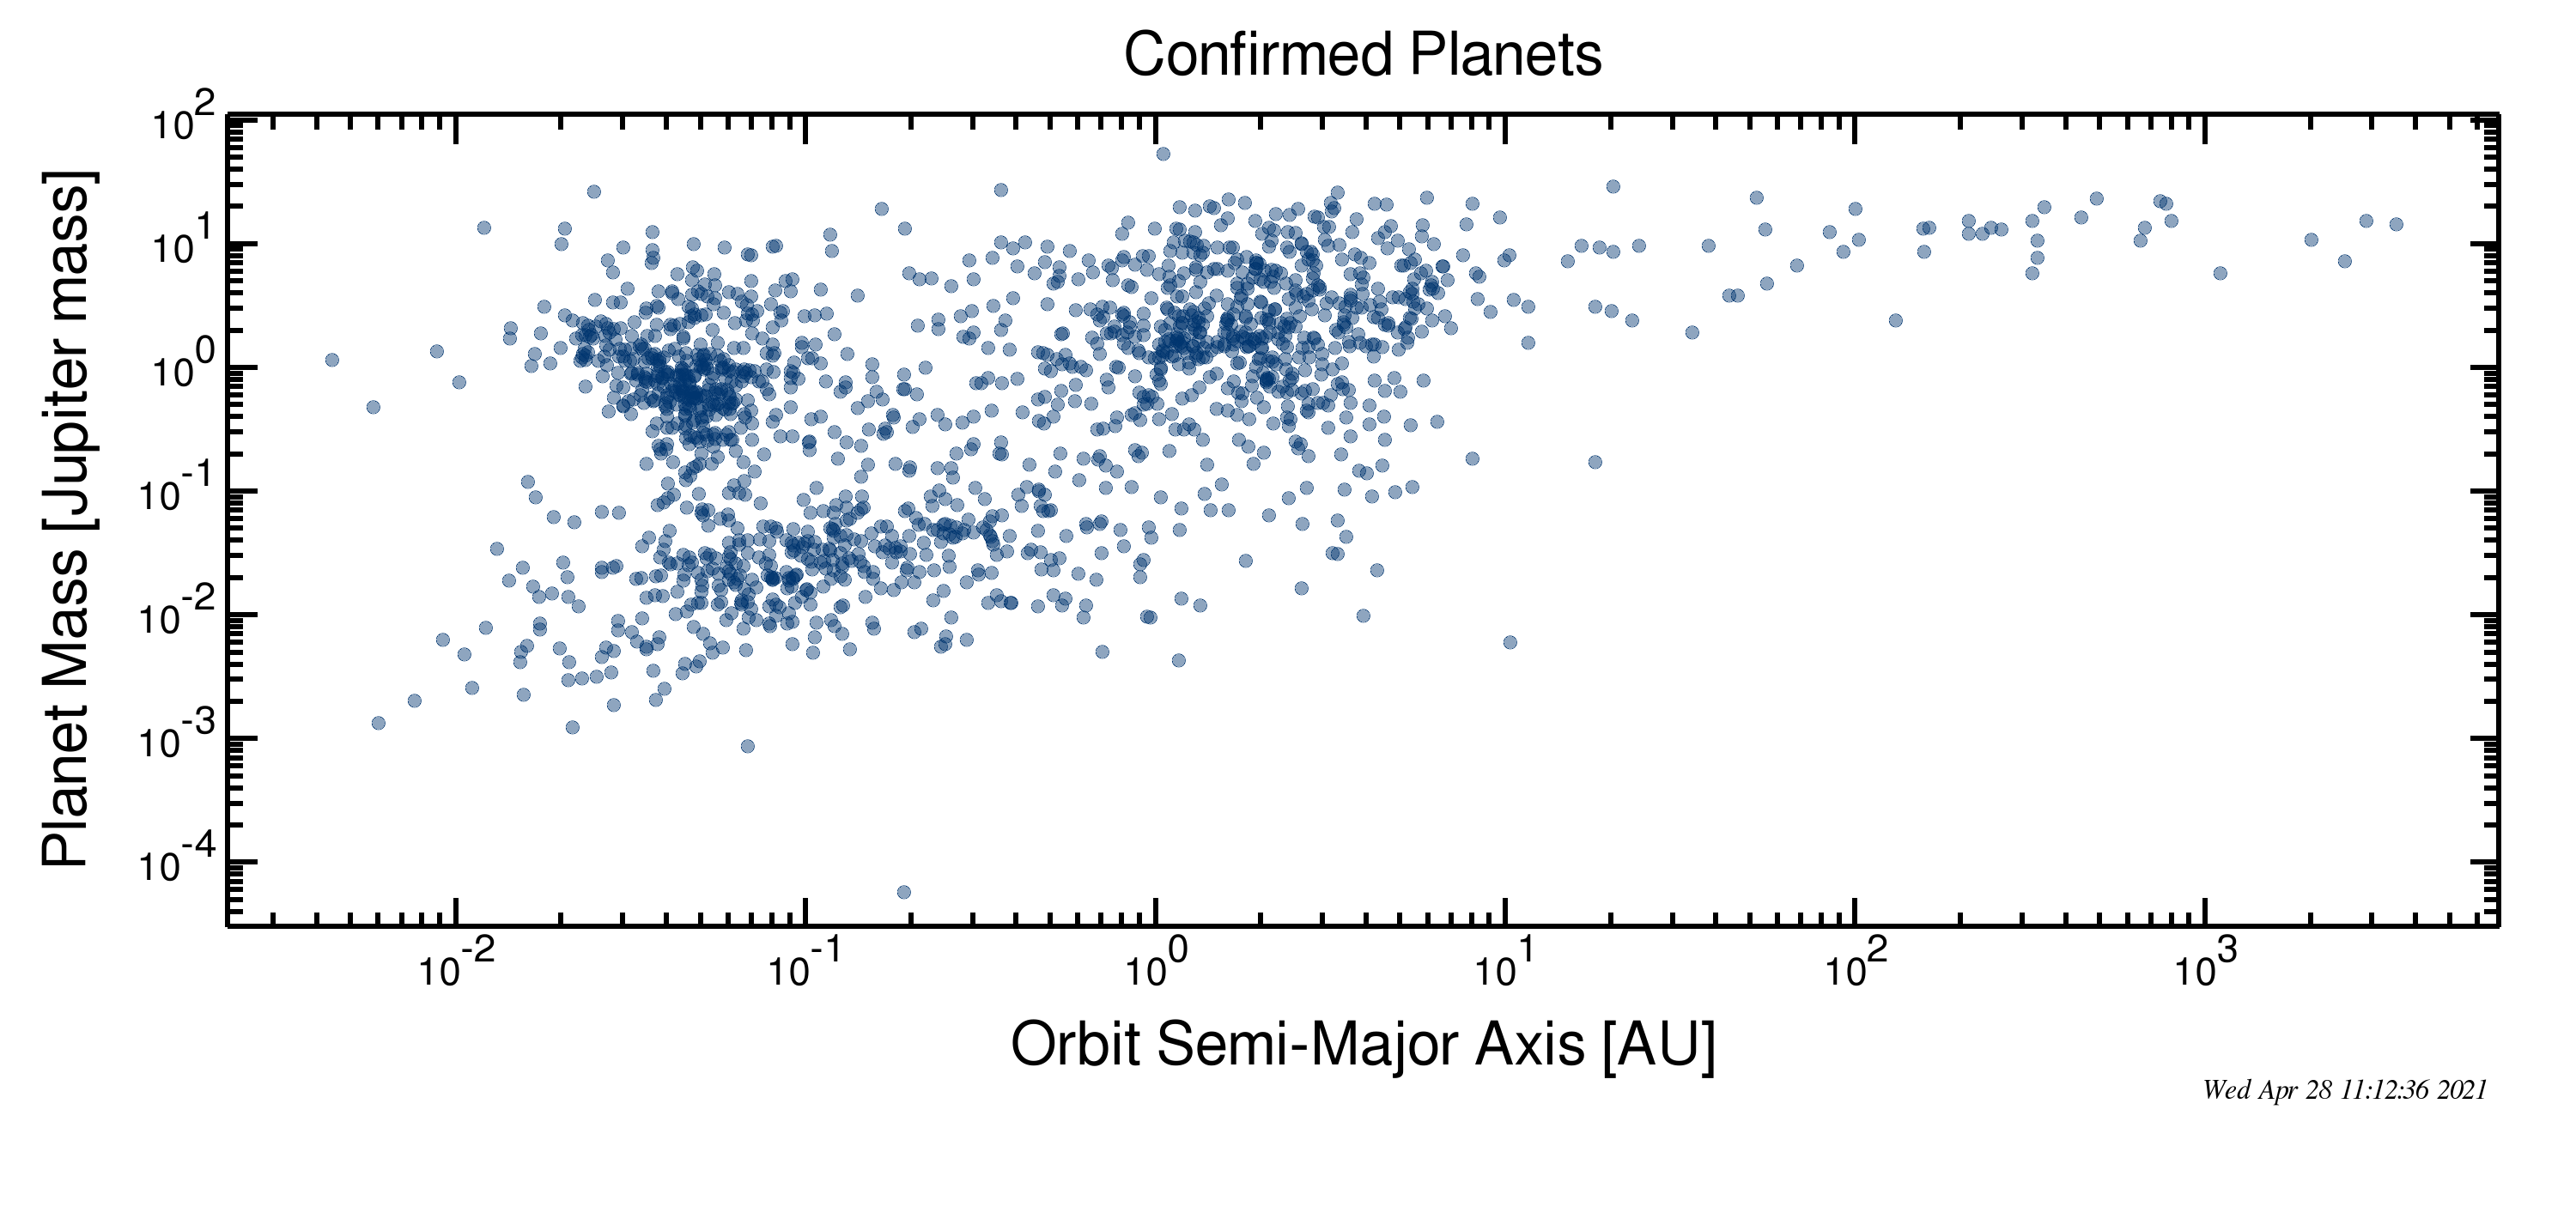
\includegraphics[width=0.8\textwidth]{Chapter Materials/Introduction Materials/MassVsSemiAxis.png}
    \caption{Plot of known exoplanets as a function of mass and semi-major axis. The plot was generated using tools and data provided by NASA exoplanet archive.}
    \label{fig:exoplanets}
\end{figure}

Two of the driving forces in exoplanet research are the detection and characterization of exoplanets. Different detection techniques favor different types of exoplanets and measure different characteristics. Studying these planetary systems can offer insight into the formation and evolution of our solar system. Of particular interest is the study of Earth-like planets orbiting in a region called the habitable zone. The habitable zone is defined as the region around a star where a terrestrial planet could support liquid water. The bounds of the habitable zone are determined by extremes. The inner edge is defined by the temperature where water escapes from the atmosphere due to a process called photolysis, the decomposition of molecules by light. The outer edge is defined by the formation of carbon monoxide clouds in the atmosphere. Carbon monoxide is a poor greenhouse gas and does not provide sufficient insulation for the planet to maintain liquid water, (\cite{seager2010exoplanets}). For our solar system, the Habitable zone is at 0.95-1.37AU. An estimate of the radius of the habitable zone can be found using equation \ref{HabitableZone}, and can be solved for our solar system by setting the temperature to T=300K, the luminosity to the solar luminosity L= 3.828×$10^{26}$W and solving for the radius of the orbit, r. The variable $\sigma_{SB}$ is the Stefan-Boltzmann constant. 



\begin{equation}
    \sigma_{SB}T^4=\frac{L}{4\pi r^2} 
    \label{HabitableZone}
\end{equation}



\section{Direct Imaging of Exoplanets}

 To study objects close to stars astronomers use a technique called direct imaging. In this method the exoplanet is resolved spatially from the star, allowing for a direct image of the planet to be taken as shown in Figure \ref{fig:exoplanets}, (\cite{bailey2013hd}). Direct imaging with astrometric calibration allows an astronomer to make precise measurements of the exoplanet’s period, and orbit, (\cite{seager2010exoplanets}). Using a series of narrowband filters we can measure the flux of the object at different wavelengths. This spectro-photometric characterization allows us to fit models of simulated atmospheres to estimate the composition and structure of the atmosphere,(\cite{morzinski2015magellan}). This includes features such as clouds and seasons, ( \cite{skemer2012first}). In combination with a spectrograph, we can start to directly characterize the composition of the exoplanet atmosphere by examining emission and absorption lines. 
 

\begin{figure}
    \centering
    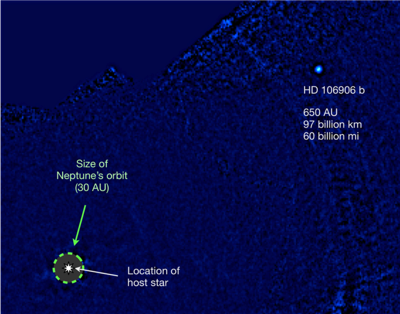
\includegraphics{Chapter Materials/Introduction Materials/Introduction Figures/HCexoplanet.png}
    \caption{Image of exoplanet HD 106906 b taken with the Magellan Adaptive Optics (MagAO) instrument. \cite{bailey2013hd}}
    \label{fig:exoplanets}
\end{figure}



\subsection{High Contrast Imaging}

High contrast imaging is a special case of direct imaging that is used to image faint companions next to bright stars. Targets include circumstellar disks, (\cite{rodigas2014morphology}), active galactic nuclei, (\cite{imanishi2020subaru}), and exoplanets, (\cite{bowler2016imaging}).Typically, exoplanets have flux contrasts of 10$^{-4}$ to 10$^{-10}$ with respect to their host stars. These high contrast ratios present challenges in directly imaging faint objects. Overcoming this contrast problem requires a two-fold solution. The starlight needs to be suppressed by a coronagraph, and the resulting high contrast region, called the dark hole, needs to be maintained over the course of the observation through extreme adaptive optics (ExAO) and wavefront sensing and control (WS$\&$C) techniques. ExAO systems operate by propagating light from a guide star to a wavefront sensor, which measures the phase error of the starlight wavefront. A computer then sends commands to shape a deformable mirror (DM) to correct for the phase error, forming a closed feedback loop that compensates for most of the atmospheric distortion. The corrected beam is then passed to a coronagraph which blocks the light from the on-axis star and allows us to detect faint off-axis sources. Figure \ref{fig:BetaCen} is a high contrast image of the binary star system $\beta$ Centauri using a vector apodizing phase plate coronagraph (vAPP), (\cite{snik2012vector}), on the Magellan Adaptive Optics System (MagAO), (\cite{close2018status}). There are many types of coronagraphs currently used in high contrast imaging; most work by blocking out light using masks and stops, (\cite{soummer2004apodized}), or using interferometric techniques to destructively interfere light at the focal plane,(\cite{foo2005optical}). Uncorrected phase errors and non-common path errors from the ExAO system result in speckles in the focal plane that reduce coronagraph contrast.
 

\begin{figure}
    \centering
    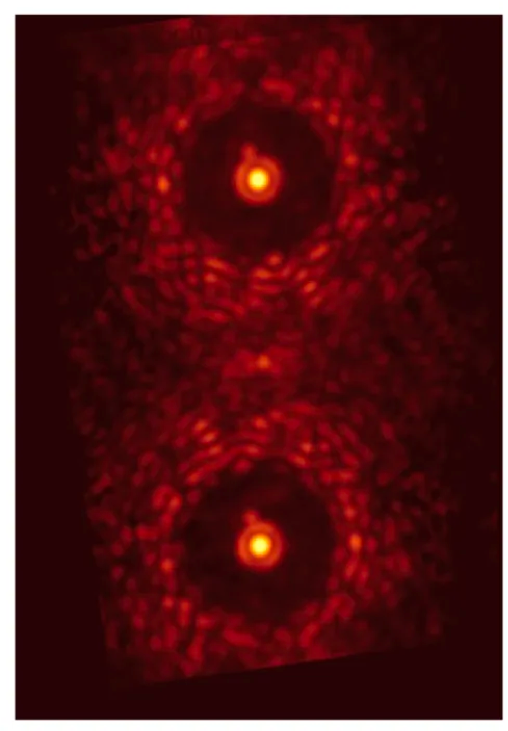
\includegraphics{Chapter Materials/Introduction Materials/BetaCen.png}
    \caption{High contrast image of star system $\beta$ Centauri using a vAPP coronagraph on MagAO. The vAPP creates two copies of the corongraph PSF in a single image. }
    \label{fig:BetaCen}
\end{figure}



\section{Exoplanet Imaging with Giant Segmented Mirror Telescopes}

Within the next decade, the world will see a new generation of Giant Segmented Mirror Telescopes (GSMTs). The Giant Magellan Telescope (GMT) under construction at Las Campanas Observatory, Chile, will have seven 8.4-meter mirrors, forming a 24.5-meter primary mirror, (\cite{fanson2020overview}.) The Thirty Meter Telescope (TMT), and the European Extremely Large Telescope(E-ELT) at Cerro Paranal, Chile, have highly segmented primary mirrors, (\cite{chisholm2020thirty}). The 39-meter E-ELT primary mirror will be comprised of hundreds of 1.4-meter hexagonal segments,(\cite{ramsay2020eso}). The TMT will have 492, 1.44-meter hexagonal segments to form the 30-meter primary mirror, (\cite{sanders2013thirty}). The GSMTs will have the light-collecting power to detect and characterize potentially habitable terrestrial exoplanets for the first time. This will only be achievable if the performance of GSMT-ExAO systems is optimized. Alternative architectures of wavefront sensors are under consideration for GSMT-ExAO instruments considering the trade-offs between detector size, speed, and noise that determine the performance of GSMT-ExAO wavefront control. 

 The GSMTs all plan to use pyramid wavefront sensors (PWFS) in ExAO instruments. The PWFS acts like a Foucault test in 2 dimensions. Light from the telescope is focused onto a glass pyramid tip where it is split and then the pupil plane is reimaged onto a detector. The result is copies of the telescope pupil that contain intensity fluctuations that are related to the wavefront phase. All current PWFS on telescopes use a four-sided pyramid (4PWFS), resulting in four pupil copies. The Planetary Systems Imager \cite{fitzgerald2019planetary} for the TMT will use a non-modulated PWFS\cite{guyon2018wavefront} in combination with lower order wavefront control to reach and maintain high contrast. The Multi-AO Imaging Camera for Deep Observations (MICADO)\cite{davies2018micado} for the E-ELT is a pathfinder instrument for performing high contrast imaging on GSMTs that uses a PWFS. The High Angular Resolution Monolithic Optical and Near-infrared Integral field spectrograph (HARMONI)\cite{neichel2016adaptive}, also for the E-ELT has a PWFS in the single conjugate adaptive optics (SCAO) mode to deliver diffraction limited performance for the E-ELT's core spectroscopic capability. The Giant Magellan Extreme Adaptive Optics System (GMagAO-X)\cite{males2019gmagao} is being developed as a first light ExAO instrument for the GMT and will use a PWFS.


This dissertation aims to develop the three-sided pyramid wavefront sensor (3PWFS) as an alternative GSMT-ExAO wavefront sensor. The 3PWFS  uses fewer detector pixels so it is less sensitive to read noise than the 4PWFS. In Chapter \ref{CH1}, we determine the expected signal from a telescope and detail how atmospheric turbulence degrades image quality. Chapter \ref{CH2} describes the pyramid wavefront sensor and a mathematical formalism based on the diffraction theory description of the Foucault knife-edge test that predicts the intensity pattern after the PWFS. Our formalism allows us to calculate the intensity in the pupil images formed by the PWFS in the presence of phase errors corresponding to arbitrary Fourier modes. We use these results to motivate how we process signals from a 3PWFS. We compare the Raw Intensity method which uses the signal in the pupils as is, and derive the Slopes Maps calculation for the 3PWFS which combines the three pupil images of the 3PWFS to obtain the X and Y slopes of the wavefront. In Chapter \ref{CH3} we describe the design and current status of the MagAO-X 4PWFS. We then use the Object Oriented MATLAB Adaptive Optics toolbox (OOMAO) in Chapter \ref{Ch4} to simulate an end-to-end model of an adaptive optics system using a PWFS with modulation and compare the performance of the 3PWFS to the 4PWFS. In Chapter \ref{CH5} we present the Comprehensive Adaptive Optics and Coronagraph Test Instrument (CACTI), which was designed with the flexibility to support visiting instruments and to be easily re-configurable to perform multiple experiments. We first describe the design of CACTI, review its operation and calibration procedures, and discuss its current status. We then discuss an experiment performed on CACTI with a visiting three-sided pyramid wavefront sensor (3PWFS) to explore an alternative wavefront sensor architecture for GSMT-ExAO. Both a 3PWFS and 4PWFS were integrated into  CACTI to demonstrate the operation of a 3PWFS and compare it to the 4PWFS. We present results from experiments demonstrating the operation of the 3PWFS, and comparisons to the 4PWFS. Finally, in Chapter \ref{CH6}, we discuss the conclusions we can draw from the outcome of these experiments.



% Exoplanet signals are small, and need long exposures to overcome photon noise. Astronomers co-add images to beat down the noise, sometimes data across multiple nights are used in a single exoplanet detection. 

%% Habitable zone
% direct imaging
% high contrast imaging
% this is the problem
% here is our solution

%% Chapter two technical background







%\bibliographystyle{IEEEtranS}  
%\bibliography{ThesisBib}


% The search for life and habitable words beyond our solar system is a driving force of modern astronomy and one of the most captivating questions of our time.
\chapter{Analysis of the PWFS Signals}\label{CH2}
%Babcock. Summary of some on sky systems. 

A key component of an ExAO system is the WFS, which measures aberrations from atmospheric turbulence.  A common choice in current and next generation instruments is the pyramid wavefront sensor (PWFS). The PWFS is a highly sensitive wavefront sensor that is able to measure the wavefront at high speed. The sensitivity and linear range of the PWFS can be tuned by dynamic modulation, making the PWFS robust to different seeing conditions. 
\section{The Pyramid Wavefront Sensor} 
The optical design of the PWFS consists of four components: a focusing optic, the glass pyramid, and a relay lens to image the pupils on the detector.\cite{ragazzoni2002pyramid} Figure \ref{fig:pyramid} shows a schematic of the operation of a PWFS.  The starlight is first brought to a focus on the tip of a glass pyramid that splits the focal plane into parts. The apex angle of the pyramid imparts a tilt to separate each of the sections. The result is copies of the telescope pupil that are separated spatially on a detector. The number of pixels across each pupil determines the number of modes the instrument is sensitive to. Current on-sky adaptive optics systems that have a PWFS use a four-sided PWFS. The Magellan Adaptive Optics System (MagAO)\cite{close2018status}, the Large Binocular Telescope Interferometer (LBTI)\cite{esposito2011adaptive}, and MagAO-X use an achromatic double four-sided pyramid. The SCExAO instrument uses two crossed roof prisms as its pyramid optic. The PWFS is highly sensitive but suffers from low dynamic range. A modulator is used to increase the linear range of the PWFS. Modulation is achieved by oscillating a piezo-actuator driven mirror to drive the PSF on the pyramid tip into a circular pattern with a radius quoted in units of $\lambda/D$, where $\lambda$ is wavelength, and $D$ is the diameter of the entrance pupil. This increases the effective spot size on the pyramid tip which increases the sensor's linearity at the cost of sensitivity.\cite{guyon2005}  

\begin{figure}
    \centering
    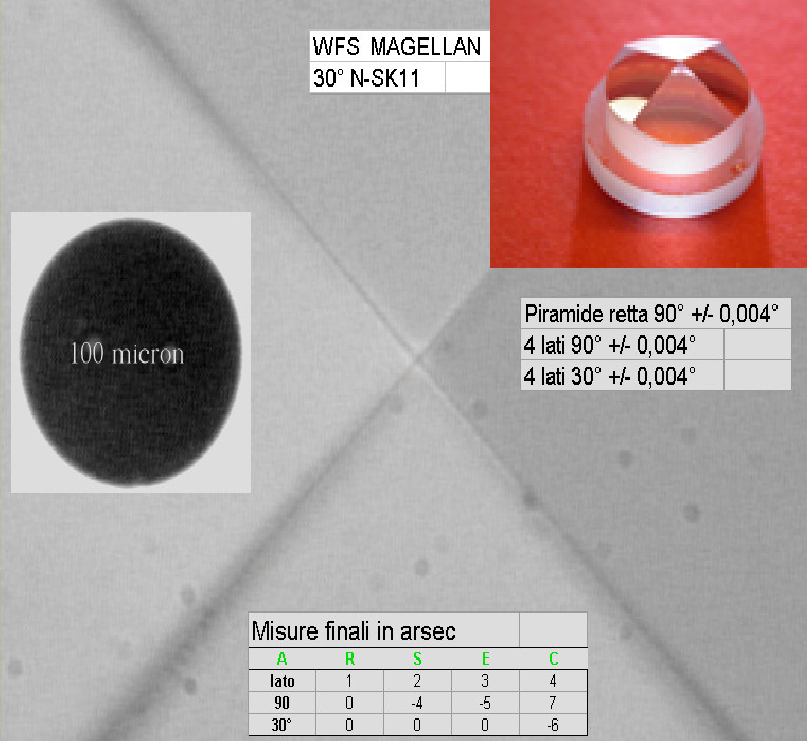
\includegraphics[width=0.75\textwidth]{Chapter Materials/Chapter Three Materials/pyramid.png}
    \caption{Optical design of a PWFS. Light from the telescope is focused onto a glass pyramid tip where it is split and then the pupil plane is reimaged onto a detector. The result is copies of the telescope pupil that contain intensity fluctuations that are related to the wavefront phase. \cite{pyramidfig}}
    \label{fig:pyramid}
\end{figure}


The intensity measured in the PWFS must be processed to infer the wavefront phase. First, the image is dark subtracted and gain corrected to remove detector artifacts. A threshold mask is then applied to mask out any pixels that do not contain a signal. The wavefront sensor response to a flat wavefront is subtracted off to leave only the intensity pattern caused by the wavefront phase error. The intensity in the pupils can be combined to estimate the wavefront derivative, or slope. We refer to this as the Slopes Maps (SM) calculation. The equation for the 4PWFS is,


\begin{eqnarray}
    S_x=\frac{I_1+I_2-I_3-I_4}{I_1+I_2+I_3+I_4}     \label{4PWFSslopes} \\
    S_y=\frac{I_1-I_2-I_3+I_4}{I_1+I_2+I_3+I_4} \nonumber
\end{eqnarray}

where $S_x, S_y$ are the local wavefront slopes in the x and y direction, and $I_1...I_4$ are the intensity values of the pixel corresponding to the same location in each pupil. The intensity patterns in the pyramid pupils contain both the X and Y spatial information of wavefront gradient from the diffraction off of the pyramid edges. The Raw Intensity (RI) signal processing method uses the pyramid signal as-is. The benefit of the Raw Intensity method is that it is relatively unaffected by alignment errors. The major challenge in using this technique is obtaining a good flat wavefront reference image. The signals in the pyramid pupils are then extracted into a single column vector of intensity values.

All current PWFSs on telescopes use a 4PWFS. ExAO systems need high sampling of the PWFS pupils to optimize performance, and as a result require larger detectors. Detector size, speed, and noise all impose limits on wavefront sensor designs and limit the performance of an GSMT-ExAO system. We are interested in exploring the 3PWFS as an alternative PWFS for an ELT-ExAO wavefront sensor to overcome these limitations. The 3PWFS only has three copies of the pupil and therefore uses fewer detector pixels than the 4PWFS and should be less sensitive to read noise. We assess the performance of the 3PWFS compared to the 4PWFS in simulation to determine if the 3PWFS does outperform the 4PWFS when using high read noise detectors.

To assess the performance of the 3PWFS compared to the 4PWFS, a simulation was developed using the Object Oriented Matlab Adaptive Optics toolkit (OOMAO) \cite{OOMAO}. The OOMAO toolkit is an end-to-end adaptive optics model that can simulate different combinations of guide stars, turbulent atmospheres, wavefront sensors, deformable mirrors, and science cameras. Light is propagated using Fraunhofer diffraction. The PWFS is simulated using a single tip/tilt phase mask that is segmented into N parts. Figure \ref{fig:oomaoFigs}.A and \ref{fig:oomaoFigs}.C show the masks for the 3PWFS and 4PWFS. The masks are scaled and rotated according to a user input for rotation and pyramid apex angle that controls the separation of the pyramid pupils. After scaling, the mask is converted into a phase mask that is applied at the focal plane to simulate a pyramid tip. Figure \ref{fig:oomaoFigs}.C and \ref{fig:oomaoFigs}.D show the resulting pyramid pupils on the simulated wavefront sensor camera, using a flat wavefront and 5 $\lambda/D$ modulation. The master OOMAO toolbox simulates a 4PWFS using Slopes Maps. We extended the PWFS class in OOMAO to include a 3PWFS, taking care that the amplitude of the tip/tilt phase in the 3PWFS phase screen generation matched that of 4PWFS. We included our derivation of the Slopes Maps equation for the 3PWFS (derived in Section~\ref{SlopesDerivation} below), and added the Raw Intensity method for both the 4PWFS and the 3PWFS. For both the Slopes Maps and Raw Intensity method the signal was normalized by the mean value across all valid pixels on the wavefront sensor detector, instead of normalizing pixel by pixel. 

\begin{figure}
    \centering
    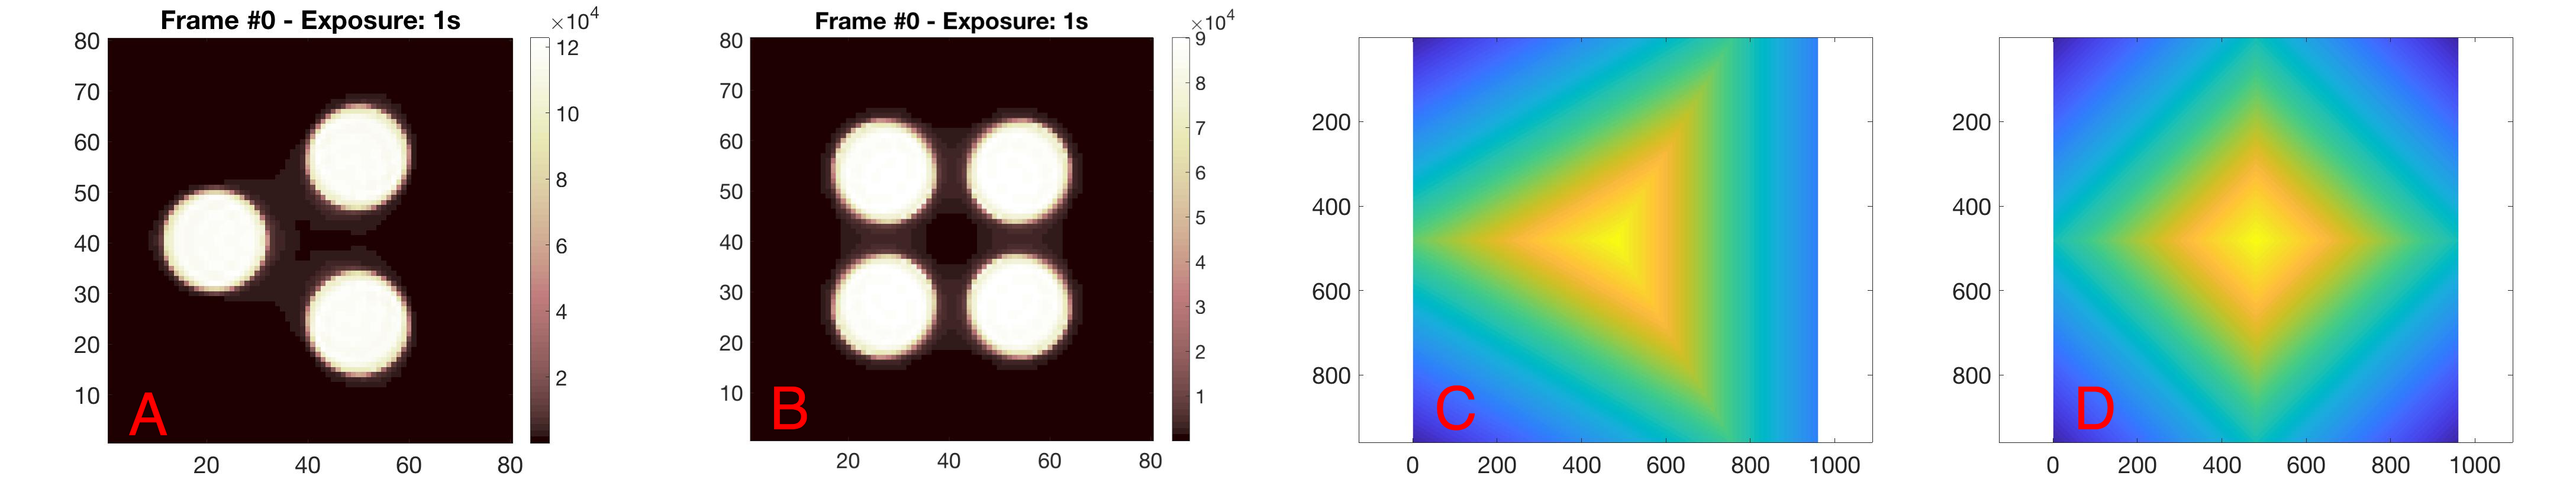
\includegraphics[width=1\textwidth]{Chapter Materials/Chapter Two Materials/oomaoFigs.png}
    \caption{Details of the simulated PWFS in OOMAO. A) and B) The simulated 3PWFS and 4PWFS pyramid masks in OOMAO. These masks are used as a phase screen in the pupil plane to emulate the focal plane splitting and separation done by a real glass pyramid. C) and D) The pupils from the 3PWFS and 4PWFS respectively on the simulated detector. In OOMAO the user can change the size, separation, and intensity values of the pupils through user defined inputs.}
    \label{fig:oomaoFigs}
\end{figure}


\section{Diffraction Theory of the Foucault Test}\label{diffraction}
\subsection{Derivation of Expected Signal from the Foucault Test}
  The PWFS is an extension of the knife edge test: each of the pyramid pupils are the signal from a knife edge test, but include a mirroring effect of the signal across the facets. The underlying physical processes of the pyramid and the knife edge are the same, so we can use the equations that describe the knife edge test explore the operation of the PWFS. The diffraction theory of the PWFS has been studied in detail. Vérinaud\cite{verinaud2004nature} extends the knife edge diffraction theory to model the signal of a roof sensor with dynamic circular modulation. Hutterer et. al.\cite{hutterer2019real} extends the knife edge analysis into general operators such that modulations of any pattern can be modeled. Shatokhina et. al.\cite{shatokhina2014fast} presents simplified equations to approximate pyramid signals with and without modulation. Correia et. al.\cite{correia2020performance}, and Fauvarque et. al.\cite{fauvarque2019kernel} model the pyramid operation as a Fourier filter. In this paper we use a formalism similar to Vérinaud, but limit our analysis to that of a one dimensional knife edge test for simplicity. We use the knife edge analysis to derive the relationship of the PWFS sensitivity to Fourier modes. Fourier modes have a direct relationship to locations on the focal plane; which is important to coronagraphy because we are trying to maximize the contrast in the dark hole region created by the coronagraph.
 
 In this section we consolidate the diffraction theory of the knife edge test by Linfoot\cite{linfoot1948theory}, Katzoff\cite{katzoff1971quantitative}, and Wilson\cite{wilson1975wavefront} into a single derivation with uniform notation. Expanding upon their results, we link phase aberrations in the shape of Fourier modes to intensity patterns produced by the knife edge test. We assume a focal plane bisected by a binary amplitude mask representing the knife edge. 
 
 Figure \ref{fig:derivationFlow} describes the steps taken in this derivation. The diagram is in two dimensions for visualization, but in this derivation we assume a one dimensional case for simplicity. We start with an electric field in the entrance pupil, $u_0(x_0)$ that has a phase error given by $\cos(nx)$. A Fourier transform is taken to the focal plane where the knife edge, $H_f(\xi_f)$ is applied. We don't actually solve for $U(\xi_f)$, the electric field in the focal plane, and instead take an inverse Fourier transform to the conjugate pupil plane where the knife edge test signal is found. The electric field at this pupil plane is given by $u(x_i)$, is the convolution of the electric field in the entrance pupil propagated to this pupil plane, $u_0(x_i)$, and the inverse Fourier transform of the knife edge, $h_i(x_i)$. The phase error in the electric field is expanded in a power series, then linearized, and the modulus squared is taken to find the field intensity. By subtracting off the constant term, we are left with the intensity pattern due to only the phase errors. 
 
 
 
 \begin{figure}
     \centering
     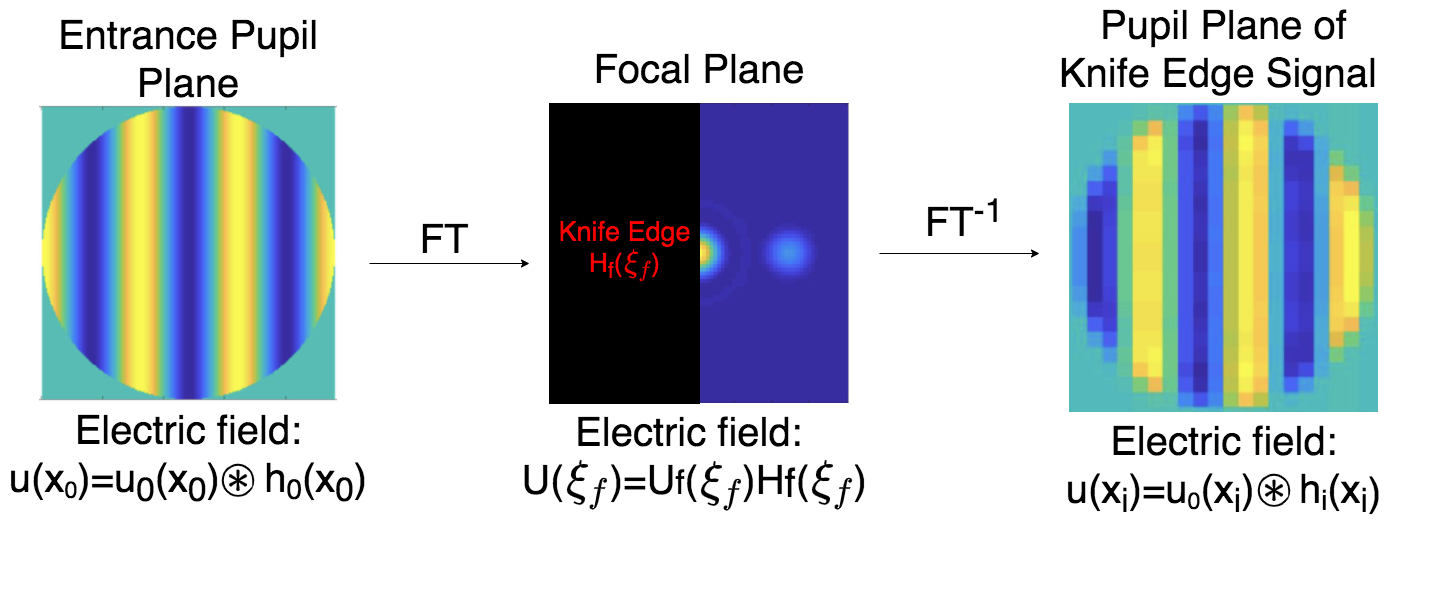
\includegraphics[width=0.9\textwidth]{Chapter Materials/Chapter Two Materials/DerivationFlow.png}
     \caption{Diagram of the steps taken in the derivation. The entrance pupil with electric field $u_0(x_0)$ is Fourier transformed to the focal plane. At the focal plane the knife edge by multiplying the binary mask function of the knife edge, $H_f(\xi_f)$, by the Fourier transform of the electric field in the entrance pupil. An inverse Fourier transform taken to return to the pupil plane where the pyramid signal is detected.}
     \label{fig:derivationFlow}
 \end{figure}
 
 


% To start, we define some terms used in the derivation. 

% \begin{center}
%     \begin{tabular}{ | l |p{12cm}|}
%     \hline
%     $u_0(x_0)$ & Complex wavefront at the "phase object". This could be the surface of a mirror under testing, but for our application it is the phase errors in the pupil caused by atmospheric turbulence. \\ \hline
%     $u_i(x_i)$ & Complex wavefront at the image plane. For the pyrmaid wavefront sensor the image plane is the pupil plane. \\ \hline
%     $h(x_i)$ & The impulse response of the system. \\ \hline
%     $m(x)$ & The equation of phase error to be measured. $u(x)=exp(-2\pi i m(x))$  \\ \hline
%     $p(x_i )$ & The intensity pattern at the image plane due to the diffraction of the electric field with the knife-edge \\ \hline
%     \end{tabular}
% \end{center}

To start we define the electric field in the entrance pupil as $u_0(x_0)$. We take the Fourier transform the of the electric field to get to the focal plane, where we will apply the knife-edge. The Fourier transform is here defined as,

\begin{equation}
    \mathcal{F}\{\xi_x\}=\frac{1}{2\pi}\int_{-\infty}^\infty e^{-i x \xi_x} f(x) dx
    \label{FourierT}
\end{equation}

where $\xi_x$ is the spatial frequency corresponding to the spatial coordinate $x$. $\mathcal{F}\{\cdot\}$ denotes the Fourier transform operator, and  $\mathcal{F}^{-1}\{\cdot\}$ will denote its inverse. The equation of the electric field in the focal plane, $U(\xi_f)$ is:

\begin{equation}
    U (\xi_f)=U_f(\xi_f)H_f(\xi_f)
    \label{FT}
\end{equation}

where,
% We now multiply the transmission function of the knife edge, $H(\xi_x)$. In this derivation we assume that the knife edge is like a step function, the transmission of light is 1 until the edge of the knife edge is reached and then drops to zero. We assume for simplicity that the aperture is infinite, but that the knife edge eclipses half of it. After multiplication, the Fourier transform of equation must be taken again to calculate the electric field in the pupil plane. We write out the step function in terms of the sign function $sgn(\xi_x)$, in order to calculate the Fourier Transform easily. The transfer function of the knife edge is given by the following equation.
\[ 
H_f(\xi_f)= 1/2+1/2\mbox{sgn}(\xi_f) \left\{
\begin{array}{ll}
      1 \: for \: \xi_f >0\\
      0 \: for \: \xi_f <0\\
      
\end{array} 
\right. 
\]

is the binary mask function of the knife edge, and $U_f(\xi_f)$ is the Fourier transform of $u_0(x_0)$. Taking the inverse Fourier transform brings us to the conjugate pupil plane. The inverse Fourier transform of $H_f(\xi_f)$ is

% \begin{equation}
%      FT^{-1}[H(\xi_x)]=\frac{1}{2\pi}\int_{-\infty}^\infty e^{ i x \xi_x} ( \frac{1}{2}+\frac{1}{2}sgn(\xi_x)) d\xi_x \\
%  =\frac{1}{2}\delta(-x)+\frac{i}{2\pi}(\frac{1}{x})
% \label{delta}
% \end{equation}

\begin{equation}
    h_i(x_i)= \mathcal{F}^{-1}[H_f(\xi_f)] =
    % \frac{1}{2\pi} \int_{-\infty}^\infty e^{ i x \xi_f}
    % \left(
    %     \frac{1}{2} + \frac{1}{2} \mathrm{sgn}(\xi_f)
    % \right) d\xi_f
    % = 
    \frac{1}{2} \delta(-x_i) + \frac{i}{2\pi} \left(\frac{1}{x_i}\right)
\label{delta}
\end{equation}


%  = \frac{1}{2} \frac{1}{2\pi} \int_{-\infty}^\infty e^{- i x \xi_x}d\xi_x+\frac{1}{2} \frac{1}{2\pi}\int_{-\infty}^\infty e^{- i x \xi_x}sgn(\xi_x) d\xi_x
% \end{align*}

% We make use of the property of the delta function to solve for the Fourier Transform of $\frac{1}{2}$:

% \begin{equation}
%     \delta(x)=\frac{1}{2\pi}\int_{-\infty}^\infty e^{ i x \xi_x}d\xi_x
% \end{equation}

% which leads to,
    
% \begin{equation}
%     \frac{1}{2}\delta(x)=\frac{1}{2}\frac{1}{2\pi}\int_{-\infty}^\infty e^{ i x \xi_x}d\xi_x 
% \end{equation}

% where $\frac{1}{2}\delta(x)$ is the Fourier Transform of $\frac{1}{2}$. To solve for the Fourier transform of $\frac{1}{2} sgn(\xi_x)$ function, we use the derivative property.

% \begin{equation}
%   FT[\frac{d g(x)}{dx}]=i2\pi \xi_x G(\xi_x)
%   \label{derivativeProp}
% \end{equation}

% where the derivative of $\frac{1}{2} sgn(\xi_x)$ is $\delta(\xi_x)$. Plugging this into Equation~\ref{derivativeProp}, gives the result,
% \begin{equation}
%   FT[\frac{d sgn(\xi_x)}{d\xi_x}]=FT[\delta{\xi_x}]=1=2\pi i x G(x).
% \end{equation}

% Solving for $G(x)$,
% \begin{equation}
%  G(x)=\frac{1}{i2\pi x}.
% \end{equation}

% Now we can sum our answers to get the Fourier Transform of a step function.

% \begin{equation}
%  FT[step(\xi_x)]=\frac{1}{i2\pi x_i}+\frac{1}{2}\delta(x_i)
%  \label{knifeedge}
% \end{equation}

We take the results of Equation~\ref{delta} and convolve it with $u_0(x_i)$, which is the Fourier transform of $U_f(\xi_f)$ in Equation~\ref{FT}, to get the electric field at the pupil plane, $u(x_i)$. The resulting equation is Equation 5a from Wilson.\cite{wilson1975wavefront}


% \begin{equation}
%   u_i(x_i)= u_0(x_0) \circledast \frac{i}{2\pi x_i}+\frac{1}{2}\delta(-x_i) 
%  = \int_{-\infty}^\infty u_0(x')[\frac{1}{2}\delta(x'-x_i)+\frac{i}{2\pi}\frac{1}{x_i-x'}]dx' 
% \end{equation}
%  \begin{equation}
%       u_i(x_i) =\frac{1}{2}u_0(x_i)+\frac{i}{2\pi}\int_{-\infty}^\infty \frac{u_0(x')dx'}{x_i-x'}
%       \label{KEconv}
%  \end{equation}

\begin{equation}
    u(x_i)= u_0(x_i) \circledast \left(
        \frac{i}{2\pi x_i}+\frac{1}{2}\delta(-x_i)
    \right)
    =
    \int_{-\infty}^\infty
    u_0(x') \left[
        \frac{1}{2}\delta(x'-x_i)+\frac{i}{2\pi}\frac{1}{x_i-x'}
    \right] dx' 
    \label{KEconv}
\end{equation}

The first modification to Equation~\ref{KEconv} by Wilson and Katzoff is to assume that the pupil has a finite aperture, resulting in the integral limits of -1 to 1. The following equations are equations 6 through 9 in Wilson's paper.\cite{wilson1975wavefront} For a perfect wavefront we assume $u_0 (x_i )=1$.  Wilson and Katzoff define $m(x)$ as the local mirror error in half-wavelengths, but for our application it would be the phase errors caused by atmospheric turbulence. Assuming an electric field with some phase error $m(x)$ we first expand the electric field as a Taylor series as follows,
\begin{equation}
    u_0 (x_i )=e^{(-2\pi i m(x_i ))}=1-2\pi i m(x_i )-2\pi^2*m^2 (x_i )+...
    \label{taylorexp}
\end{equation}
and disregard all higher order terms. Substituting Equation~\ref{taylorexp} into Equation~\ref{KEconv} and simplifying gives:

% \begin{equation}
%     2\pi*u_i (x_i )=\pi[1-2\pi^2 m^2 (x_i )+2\int_{-1}^1\frac{m(x')}{x'-x_i} dx']
% +i[-2\pi^2 m(x_i)+\int_{-1}^1\frac{dx'}{x'-x_i}-2\pi^2\int_{-1}^1\frac{m^2(x')}{x'-x_i}dx']
% \end{equation}
\begin{multline}
    2\pi u(x_i ) = 
    \pi 
    \left[ 
        1-2\pi^2 m^2 (x_i )+2\int_{-1}^1 \frac{m(x')}{x'-x_i} dx'
    \right] \\
    +   i \left[
        -2\pi^2 m(x_i)+\int_{-1}^1\frac{dx'}{x'-x_i}
        -
        2\pi^2\int_{-1}^1\frac{m^2(x')}{x'-x_i}dx'
    \right]
\end{multline}



The intensity in the image plane is the modulus squared of this expression, of which we keep only the linear terms:

% As a side note the integral:$\int_{-1}^1\frac{dx'}{x'-x_i}$ is equal to $ln(\frac{1-x}{1+x})$.

% \begin{equation}
%     I(x_i)=\pi^2 + \ln^2(\frac{1-x}{1+x})+4\pi^2\int_{-1}^1\frac{m(x')}{x'-x_i} dx'-4\pi^2 m(x_i)\ln(\frac{1-x}{1+x})
% \end{equation}
\begin{equation}
    I(x_i) = \pi^2 + \ln^2 \left(
        \frac{1-x_i}{1+x_i}
    \right)
    +
    4 \pi^2 \int_{-1}^1 \frac{m(x')}{x'-x_i} dx'
    -
    4\pi^2 m(x_i) \ln\left(
        \frac{1-x_i}{1+x_i}
    \right)
\end{equation}

The result contains two constant terms, which represent the intensity response $I_r(x_i )$, which is the reference intensity pattern resulting from a perfect wavefront propagated through the optical system. This can be subtracted out. The other two terms are dependent on the shape of the wavefront error. After subtracting  $I_r (x_i )$ and dividing by $4\pi^2$ we are left with the intensity pattern due to a pure phase error $I_p(x_i)$:

% \begin{equation}
%     p(x_i)=\frac{I(x_i)-I_0(x_i)}{4\pi^2}\int_{-1}^1\frac{m(x')}{x'-x_i} dx'-m(x_i)\ln(\frac{1-x}{1+x}).
% \end{equation}

\begin{equation}
    I_p(x_i) = \left(\frac{I(x_i) - I_r(x_i)}{4\pi^2}\right)=
     PV \int_{-1}^1 \frac{m(x')-m(x_i)}{x'-x_i}dx'
\end{equation}    
    % \int_{-1}^1\frac{m(x')}{x'-x_i} dx'
    % -
    % m(x_i)\int_{-1}^1\frac{dx'}{x'-x_i} 


% Collecting all constant terms into $C$, we can combine the two terms above into a single equation.
% \begin{equation}
%     I_p(x_i)=C \left( PV \int_{-1}^1 \frac{m(x')-m(x_i)}{x'-x_i}dx'\right)
% \end{equation}

In this equation $PV$ stands for the principal value. The $PV$ is used to evaluate integrals that have a discontinuity, in our case this is when $x_i=x'$.\cite{johansson1999hilbert} This is the result found by Linfoot\cite{linfoot1948theory}, and is the equation currently used to describe the operation of the PWFS.\cite{verinaud2004nature} In high contrast imaging we are interested in the effect of phase errors at different spatial frequencies as these correspond to contrast at specific locations in the post-coronagraphic focal plane. Katzoff\cite{katzoff1971quantitative} showed that this equation accurately predicts the intensity pattern from phase errors that are described by a power series, $x^{N}$, but his solution to the expected intensity pattern due to phase errors in the form of sines and cosines does not match the signal from the PWFS. To find the response of a knife edge to an error of the form $\cos(nx)$, where $n$ is the spatial frequency, we need to modify the above derivation. In this derivation we assume an infinite aperture approximation, and take the integral from $-\infty$ to $\infty$ instead of from -1 to 1. We start at Equation~\ref{taylorexp}, and consider only the linear component and substitute into Equation~\ref{KEconv}.  The electric field at the entrance aperture is now: 


\begin{equation}
    u_0(x_i )=\exp(-2\pi i m(x_i ))=1-2\pi i m(x_i).
    \label{EF}
\end{equation}

We substitute Equation~\ref{EF} into Equation~\ref{KEconv} to find the electric field in the pupil plane $u(x_i)$, which yields:

\begin{equation}
    u(x_i)= \frac{1}{2}(1-2\pi i m(x_i))+\frac{i}{2\pi}\int_{-\infty}^\infty \frac{(1-2\pi i m(x'))dx'}{x_i-x'}
    \label{HT}
\end{equation}

Expanding the integral, we have:
\begin{equation}
    u(x_i)= \frac{1}{2}(1-2\pi i m(x_i))+\frac{i}{2\pi}\int_{-\infty}^\infty \frac{dx'}{x_i-x'}+\int_{-\infty}^\infty \frac{ m(x')dx'}{x_i-x'}
\end{equation}

where the integrals are now in the form of a Hilbert transform.\cite{villa2014foucault} The Hilbert transform is defined as:

\begin{equation}
    H(y(t))=\frac{-1}{\pi} PV\int_{\infty}^{\infty} \frac{y(t') dt'}{t'-t}
\end{equation}

which has the property that the Hilbert transform of a constant is 0.\cite{poularikas2018handbook} When the wavefront error is given by $m(x)=\cos(nx)$, Equation~\ref{HT} becomes, 


\begin{equation}
    u(x_i)= \frac{1}{2}(1-2\pi i \cos(nx_i))+\int_{-\infty}^\infty \frac{ \cos(nx')dx'}{x_i-x'}
\end{equation}

To get the integral in the form of a Hilbert transform we multiply by $\frac{\pi}{\pi}$. The Hilbert transform of $H(\cos(nx))=\cos(nx+\frac{\pi}{2})=-\sin(nx)$.

\begin{equation}
\int_{-\infty}^\infty \frac{ \cos(nx')dx'}{x_i-x'}=\pi*[\frac{1}{\pi}\int_{-\infty}^\infty \frac{ \cos(nx')dx'}{x_i-x'}]=-\pi \sin(nx_i)
\end{equation}

The equation for the electric field in the pupil plane of the knife edge signal is,

\begin{equation}
   u(x_i)= \frac{1}{2}-i \pi \cos(nx_i) -\pi \sin(nx_i)
   \label{derivationResult}
\end{equation}

and we can now take the modulus squared to get the intensity.

\begin{equation}
    I(x_i)=\frac{1}{4}+\pi^2-\pi \sin(nx_i)
    \label{equationIntensityResult}
\end{equation}

Subtracting the constant terms which represent the intensity response $I_r (x_i )$ to a perfect wavefront, gives the intensity pattern due only to phase errors. In this derivation we find an intensity pattern that is proportional to $-\sin(nx)$ resulting from a phase error of the form $\cos(nx)$. In the next section we demonstrate that this is the expected response.

\subsection{Verification}

The approximations we used to derive Equation~\ref{derivationResult} are supported by our simulation of the response of a PWFS to a cosine phase error. Using OOMAO we apply a Fourier mode as a phase error in the pupil plane, propagate through the pyramid onto the detector, and examine the resulting intensity pattern on the detector as well as the calculated slopes. The PWFSs are under $5 \frac{\lambda}{D}$ modulation to insure that the pyramid response is linear for the amplitude of Fourier mode applied, and we are not including any noise. We apply a Fourier mode phase error that is in the form of $\cos(3x)$ in the $x$-direction. The phase error in radians is shown in Figure \ref{fig:CosinePhaseDiagram}, where Figure \ref{fig:CosinePhaseDiagram}.A is the $\cos(3x)$ phase error, and Figure \ref{fig:CosinePhaseDiagram}.B is a cross section of the center function in the $x$-direction. We compare the resulting intensity patterns to our prediction in Equation~\ref{equationIntensityResult}. For an intensity pattern of the form $\cos(3x)$ shown in Figure \ref{fig:MathPredicions}.A, we would expect an intensity pattern in a pyramid pupil to be $1/4+\pi^2-\pi \sin(3x)$ displayed in Figure \ref{fig:MathPredicions}.B. After subtracting off constant terms we scale the amplitude of the signal such that the maximum value is 1, to compare the resulting pyramid signal is $-sin(3x)$ plotted in Figure \ref{fig:MathPredicions}.C.


\begin{figure}
    \centering
    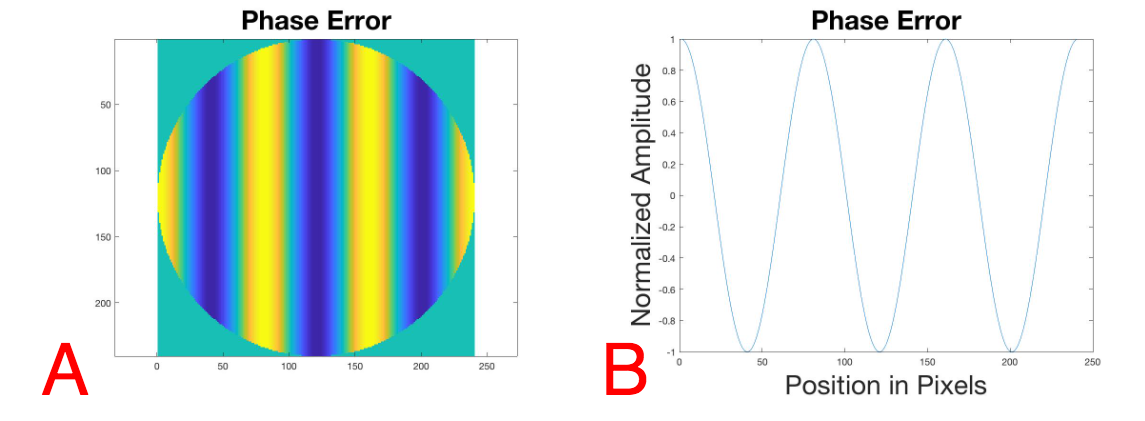
\includegraphics[width=0.8\textwidth]{Chapter Materials/Chapter Two Materials/CosinePhaseDiagram.png}
    \caption{A. Applied cosine phase error in radians in pupil plane to be propagated through the PWFS. B. Scaled cross section of the phase error.}
    \label{fig:CosinePhaseDiagram}
\end{figure}

\begin{figure}
    \centering
    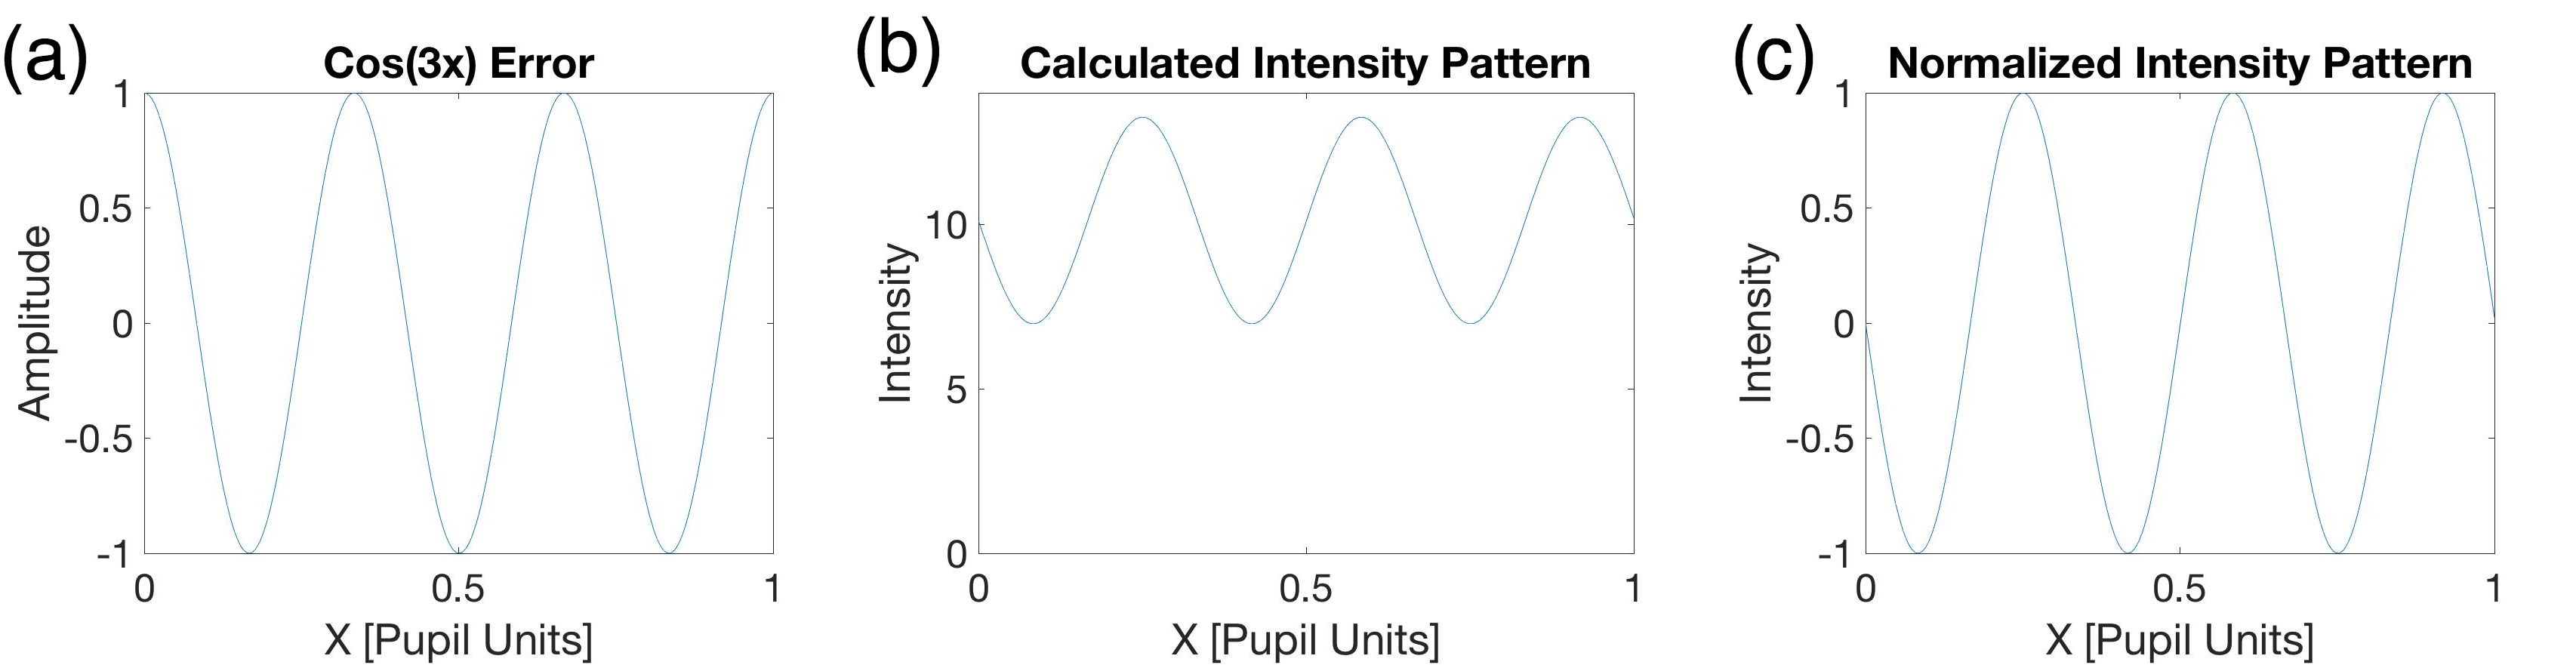
\includegraphics[width=1\textwidth]{Chapter Materials/Chapter Two Materials/MathPredictions.png}
    \caption{Predictions from the Foucault derivation. A. The applied $\cos(3x)$ phase error. B. The intensity pattern predicted for a single pupil. C. The expected pyramid signal after subtracting off constant terms and scaling.}
    \label{fig:MathPredicions}
\end{figure}

The resulting intensity patterns from the 3PWFS and 4PWFS are shown in Figure \ref{fig:IntensityPatternsDiagram} A and B. In Figure \ref{fig:IntensityPatternsDiagram} C and D we take a cross section from one of the pupils from each wavefront sensor and scale the signal. We then plot this against the predicted scaled intensity pattern. We find that the mathematical prediction is a good match for the measured intensity pattern inside the pupil of a modulated pyramid when the signal is linear. 


\begin{figure}
    \centering
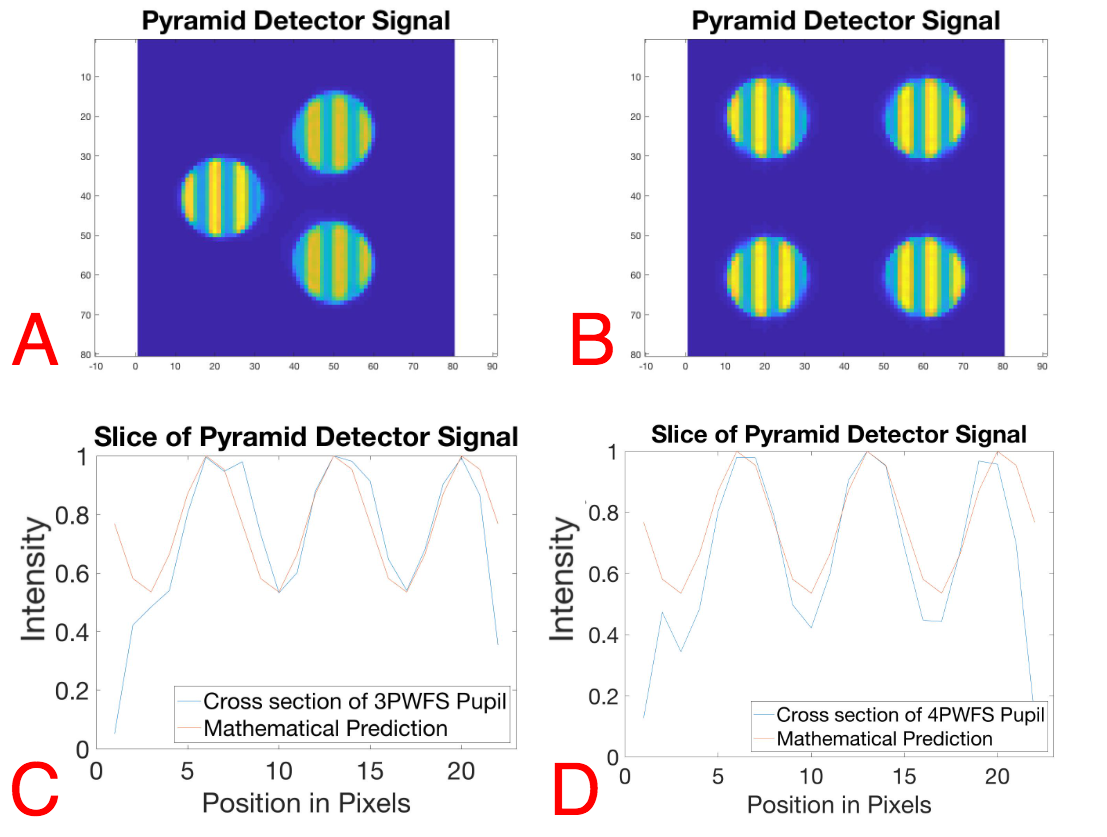
\includegraphics[width=0.8\textwidth]{Chapter Materials/Chapter Two Materials/IntensityPatternsDiagram.png}
    \caption{Resulting intensity patterns on the PWFS detector from A. the 3PWFS, and B. the 4PWFS. Figures C. and D. are cross section of the intensity pattern plotted against the mathematical prediction. For C. The cross section was taken from center of the middle-left pupil. For D. The cross section was taken from the center of the top two pupils.}
    \label{fig:IntensityPatternsDiagram}
\end{figure}

To gain further clarity we use the Slopes Maps equation that subtracts off the constant intensity and turns the signal into a pure X and Y measurement of phase. The Slopes Maps naturally subtracts the flat wavefront response and in that way is self-referencing.  More details on the Slopes calculation  for the 3PWFS is in Section~\ref{Slopes}. The Slopes Maps for the 3PWFS and the 4PWFS are shown in Figure \ref{fig:SlopesMapDiagram}, as well as the cross sections that are indeed a $-\sin(nx)$ function. 

\begin{figure}
    \centering
    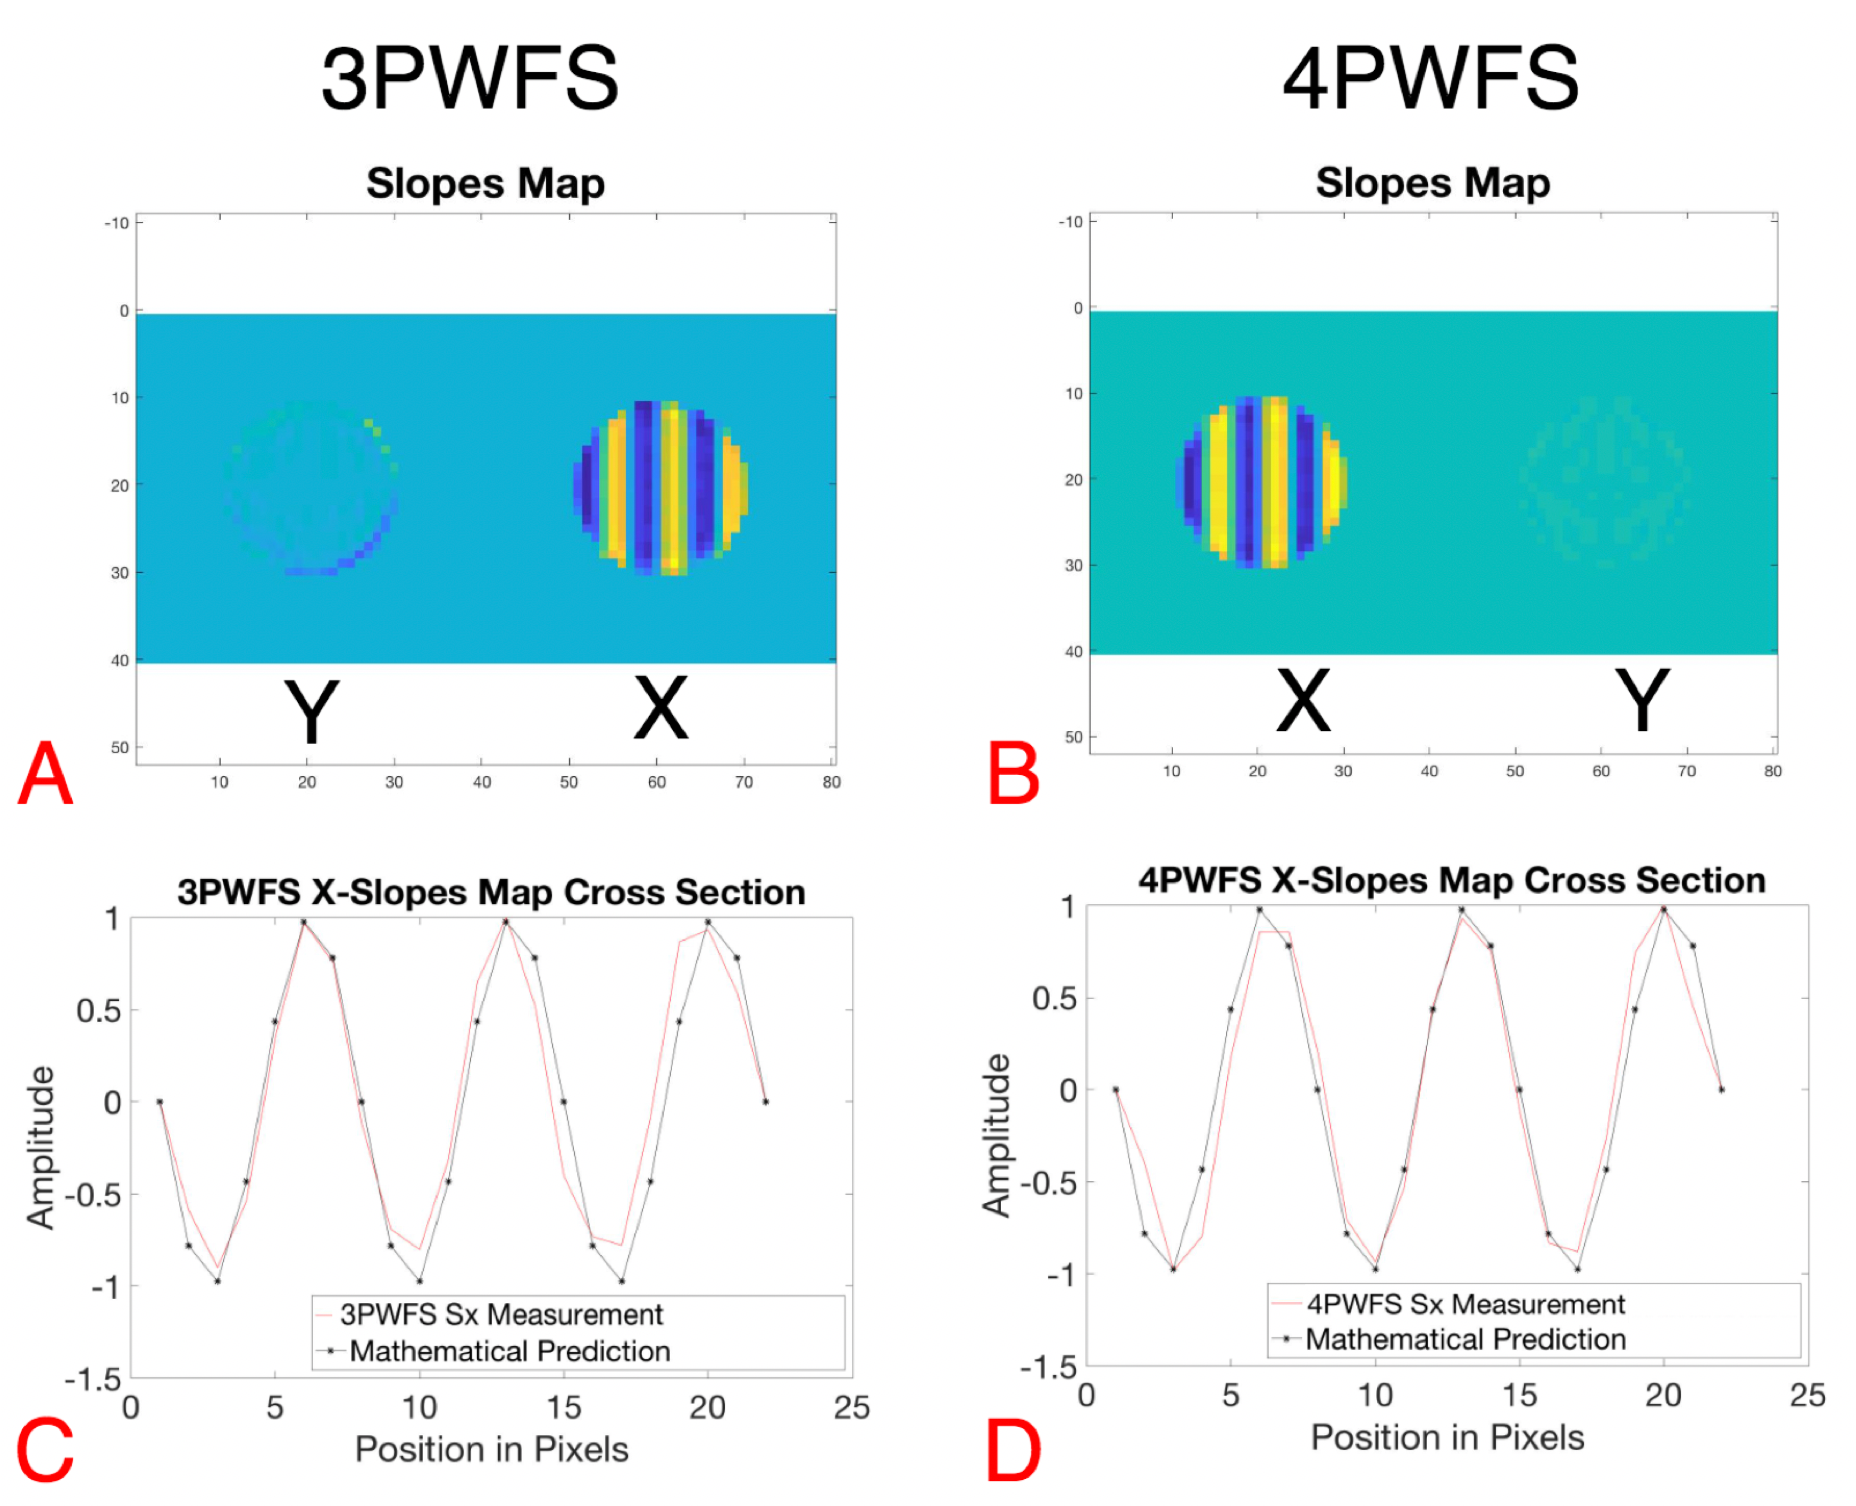
\includegraphics[width=0.9\textwidth]{Chapter Materials/Chapter Two Materials/SlopesMapsAndSlices.png}
    \caption{A. and B. Calculated slopes from the pyramid pupils. C. and D. Cross section of the Slopes plotted against the predicted signal. }
    \label{fig:SlopesMapDiagram}
\end{figure}

The previous simulations were performed with $5\lambda/D$ modulation. We can consider the 0 modulation case, which is a more direct relation to the results from the derivation. The unmodulated PWFS signal is more nonlinear than the modulated pyramid and therefore the fit between the prediction and the measured signal will be poor. In the case of the Slopes Maps signal, we found in simulation that the self-referencing is degraded from a nonlinear signal, and to return to a closer estimate of the signal the flat wavefront reference signal should be subtracted off. The fit worsens for the Slopes Maps without reference subtraction when there is a misregistration of the pupils, as will always be the case for the 3PWFS. For the 3PWFS subtracting off a reference improved the mean square error of the fit of simulation to derivation by about a factor of two, from 0.216 without subtraction, to 0.098 in the reference subtracted case. Figure \ref{fig:Mod0} summarizes the findings from the simulations with 0 modulation. Figure \ref{fig:Mod0}.A and \ref{fig:Mod0}.B are the detector signal of the 4PWFS and 3PWFS to the $\cos(3x)$ phase error. Figure \ref{fig:Mod0}.C and \ref{fig:Mod0}.D are a cross section of the scaled Slopes Maps plotted against the predicted signal. Figure \ref{fig:Mod0}.E and Figure \ref{fig:Mod0}. F are cross sections of the Slopes Maps with the reference signal subtracted.

\begin{figure}
    \centering
    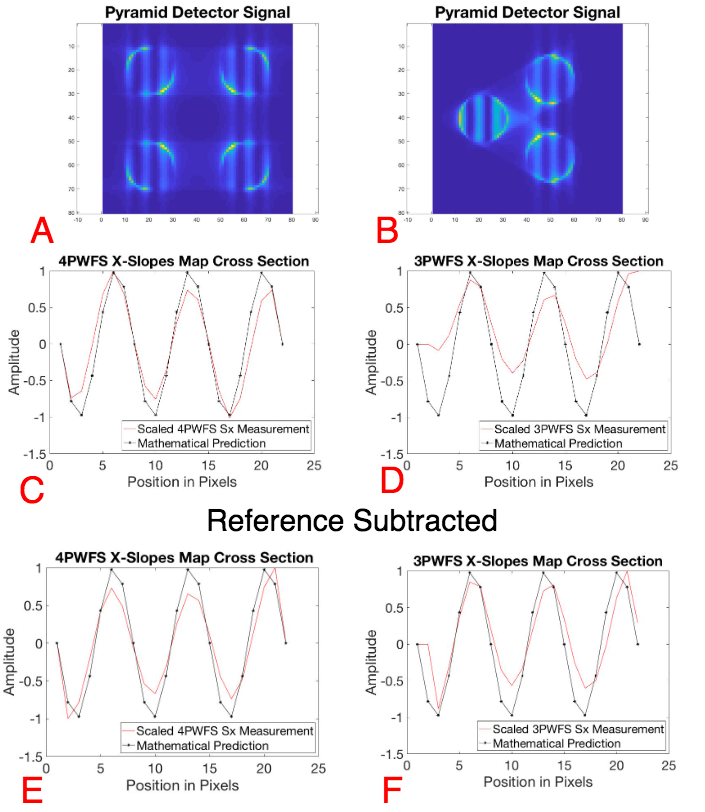
\includegraphics[width=0.9\textwidth]{Chapter Materials/Chapter Two Materials/Mod0PredictionVsSIm.png}
    \caption{A. and B. The wavefront sensor detector signals. C. and D. cross section of the wavefront sensor Slopes Maps plotted against the prediction. E. and F. the cross section of the Slopes Maps with the reference signal subtracted.}
    \label{fig:Mod0}
\end{figure}

The diffraction theory of the Foucault test predicts an intensity pattern that is the Hilbert transform of the wavefront phase. The result is an intensity pattern that is related to the wavefront derivative, but is not quite the derivative. In the case of a derivative wavefront sensor such as the Shack-Hartmann, the operation of the wavefront sensor on the phase to signal measurement is $\frac{d}{dx}\cos(nx)=-n\sin(nx)$. In the case of the pyramid the reference subtracted result is  $\frac{d}{dx}\cos(nx)=-\sin(nx)$, which is similar to the derivative wavefront sensor but without the scaling by spatial frequency. The result is that the knife edge and therefore the unmodulated pyramid sensitivity does not depend on spatial frequency, because all spatial frequencies will produce an equally strong signal. In the Shack-Hartmann case the strength of the signal scales linearly with spatial frequency.


\section{3PWFS Slopes Maps}\label{Slopes}

\subsection{Derivation}\label{SlopesDerivation}

The Slopes Maps technique was derived for the 4PWFS using the same intensity centroid calculation as a Shack-Hartmann wavefront sensor. The Shack-Hartmann uses a quad-cell intensity calculation to track the movement of spots to calculate the X and Y gradient of the wavefront phase in post-processing. In the geometric optics approximation the PWFS acts as a slope sensor, and the Slopes Maps calculates the wavefront gradients in a similar way to the Shack-Hartmann. In the diffractive optics derivation, the wavefront slopes are calculated by the diffraction of the pyramid edges and encoded directly into the intensity pattern. We do not need to perform a Slopes Maps calculation for the pyramid signal because we are directly measuring a function that is related to the gradient phase error, but it is still beneficial to do so. The Slopes Maps is the natural recombination of the pyramid signals that subtracts off the constant Intensity pattern, so a reference image is not required. In a closed loop system the wavefront signal is driven towards  zero slope which arises when the PSF is centered on the pyramid tip with no phase errors. The Slopes Maps technique suffers from misalignments of the pyramid pupils; any misregistration in the sampling of the pupils with respect to each other results in a loss of performance. 

The Slopes Maps for the 4PWFS is already known. In previous work by Costa \cite{buchler2004development}, a Slopes Map calculation for the 3PWFS was derived assuming a geometric optics approximation of the PWFS as a derivative wavefront sensor in the modulation regime. In this paper we introduce a new Slope Maps method to handling the 3PWFS signals, which is derived using the intensity centroid of an equilateral triangle.

To calculate the Slopes Maps equations for the 3PWFS, we start from the same assumptions used for the 4PWFS. We assume that the maximum sensitivity of the sensor occurs when the PSF is centered at the tip of the four pyramid edges. We seek a Slopes Maps equation that drives the wavefront to zero slope, resulting in uniform intensity in the re-imaged pupils. To derive the centroid equation for the 3PWFS we start with an equilateral triangle, shown in Figure \ref{fig:triCentFig}. The center of the triangle is at the origin of a Cartesian coordinate system, and the vertices of the triangle are all an equal distance from the origin. The blue circles represent the layout of the pupils on the PWFS detector, and $I_1$ corresponds to $(x_1, y_1)$, etc. Solving for the coordinates $(x_1,y_1),(x_2,y_2), (x_3,y_3)$ gives the weights in the $S_x$ and $S_y$ Slopes Maps. 

% We can see in Equation~\ref{4PWFSslopes} that when the pixel values are equal the value of the Slopes are zero.

\begin{figure}
\begin{center}
\begin{tabular}{c}
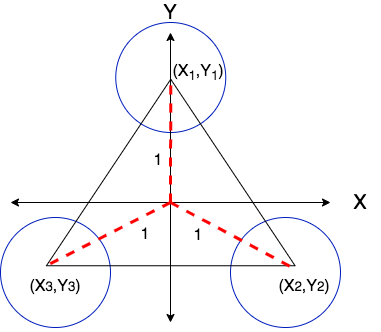
\includegraphics[height=5.5cm]{Chapter Materials/Chapter Two Materials/3PWFSslopesMap.png}
\end{tabular}
\end{center}
\caption 
{ \label{fig:triCentFig}
Equilateral triangle with the center at the origin. Solving for the coordinates of the vertex points gives the weights for the pixel Intensities used in the Slopes Maps calculation. The blue circles represent the layout of the pupils on the detector. } 
\end{figure} 

For the 3PWFS we find that the $S_x$ and $S_y$ Slopes Maps are,
% \begin{equation}
%     S_x=\frac{\frac{\sqrt{3}}{2}I_2-\frac{\sqrt{3}}{2}I_3}{I_1+I_2+I_3}, \; \;
%     S_y=\frac{I_1-\frac{1}{2}I_2-\frac{1}{2}I_3}{I_1+I_2+I_3}
%     \label{3PWFSslopes}
% \end{equation}

\begin{eqnarray}
    S_x=\frac{\frac{\sqrt{3}}{2}I_2-\frac{\sqrt{3}}{2}I_3}{I_1+I_2+I_3} \label{3PWFSslopes} \\
    S_y=\frac{I_1-\frac{1}{2}I_2-\frac{1}{2}I_3}{I_1+I_2+I_3} \nonumber
\end{eqnarray}

The $S_x$ slopes maps in this orientation depends only on the intensities from the $I_2$ and $I_3$ pupil pixels which act as a roof sensor. The result is that care must be taken to properly index the pupils when applying the Slopes Map equation. 
 
 \subsection{Testbed Verification}
 
To test the validity of the Slopes Maps equation for the 3PWFS, and the Raw Intensity method we implemented these signal processing methods into a real closed adaptive optics system using the LOOPS testbed at the Laboratoire d'Astrophysique de Marseille. The LOOPS testbed at LAM used a spatial light modulator (SLM) to create the pyramid tip. A full description of the LOOPS testbed can be found in Janin-Poitron et. al. 2019 \cite{janin2019adaptive}. On the testbed a closed loop correction was achieved for both a 3PWFS and 4PWFS with reconstructors calculated from both the Raw Intensity and Slopes Maps signal handling techniques. A reflective phase plate was used in the system to simulate turbulence, and an ALPAO deformable mirror was used to apply the correction. In all cases a stable closed loop was obtained. Figure \ref{fig:LOOOPS} shows example images from the LOOPS test-bed of (A) the pyramid signal of the 3PWFS under turbulence in closed loop, (B) the pyramid signal of the 4PWFS under turbulence in closed loop, (C) the LOOPS PSF with no turbulence, and (D) the LOOPS PSF in closed loop with the 3PWFS using the Slopes Map technique. 

\begin{figure}
    \centering
    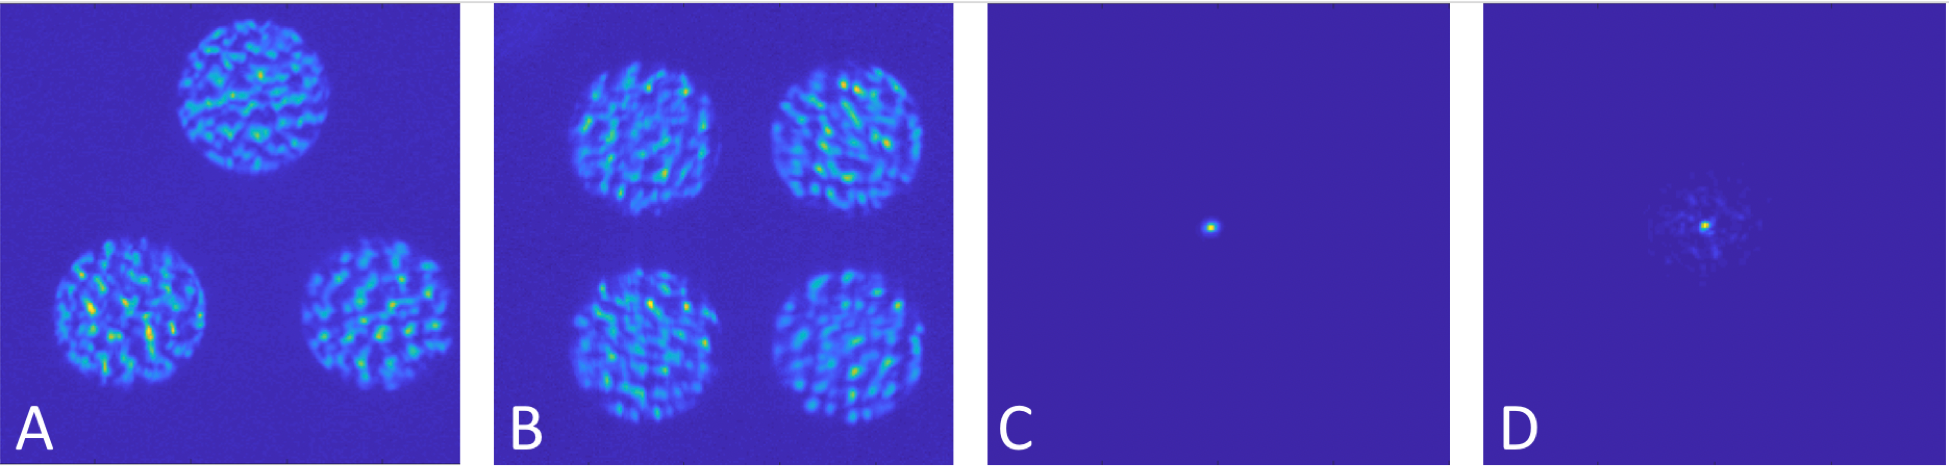
\includegraphics[width=0.8\textwidth]{Chapter Materials/Chapter Two Materials/LOOPS.png}
    \caption{Example images from the LOOPS test-bed of A) the pyramid signal of the 3PWFS under turbulence in closed loop, B) the pyramid signal of the 4PWFS under turbulence in closed loop, C) the LOOPS PSF with no turbulence, and D) the LOOPS PSF in closed loop with the 3PWFS using the Slopes Map technique.}
    \label{fig:LOOOPS}
\end{figure}

\section{The Reconstructor Matrix}

In the previous sections we have derived what the expected signal is from the pyramid wavefront sensor, and how to process the signal to retain only the intensity pattern due to phase errors. Now we will explore how we take the processed wavefront sensor signals and build a reconstructor matrix that allows us to reconstruct the wavefront error. 
 
The wavefront sensor measures a signal $S$, which includes the signal processing discussed in Section \ref{PWFSintro}. The signal can be decomposed into a summation of modes from a basis set. The interaction matrix $I$, is the bridge between the deformable mirror commands and the wavefront signals. The interaction matrix is calibrated by applying modes on the deformable mirror and recording the response from the wavefront sensor. The intensity measurements are unraveled from a 2D detector image into a 1D vector and stored as a column vector in the interaction matrix. We can use the interaction matrix to apply shapes on the deformable mirror by summing modes that are weighted by amplitudes stored in the amplitude matrix $A$. The interaction matrix and the amplitude matrix are related to an wavefront sensor signal by $S=IA$. In the AO case, we measure $S$, which is a $[M\times 1]$ matrix of wavefront sensor signals from aberrated starlight, and calibrate to find $I$ which is a $[M\times N]$ matrix. To reconstruct the signal we need to find $A$, a $[N\times 1]$ matrix the corresponding amplitudes that will give us the right wavefront shape. We cannot compute the operation $A=I^{-1}S$, because $I$ is an $[M\times N]$ size matrix and not invertible. To find $A$, a pseudo-inverse of $I$ is calculated using singular value decomposition (SVD). The SVD of I is calculated by,

\begin{equation}
    SVD(I)=U\Sigma V^T
\end{equation}

where $U$ is a $[M\times M]$ matrix, $Sigma$ is an $[M\times N]$ matrix with singular values on the diagonal, and $V$ is an $[N\times N]$ matrix. We calculate the reconstructor matrix $R$ which is the pseudo-inverse of $I$ using $U$,$V$,and $\Sigma$.

\begin{equation}
   R=V\Sigma^{\dag}U^T
\end{equation}

The Reconstructor matrix R is a $[N\times M]$ sized matrix, and we calculate the vector of modal amplitudes using equation \ref{ReconEq}.

\begin{equation}
    A=RS
    \label{ReconEq}
\end{equation}

An additional matrix $C$ of size $[K\times N]$ that is the commands to drive the deformable mirror to shapes that are modes in the basis set is needed. The amplitude matrix $A$ scales this command matrix so that the proper amplitude of each mode is applied. The multiplication $CA$, gives a $[K\times 1]$ vector that are the deformable mirror commands. Reshaping the $[K\times 1]$ matrix into a $[\sqrt{K}\times \sqrt{K}]$ matrix gives the command for each actuator in the deformable mirror, where the deformable mirror is a square of $\sqrt{K}\times \sqrt{K}$ actuators.
\chapter{Design of the MagAO-X wavefront sensor}

\section{Introduction to Optical Design}

The basis of optical design is to design a system that meets given requirements and minimizes optical aberrations in the system. Optical designers use geometric optics to calculate the size and location of first order parameters in the optical system, which include the pupil planes, focal planes, stops, and nodal points. In geometric optics light is treated as a ray that is traced point to point through the optical system. The result is that one point in the image plane maps to one point in the object plane. It can model the effects of optical aberrations to calculate the error in ray propagation called optical path difference (OPD) for different ray heights and angles. Geometric optics cannot be used to predict the effects of the wave nature of light, such as diffraction and interferometry. 

Paraxial optics is a simplification to geometric optics that assumes the small angle approximation. It is a method for solving for the first order properties of a system using ray tracing equations. The paraxial approximation ignores the curvature of surfaces, but does take into account refraction through materials. The paraxial raytrace equations are,

\begin{eqnarray}
       n'u'=nu -y\phi  \label{4PWFSslopes} \\
       y'=y+u't' \nonumber \\
       \phi =(n'-n)C
\end{eqnarray}

where $n$ and $n'$ are the refractive index of the medium before and after propagation. The variables $u$ and $u'$, are the ray angles and $y$ and $y'$ are the ray heights. The distance between the starting point and the propagated point is $t'$. The variable $\phi$ is the power of a surface with curvature $C$ and refractive index $n'$. Figure \ref{fig:paraxial} shows an example setup of a raytrace,(\cite{greivenkamp2004field}). Various raytracing programs such as Zemax, CodeV, and Oslo implement paraxial raytracing modes to design optical systems. 


\begin{figure}
    \centering
    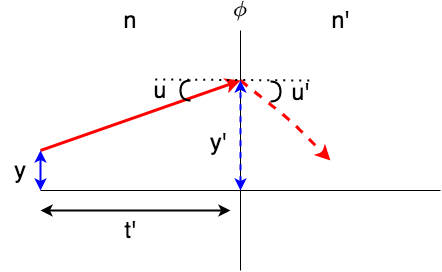
\includegraphics[width=.5\textwidth]{Chapter Materials/Chapter Three Materials/paraxialray.png}
    \caption{Setup for a paraxial ray trace. Starting point is from an object height $y$, with angle $u$. The ray is propagated a distance $t'$, until it hits a surface with power $\phi$, and refractive index $n'$. The ray height at this surface is $y'$, and exits with angle $u'$.}
    \label{fig:paraxial}
\end{figure}




Tracing the marginal and chief ray using the paraxial raytracing method determines important system parameters. The marginal ray has zero height at the object, passes through the maximum edge of the aperture stop, and is zero at the image plane. Tracing the marginal ray gives the positions of the object and image planes, and the height of the system stops. This includes the aperture stop, as well as the entrance and exit pupils of the system, which are the image of the aperture stop in the object and image planes respectively. The chief ray passes through the maximum edge of the object and image, and passes through the center of the aperture stop. It gives the object and image sizes as well as the location of the system stops. Figure \ref{fig:chiefray} shows an example ray trace of the marginal and chief ray through a lens with the stop at the lens. 


\begin{figure}
    \centering
    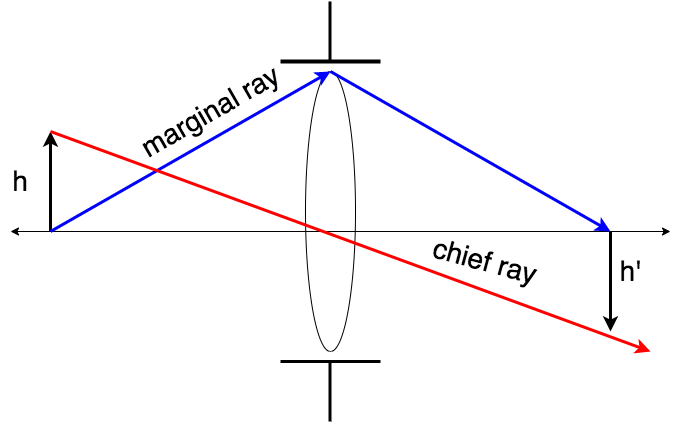
\includegraphics[width=.6\textwidth]{Chapter Materials/Chapter Three Materials/chiefandmarginal.png}
    \caption{Diagram of a ray trace for the marginal and cheif ray. The marginal ray starts at the optical axis at the location of the object, and is traced to the maximum edge of the system stop. It crosses the optical axis at the location of the image. The chief ray starts at the object height $h$, crosses the optical axis through the center of the stop, and intersects the maximum height of the image $h'$. }
    \label{fig:chiefray}
\end{figure}



Once the first order properties of the system are determined, the next step in the design process is to mitigate the optical aberrations that can be corrected for through design. A way to determine the aberrations in the system is to first trace the paraxial ray, and then trace a bundle of rays at different heights and angles of field to determine the deviation from the paraxial solution, which is the OPD. We describe these aberrations as coefficients in a power series. The wave aberration equations are useful because they allow us to calculate the wavefront error as a function of field, $H$, aperture vector, $\rho$, and the wavefront error coefficient for the associated aberration, $W_{ijk}$. The coordinate system for determining the wave aberrations is given in Figure \ref{fig:Seidel}. The generating function for the wave aberration polynomials is,


\begin{equation}
    W(H,\rho, \theta)=\sum_{ijk} W_{ijk} H^i \rho^j \cos^k\theta
\end{equation}

where $W(H,\rho, \theta)$ is the total wavefront error. We can use these polynomials to solve for ray aberrations $\epsilon$ which are the deviations from the paraxial image plane for the system in both the longitudinal (parallel to the optical axis), and transverse (perpendicular to the optical axis) directions. 

\begin{figure}
    \centering
    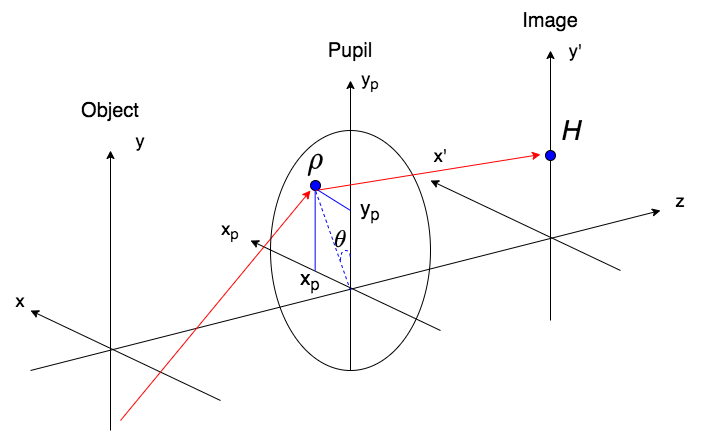
\includegraphics[width=.8\textwidth]{Chapter Materials/Chapter Three Materials/Seidelcoord.png}
    \caption{Coordinate system for the wave aberration polynomials. The field coordinate is given by $H$, and the location in the pupil plane is given by $\rho$. (FIGURE OUT HOW TO CITE CLASS NOTES THIS CAME FROM 503)}
    \label{fig:Seidel}
    \end{figure}
    
The first few aberrations can be mitigated by the optical design. The aberrations that are considered when designing a system are: defocus, tip/tilt, coma, astigmatism, spherical, field curvature, distortion, and chromatic aberration. These aberrations are first and third order abberations and the corresponding wave aberration equations that describe each aberration is found in Table \ref{tab:aberrations}. There are higher order variants of these polynomials, for example fifth-order astigmatism, but in general these terms are harder to correct and are compensated with first and third-order terms. Optical design programs have tools to help the designer reduce and balance the aberrations. Zemax OpticStudio outputs ray fan diagrams that describe the total OPD amplitude and shape as a function of $\rho$. Individual Seidel coefficients for specific aberrations can be minimized through the system optimization Merit function. Different weights in the merit function can prioritize the correction of one aberration over others. 


\begin{table}
	\begin{center}
		\begin{tabular}{ | l| l | }
			\hline
			\textbf{Aberration}& \textbf{Wave Aberration Equation} \\ \hline
			Defocus & $W_{020}\rho^2$\\ \hline
			Tip/Tilt & $W_{111}H\rho \cos\theta$ \\ \hline
			Coma & $W_{131}H\rho^3\cos\theta$  \\ \hline
			Astigmatism & $W_{222}H^2\rho^2\cos^2\theta$  \\ \hline
			Spherical Aberration & $W_{040}\rho^4$ \\ \hline
			Field Curvature & $W_{220}H^2\rho^2$ \\ \hline
			Distortion & $W_{311}H^3 \rho \cos\theta$ \\ \hline
				
		\end{tabular}
	\end{center}
	\caption{Caption}
	\label{tab:aberrations}
\end{table}

In free space optical design it is common to work with spherical lenses because they are easy to manufacture. These lenses can introduce significant spherical and chromatic aberrations into the optical system. In this section we will briefly describe these aberrations, and how to mitigate them through design.  

\subsection{Spherical Aberration}

Spherical aberration is defined as the variation of focus by position of the aperture. It is caused by spherical surfaces, and in lenses it is due to the variation of thickness of the glass as a function of aperture due to the curvature of the lens surfaces. For a converging lens the effect is that rays that intersect near the edges of the lens aperture are bent more, and come to a focus before the rays that pass closer to the center. This effect is shown in Figure \ref{fig:spherical}. 

\begin{figure}
    \centering
    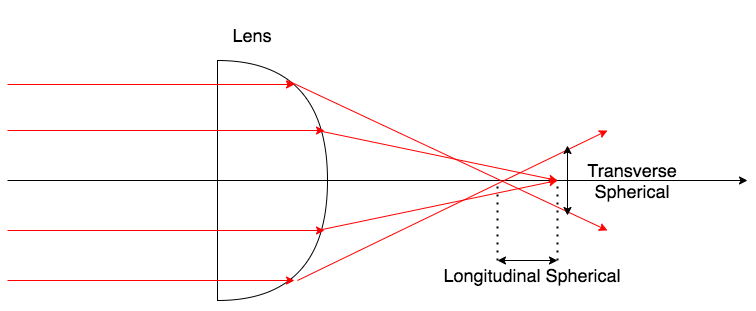
\includegraphics[width=.8\textwidth]{Chapter Materials/Chapter Three Materials/spherical.png}
    \caption{Diagram of rays incident on a plano-convex lens. The effect of spherical aberration can be seen by rays that are closer to the edges of the lens coming to a focus before those that are closer to the center of the lens. }
    \label{fig:spherical}
\end{figure}

There are a number of ways spherical aberration can be minimized in an optical system. The simplest method is to balance spherical aberration with defocus. This method is not ideal because there can be significant residual wavefront error. For custom lens design splitting the lens into a doublet ] to lessen the curvature of the surfaces reduces third spherical aberration by about a third or a fourth. Changing the shape factor of the lens changes the curvature and thickness of the lens while maintaining focal length. The shape factor is a measure of overall curvature of a lens and is calculated using,

\begin{equation}
    X=\frac{C_1-C_2}{C_1+C_2}
\end{equation}
where $C_1$ and $C_2$ are the front and back curvatures of the lens. Lenses with high shape factors have extreme curvatures and large spherical aberrations. Figure \ref{fig:shapefactor} compares lenses with the same focal lengths with high shape factor (A), and low shape factor (B). Making a surface of the lens aspheric or introducing an aspheric corrector plate can be used to illuminate or correct spherical aberration. Aspheric surfaces are harder to manufacture and increase system cost and complexity. Aberrations scale with the index of refraction. Using a lens made of a glass with high refractive index reduces spherical aberrations. There are other tricks for reducing spherical aberrations such as exploiting stop locations, that are more system specific and might not be applicable to all optical designs. 

\begin{figure}
    \centering
    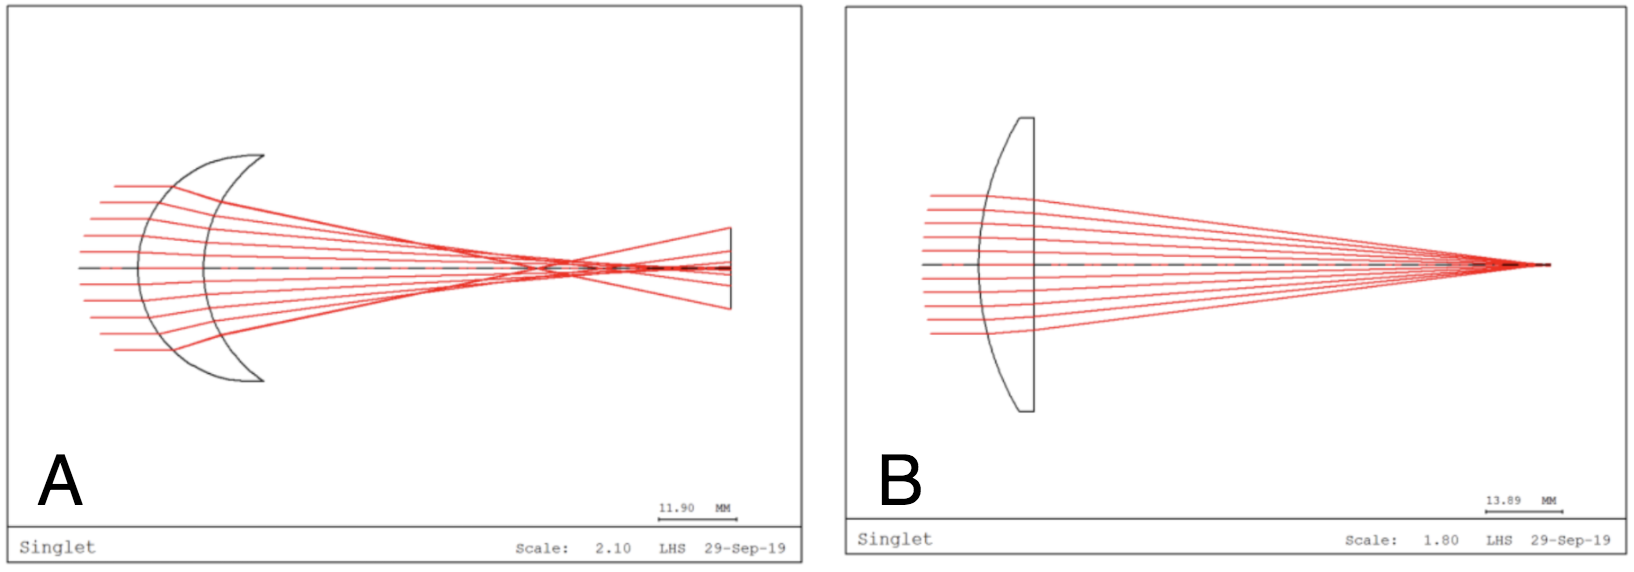
\includegraphics[width=.8\textwidth]{Chapter Materials/Chapter Three Materials/ShapeFactor.png}
    \caption{ Diagram of the effect of shape factor on the amount of spherical aberration of lens made in Zemax. A. This lens has a shape factor 5 and exhibits strong spherical aberration due to the extreme curvature of the lens surfaces. B. Lens with a shape factor 1. Spherical aberration is minimized.}
    \label{fig:shapefactor}
\end{figure}


\subsection{Chromatic Aberrations}

Chromatic aberration is caused by the wavelength dependence of the index of refraction, which causes the refracted angle of a light ray to change according to wavelength. The effect of longitudinal chromatic aberration is that different wavelengths come to a focus at different points on the optical axis. Lateral chromatic aberration causes a variation in image magnification as a function of wavelength. We measure the amount of chromatic aberration with respect to different Fraunhofer absorption lines; the F line at $\lambda_F=486.1 nm$, the D line at $\lambda_D=589.2 nm$, and the C line at $\lambda_C= 656.3 nm$. The chromatic focal shift, $\delta_{FC}$,  is given calculated with respect to the $F$ and $C$ lines and is given by,

\begin{equation}
    \delta_{FC}=\frac{\phi_F-\phi_C}{\phi_F \phi_C}
\end{equation}


where $\phi$ is the optical power of the lens at those wavelengths. In optical design we measure the chromatic focal shift as a function of wavelength. Figure \ref{fig:focalshift} shows the chromatic focal shift of a singlet lens made of BK-7 glass.

\begin{figure}
    \centering
    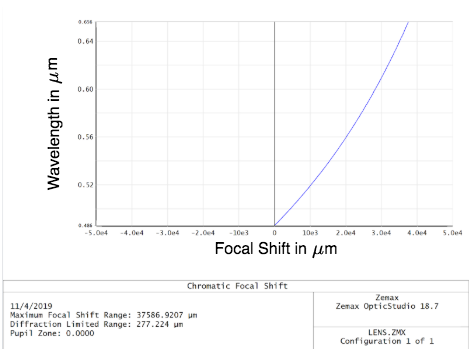
\includegraphics[width=.7\textwidth]{Chapter Materials/Chapter Three Materials/focalshift.png}
    \caption{Diagram of the chromatic focal shift of a singlet lens made of BK-7 glass. The shift in focal length due to chromatic aberration is plotted agains wavelength.}
    \label{fig:focalshift}
\end{figure}

To correct for chromatic aberration we try and balance the chromatic focal shift by constructing a lens that places two or more wavelengths at the same focal length. For a single lens system we compensate the chromatic error by constructing achromatic doublets and triplets. An achromatic doublet is a pair of lenses, usually one positive lens and one negative lens, made of different materials that form a single lens. These lenses can be air spaced or cemented together. The crown glass is usually used for the positive lens, and the flint glass for the negative lens. An example of a crown-flint achromatic doublet designed in Zemax is shown in Figure \ref{fig:crownflint}.

\begin{figure}
    \centering
    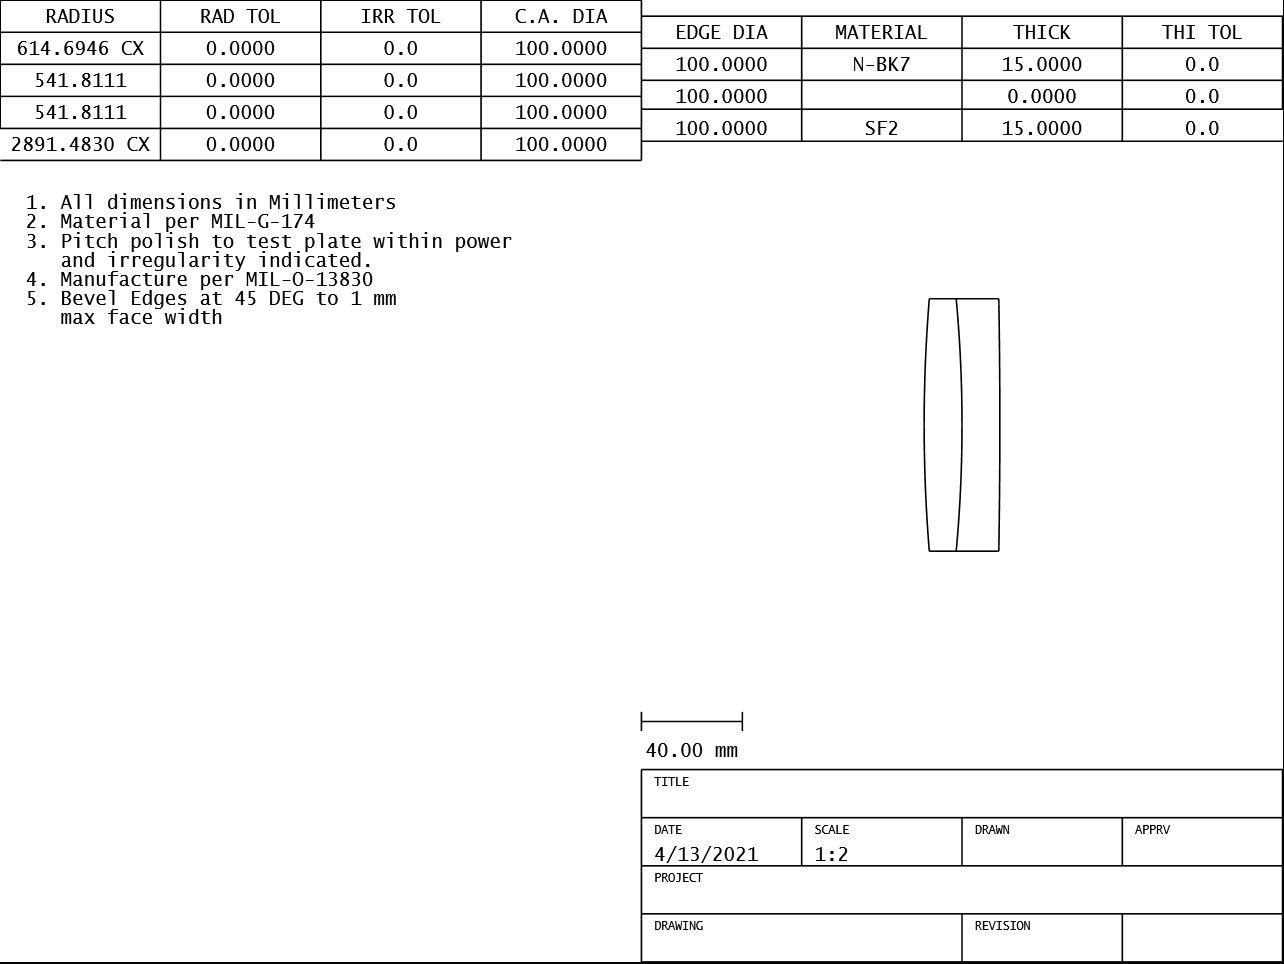
\includegraphics[width=.8\textwidth]{Chapter Materials/Chapter Three Materials/doublet.jpg}
    \caption{Diagram of an achromatic doublet. The first lens is a positive lens made of crown glass. The negative lens is made from flint glass. }
    \label{fig:crownflint}
\end{figure}

The Abbe number, $\nu_d$, of a glass quantifies the material's dispersion. It is calculated by the using the refractive index of the material ad the F,D, and C lines. The equation for Abbe number is given in Equation \ref{abbe}. 

\begin{equation}
    \nu_d=\frac{n_D-1}{n_F-n_C}
    \label{abbe}
\end{equation}

Low Abbe numbers correspond to high dispersion. One of the lenses in the doublet is made from a type of glass called a crown glass that has a low refractive index, and low dispersion. The other lens is made of a flint glass, which has a high refractive index and a high dispersion. The combination of the two glass types corrects for chromatic aberrations by shifting the F and C focal lengths close together. In general this is best achieved when there is a large difference in the Abbe numbers of the glasses. The system of equations used to solve for the power of each lens is,
%
\begin{eqnarray}
       \delta \phi_{FC}=\phi_F-\phi_C=0 \\
       \frac{\phi_{1}}{\phi_T}= \frac{\nu_1}{\nu_1-\nu_2} \\
       \frac{\phi_{2}}{\phi_T}= \frac{-\nu_2}{\nu_1-\nu_2}\nonumber
\end{eqnarray}
where $\phi_T$ is the total system power, and $\phi_1$ and $\phi_2$ are the the power of each lens at the D wavelength. Figure \ref{fig:doublet} shows an example chromatic focal shift diagram created by an achromatic doublet made from BK-7 and F4 glass. 

\begin{figure}
    \centering
    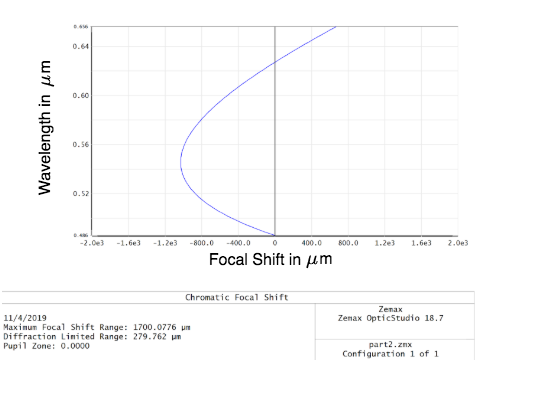
\includegraphics[width=.8\textwidth]{Chapter Materials/Chapter Three Materials/doubletfocalshift.png}
    \caption{Focal shift diagram of an achromatic doublet from BK-7 and F4 glass. Achromatic doublets balance chromatic aberration by setting the focal shift of two different wavelengths in the bandpass to 0.}
    \label{fig:doublet}
\end{figure}

Achromatic triplets correct for both chromatic aberration and secondary chromatic aberration. Secondary chromatic aberration, or secondary spectrum, is caused by the third D wavelength coming to focus at a different spot than the focal shift corrected F and C wavelengths. Minimizing the focal shift between all three wavelengths is the method of correcting for secondary spectrum. Secondary chromatic aberration is compensated by considering the dispersion $P$ of a material, given by Equation \ref{dispersion}. The secondary chromatic aberration is controlled by choosing glasses that have very similar dispersion, but a large difference in Abbe number. 

\begin{equation}
    P=\frac{n_d-n_c}{n_F-n_C}
    \label{dispersion}
\end{equation}



A apochromatic lens is a triplet lens that balances the chromatic focal shifts and secondary chromatic aberrations at three wavelengths. The system of equations for the apochromatic triplet is,


\begin{eqnarray}
       \phi_1=\frac{(P_2-P_3)\nu_1}{(P_2-P_1)E}\phi_T \\
       \phi_2=\frac{(P_3-P_1)\nu_2}{(P_2-P_1)E}\phi_T \\
       \phi_3=\frac{(P_1-P_2)\nu_3}{(P_2-P_1)E}\phi_T \\
       E=\frac{(P_2-P_3)\nu_1+(P_3-P_1)\nu_2}{(P_2-P_1)}-\nu_3
\end{eqnarray}
where $P_1$,$P_2$, and $P_3$ are the dispersion's of each of the lenses in the triplet. The solution to these equations is that glass 1 and 3 should have very different dispersions and Abbe numbers to minimize chromatic aberrations, and that the second glass should have a $P$ and $\nu$ value that falls in between roughly halfway between the two. This is best visualized in Figure \ref{fig:tripletPV}, which plots the dispersion vs Abbe number for the different glass types in a triplet. 
\begin{figure}
    \centering
    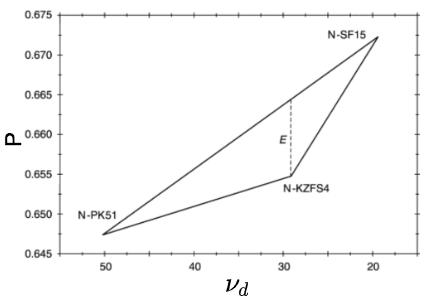
\includegraphics[width=.6\textwidth]{Chapter Materials/Chapter Three Materials/tripletPV.png}
    \caption{Dispersion $P$ versus Abbe number $\nu_d$ for an achromatic triplet made from N-PK51, N-KZFS4, and N-SF15 glass types, (\cite{kingslake2009lens}).} 
    \label{fig:tripletPV}
\end{figure}

The resulting chromatic focal shift diagram for a triplet lens has three zero points as shown in Figure \ref{fig:apochromat} for a 100mm focal length apochromatic triplet made of N-LLF1,N-LAF33, and N-BK7 glass types by \cite{sasian2017method}. 

\begin{figure}
    \centering
    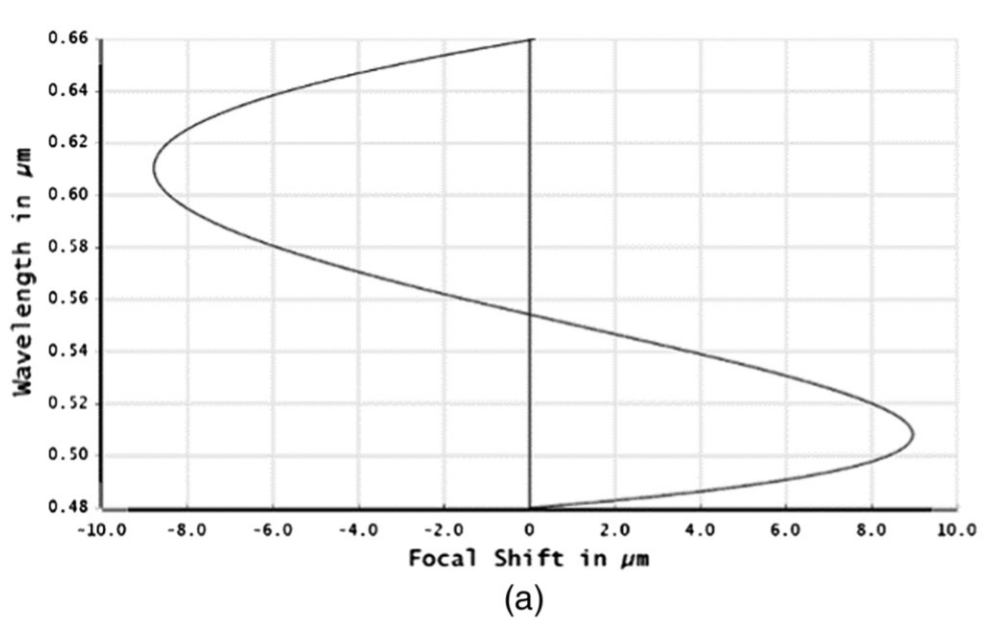
\includegraphics[width=.6\textwidth]{Chapter Materials/Chapter Three Materials/tripleapochromat.PNG}
    \caption{Chromatic focal shift diagram for an apochromatic triplet lens. The first and secondary chromatic aberrations are compensated in the lens creating three wavelengths where a zero chromatic focal shift occurs,(\cite{sasian2017method}).}
    \label{fig:apochromat}
\end{figure}









\section{MagAO-X}
	
the University of Arizona Extreme Wavefront Control Lab (XWCL), has developed the Magellan Extreme Adaptive Optics system (MagAO-X) for the Magellan Clay Telescope at Las Campanas Observatory, Chile,(\cite{males2020magao}). MagAO-X had its first light commissioning run in 2019b. The MagAO-X system uses a combination of a 2048 actuator deformable mirror, high speed pyramid wavefront sensor, and high contrast coronagraph to correct for atmospheric turbulence and suppress starlight at speeds greater than 2000 times a second. The instrument is designed to achieve Strehl ratios of greater than 70$\%$ with raw contrast of less than $10^{-4}$ at separations between 1 and 10 $\lambda/D$.\cite{males2018magao} Working off of lessons learned from MagAO ,(\cite{close2018status}), and SCExAO, (\cite{jovanovic2015subaru}), MagAO-X is optimized for high impact science cases, such as a survey of nearby newly formed acretting planets in H$\alpha$, (\cite{males2020magao}).

The MagAO-X system has a two-level split optical table, mounted at the gravity invariant Nasymth platform. The table is floated to reduce vibrations, and sealed in dust covers to shield against dust and stray light. The top optical table contains the K-mirror, (\cite{hedglen2018optical}), the low order ALPAO DM97 woofer deformable mirror, the high order tweeter BMC-2K deformable mirror, and the atmospheric dispersion corrector (ADC). The lower bench contains another ALPAO DM97 DM to correct non common path errors in the coronagraphs. There are two Princeton science camera to enable spectral differential imaging, (\cite{biller_sdi}). MagAO-X has a generalized Lyot coronagraph with a vector Apodizing Phase Plate (vAPP) mask. A four-sided pyramid PWFS provides the high order wavefront sensing. Figure REF shows the layout of the MagAO-X system. In this chapter we will describe the optical design of the MagAO-X pyramid wavefront sensor and the requirements on performance that drove the design choices. 

MAGAO-X FIGURE CHECK THE BOX

\section{System Design}

The PWFS of the MagAO-X system consists of an achromatic pyramid, a camera lens, and an OCAM$^2$K EMCCD detector. The requirements on the MagAO-X PWFS were a needed size and separation of the pupils, and a restricted system size to fit on the optical table. The MagAO-X pyramid wavefront sensor is designed to operate from 600-1000nm bandwidth and a field of view of two arcseconds. Figure \ref{fig:bandpass} is the bandpass of the MagAO PWFS that we matched for the MagAO-X PWFS. A new camera lens was designed in Zemax to meet the requirements of the MagAO-X system. 
	
	
\begin{figure}[h]
	\centering
	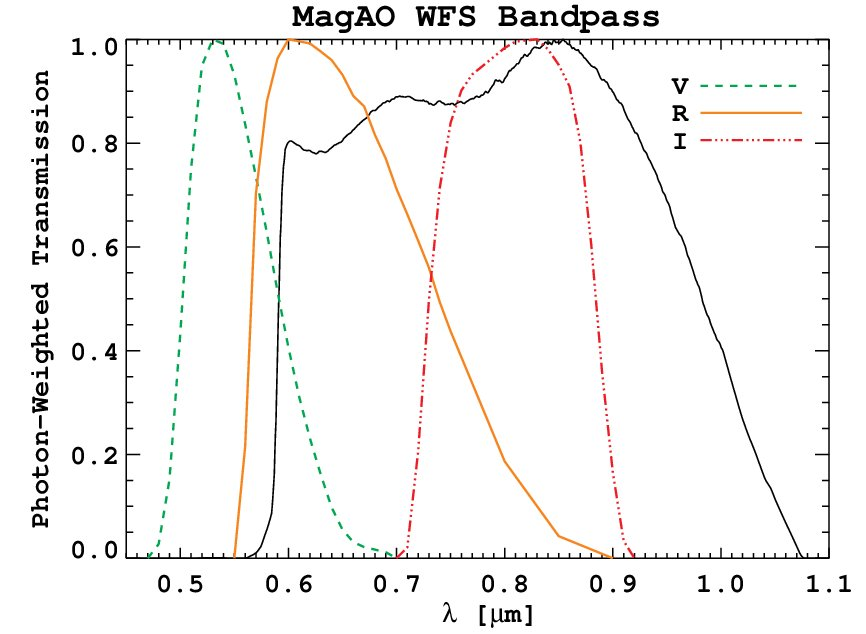
\includegraphics[width=.5\textwidth]{Chapter Materials/Chapter Three Materials/MagAOBandpass_updated.jpg}
	\caption{Transmission versus wavelength for the V, R, and I bandpasses. The overlaid black curve is MagAO-X pyramid wavefront sensor bandpass that is matched from MagAO,(\cite{morzinski2014magao}).}
	\label{fig:bandpass}
\end{figure}
	
 The requirements of the MagAO-X PWFS are listed in Table \ref{tab:requirements}. The OCAM$^2$K is used in the 2x2 binning mode, which gives and effective pixel size of 48 $\mu$m. This allows the wavefront sensor to be run at speeds up to 3.6 kHz. The pupil size is 56 pixels in diameter. The number of pixels in each of the pupils sets the sampling of the wavefront which determines the number of modes correctable by the AO system and the fitting error in the AO error budget. This sampling was chosen to meet the performance goals of the MagAO-X wavefront control. The pupil separation of 60 pixels was chosen to maximize space on the OCAM$^2$K detector. Figure \ref{fig:PWFSpupils} summarizes the desired layout for the PWFS pupils on the OCAM$^2$K detector. 
	
\begin{table}
	\begin{center}
		\begin{tabular}{ | l| l | }
			\hline
			\textbf{Parameter}& \textbf{Requirement} \\ \hline
			Wavelength Range &600- 1000 nm \\ \hline
			Pupil Size & 56 pixels; 2.688 mm \\ \hline
			Pupil Separation & 60 pixels; 2.880 mm  \\ \hline
			Pupil Tolerances & $\Delta$ $<$ 1/10th pixel; 2.4 $\mu$m  \\ \hline
			Lens Diameter & 10 mm $<$ D  $<$ 20 mm \\ \hline
				
		\end{tabular}
	\end{center}
	\caption{Parameters and their requirements for the MagAO-X pyramid wavefront sensor.}
	\label{tab:requirements}
\end{table}

\begin{figure}
    \centering
    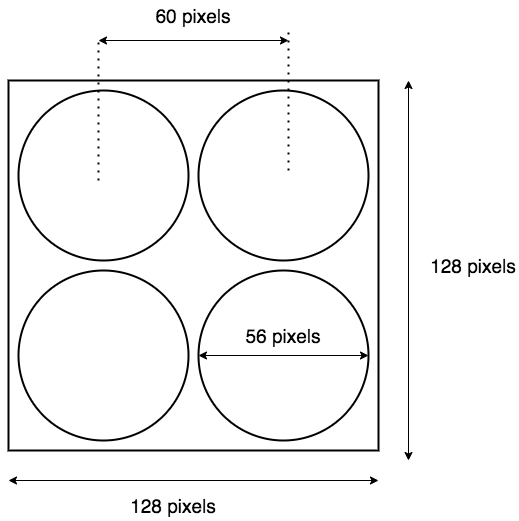
\includegraphics[width=.5\textwidth]{Chapter Materials/Chapter Three Materials/MagAOXpupils.png}
    \caption{Diagram of the desired pupil layout on the OCAM$2$K detector produced by the PWFS. The pupils fall on a gril of 128 by 128 pixels, each pixel having a size of 48 $\mu m$. Each pupil is designed have a diameter of 56 pixels across, and seperated by 60 pixels center to center.}
    \label{fig:PWFSpupils}
\end{figure}
    
The tolerance on the pupil sizes is 1/10$^{th}$ of a pixel, which is 2.4 $\mu m$. Due to the tight tolerances on pupil size, and the large bandpass of the system a custom achromatic triplet lens was designed as the camera lens for the MagAO-X PWFS. The triplet lens allows for the minimization of spherical aberration by allowing for the reduction in curvature of each lens in the triplet, while maintaining the effective focal length needed to meet the magnification requirements. Transverse spherical aberration, which causes a difference in magnification as function of aperture is important to mitigate in this system, because the size of each pupil needs to be uniform. Similarly, lateral chromatic aberration needs to be controlled, because the size of the pupils cannot vary over the bandpass.
	
	
\subsection{Pyramid Design}
MagAO-X will uses an excellent achromatic pyramid with a 5 $\mu m$ tip. The pyramid used in the PWFS is a double pyramid, consisting of two four sided prisms aligned back to back. Details of the design done by \cite{tozzi2008double} are summarized here. A picture of the pyramid is shown in Figure \ref{fig:pyramid}. The total deviation angle needed for the pyramid wavefront sensor is hard to manufacture. Combining two pyramids makes the polishing process easier and at the same time allows us to control chromatic aberrations by using two different glass types. The glass types were chosen using an I.D.L. optimization routine that selected glass combinations from the Shott and Ohara catalog that would give a suitable deflection angle of the double pyramid. The front prism is made from Shott N-SK11, $n_d=1.56384$ and $\nu_D=60.80$, and the back prism is made from Schott N-PSK53, $n_d=1.61800$ and $\nu_D=63.39$. The full diagram of the achromatic double pyramid is found in Figure \ref{fig:fullpyramidprism}.




	
\begin{figure}[h]
	\centering
	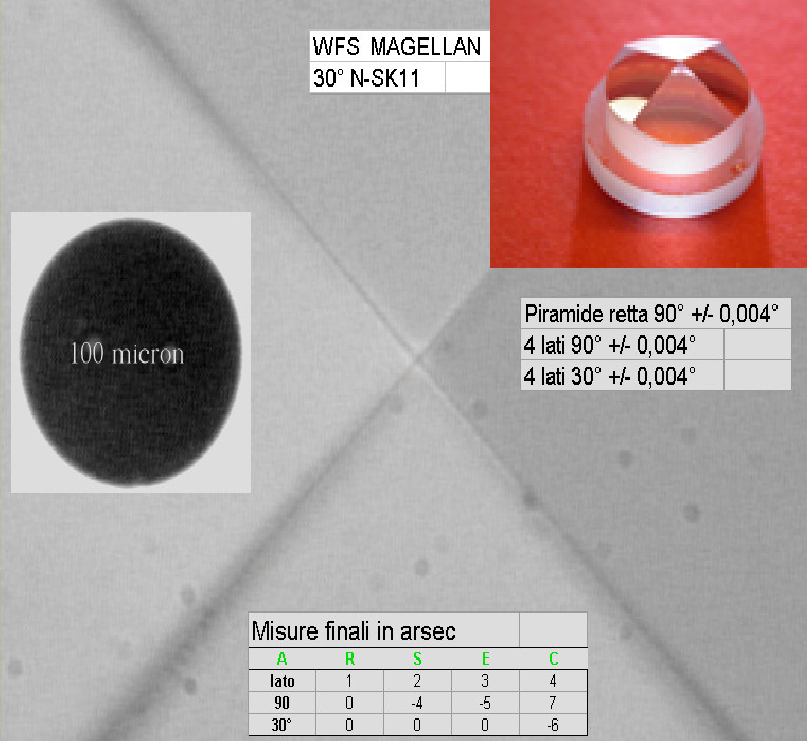
\includegraphics[width=.5\textwidth]{Chapter Materials/Chapter Three Materials/pyramid.png}
	\caption{Fabricated pyramid made in Arcetri, Italy by Paolo Stefanini.}
	\label{fig:pyramidprism}
\end{figure}
	
\begin{figure}
    \centering
    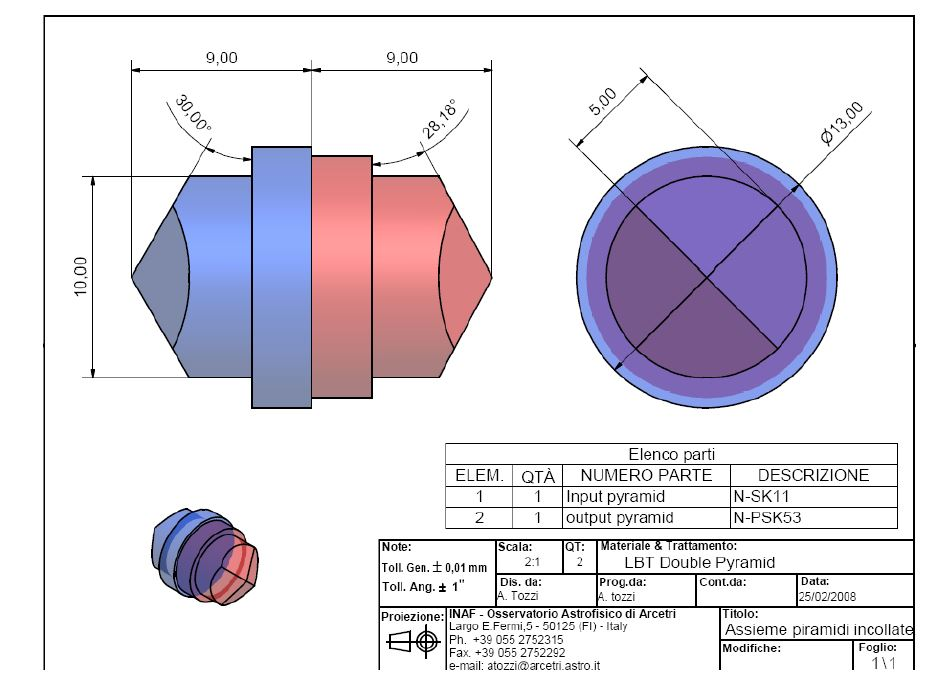
\includegraphics[width=.6\textwidth]{Chapter Materials/Chapter Three Materials/pyramidprismfull.JPG}
    \caption{Drawing of the optical design of the MagAO-X achromatic double pyramid. The pyramid has a high precision entrance pyramid (in blue) made of N-SK11 glass. The exit pyramid (in red) is made of N-PSK53 glass. The angles of the pyramid are designed so that the total deviation of the pair is small.}
    \label{fig:fullpyramidprism}
\end{figure}
	
	
	
\subsection{Wavefront Sensor Design}
	
A design of the wavefront sensor was done in Zemax OpticStudio. An F/69 beam created by an off-axis parabolic (OAP) mirror is focused onto the pyramid tip. A custom achromatic triplet then images four pupils onto our OCAM$^2$K wavefront sensor camera. A layout of the wavefront sensor optical path done in both Zemax and SolidWorks is shown in Figure \ref{fig:oplayout}. We reuse the same off axis parabolic mirror seen by the coronagraph arm of MagAO-X. The double pyramid was modeled by the Arcetri team, (\cite{tozzi2008double}). A custom achromatic triplet was designed to give the correct pupil size and separation. The two windows in the OCAM$^2$K detector are included in the design for completeness. The expected pupil footprint on the image plane for 800 nm wavelength is given in Figure \ref{fig:footprint}. Restraints were placed in the merit function to limit the path length of the PWFS. 

\begin{figure}[h]
	\centering
	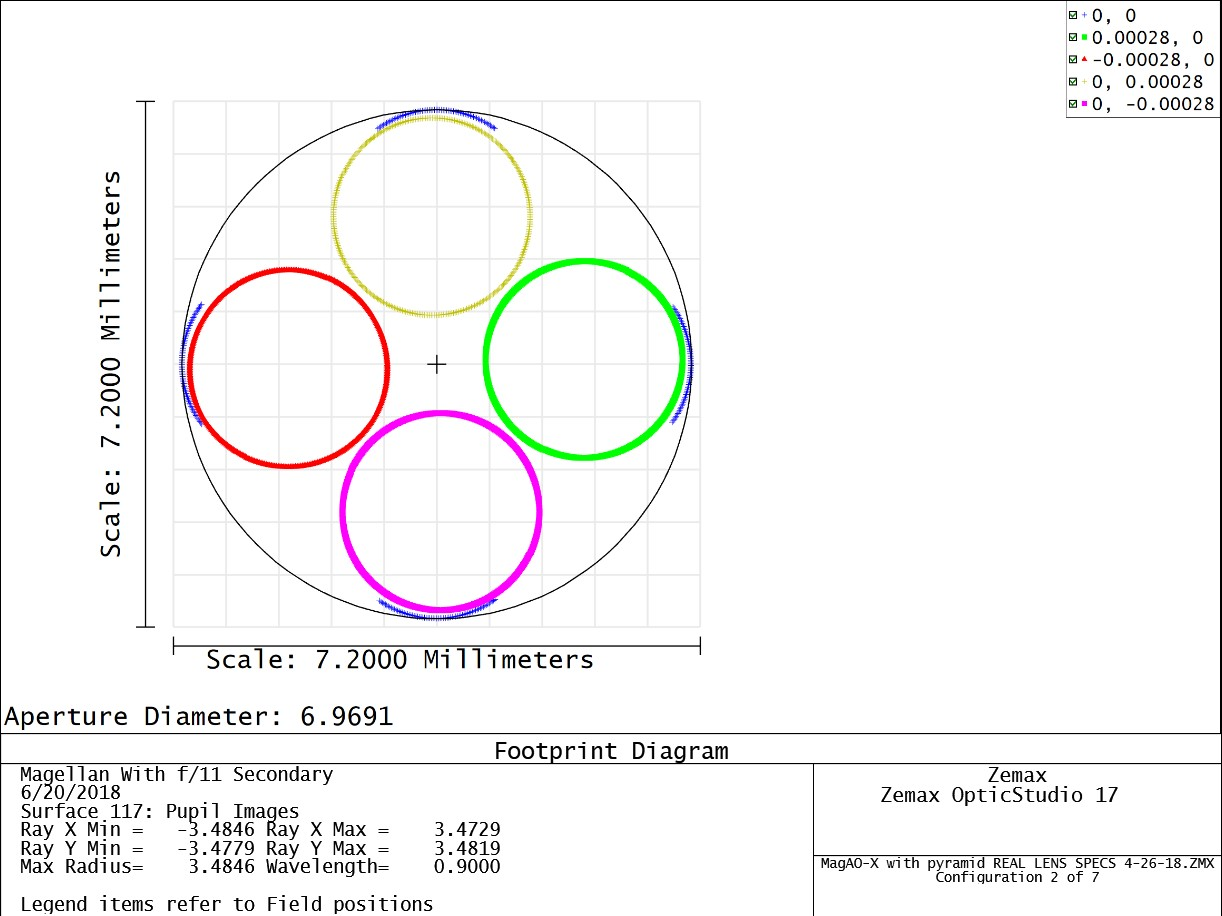
\includegraphics[width=.5\textwidth]{Chapter Materials/Chapter Three Materials/Pupils6-20-18.jpg}
	\caption{Beam footprint diagram at the image plane. Each colored circle is a pupil.}
	\label{fig:footprint}
\end{figure}

\begin{figure}
    \centering
    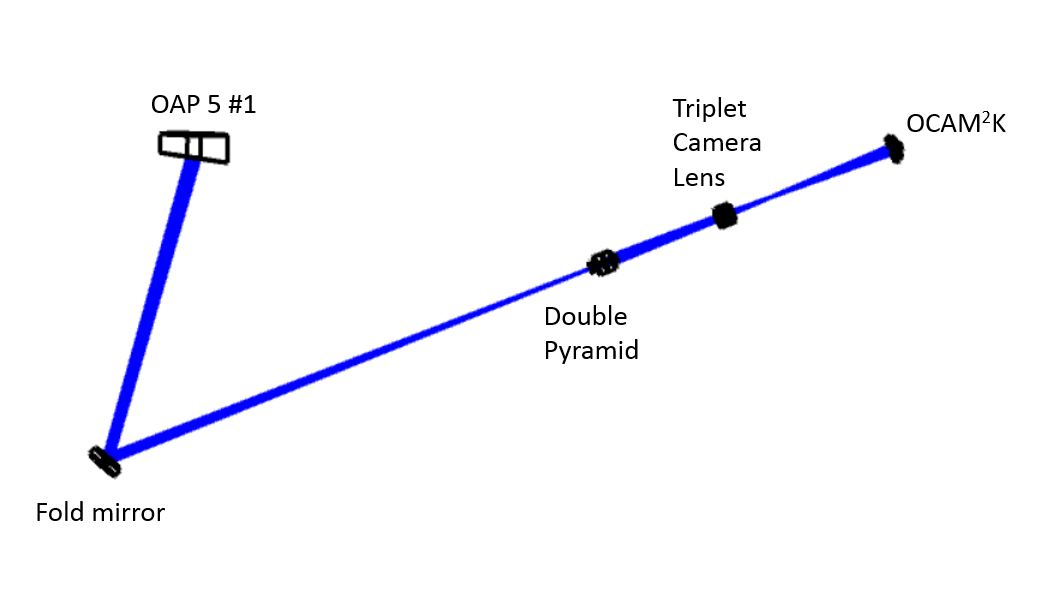
\includegraphics[width=.8\textwidth]{Chapter Materials/Chapter Three Materials/layout.jpg}
    \caption{Optical path of the PWFS in Zemax. The 5$^{th}$ OAP mirror forms an F/69 focus on the tip of the double pyramid. The triplet camera lens images the pupils onto the OCAM$^2$K camera.}
    \label{fig:my_label}
\end{figure}

\begin{figure}
    \centering
    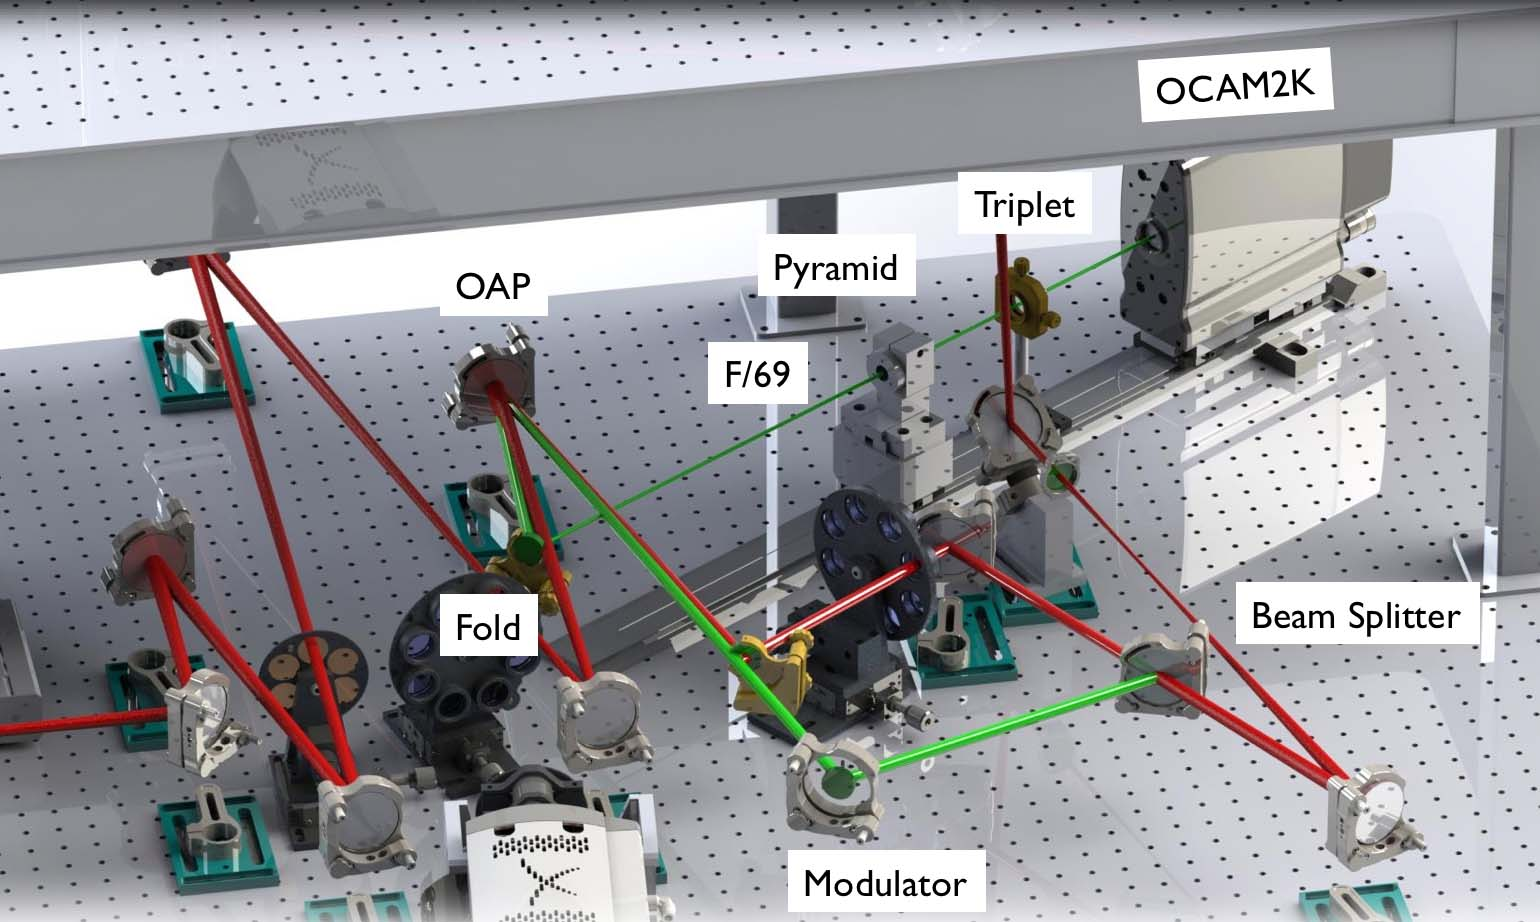
\includegraphics[width=.8\textwidth]{Chapter Materials/Chapter Three Materials/PWFSOptoMech.jpg}
    \caption{Layout of the pyramid wavefront sensor (green path) on the MagAO-X optical bench, (\cite{close2018optical}). The Zemax ray trace was imported into SolidWorks for the optomechanical design. The red-light path is the science path that goes to the coronagraph.}
    \label{fig:oplayout}
\end{figure}
	
	
	
	
\subsection{Achromatic Triplet Design}

The size and separation of the pupils on the detector directly affects the performance of the PWFS. If the pupils are undersized, there will be aliasing in reconstruction of the higher order modes. If the separation between pupils is not correct, complications will arise when pixels are binned on the detector to change the pupil sampling and the integration time.  To ensure the correct size and separations a custom achromatic triplet was designed in Zemax. A schematic of the lens is shown in Figure \ref{fig:triplet}. 


\begin{figure}[h]
	\centering
	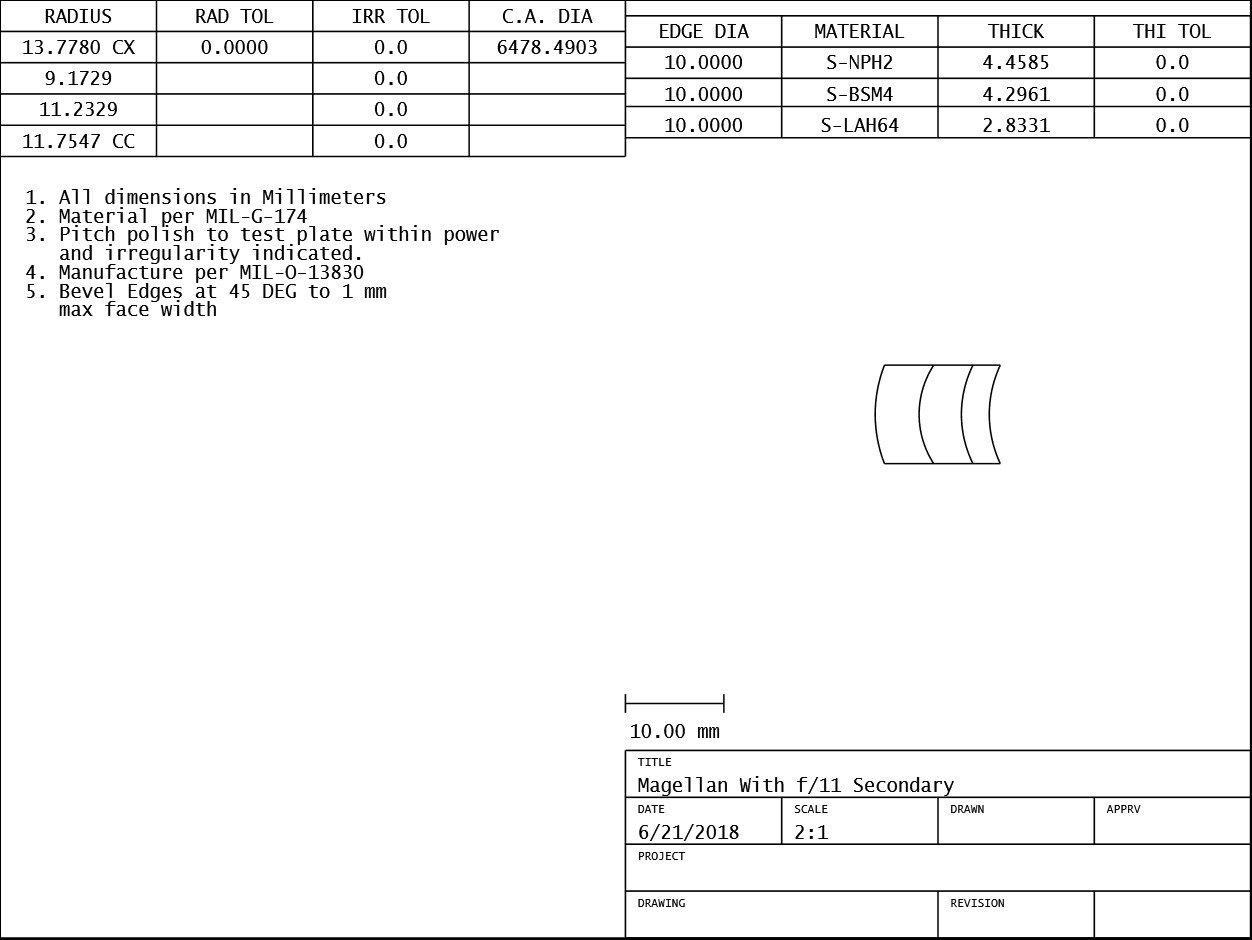
\includegraphics[width=.8\textwidth]{Chapter Materials/Chapter Three Materials/cameralenstripletSPEC.jpg}
	\caption{Lens schematic of the achromatic triplet in zemax. The radius of curvatures of each surface are listed under the Radius column. The material and thickness of each lens is given in under Material and Thick columns.  }
	\label{fig:triplet}
\end{figure}


In the optimization merit function restraints were place to insure that the triplet was manufacturable, and met our system requirements. The thickness at the middle and edges of each of the lenses in the triplet were constrained to insure that the lens was of reasonable curvature and the system did not converge to an impossible shape. The main focus of the merit function was to insure that the pupil sizes and separations were the same as a function of field and wavelength. This was done by calculating coordinates of the edges of the pupils using real ray tracing operands, and then using math operands to use the coordinates to calculate pupil size and spacing. Targets for the size and spacing were then set to the desired values, and a large weight was applied to each of these operands to force the system to converge to our desired outcome.


%%%%% Go in and show a photo of the merit function?
	
A tolerance analysis to determine lens performance as a function of wavelength is done using parameters from the Precision grade Optimax manufacturing tolerancing chart. Reasonable values of alignment errors were estimated and included in the tolerancing analysis. The figure of merit used was the RMS angular radius of the lens because the pyramid is an afocal system. A 500 trial Monte Carlo simulation was done for three wavelengths, 600nm, 800nm, and 1000nm. At each wavelength the nominal, mean, and worst RMS angular size (twice the angular radius) was recorded. The difference of the mean and worst angles with respect to the nominal value was calculated. That change in angle was propagated through the system to estimate the change in size we would expect. The propagation is shown in Figure \ref{fig:propagation}, where $\theta_n$ is the nominal RMS angular size, and $\theta_\Delta$ is the change in RMS angular size we use to calculate the estimated change $\Delta y$. The distances $x_1 ... x_5$ were taken from the Zemax design, and the indexes $n_1, n_2, n_3$ correspond to air, BK-7, and Sapphire respectively. The index of refraction was adjusted for the different wavelengths when the propagation was calculated using trigonometry and Snell's law. The results are summarized in Figure \ref{fig:change}, where the change in size in nanometers is graphed against wavelength. At worst we expect about a 45 nm change in pupil size and separation, but no change on average. Both are well within our tolerance of the change being no greater than 1/10th a pixel, or 2.4$\mu$m.
	
	
	
\begin{figure}[h]
	\centering
	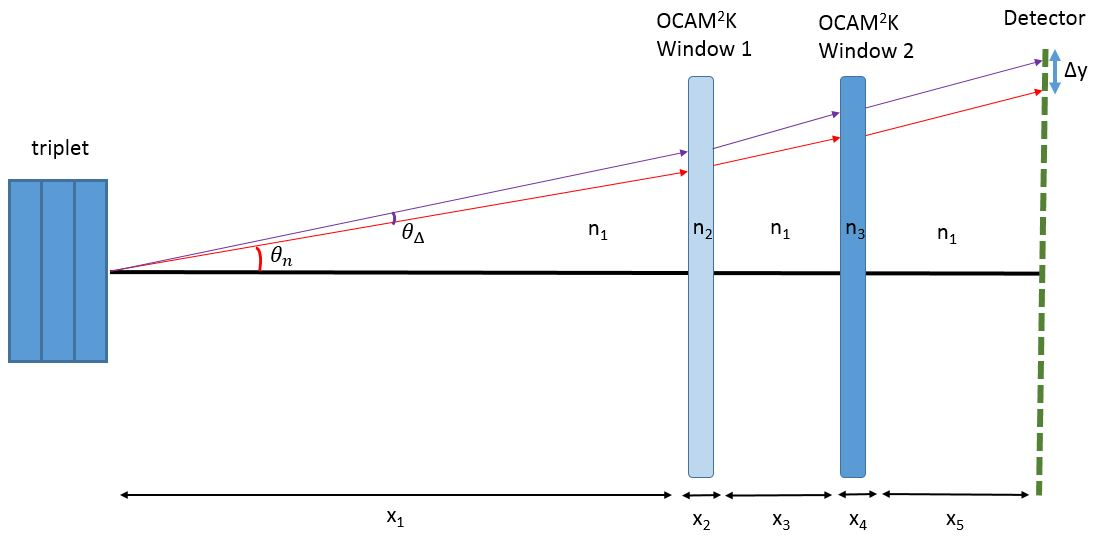
\includegraphics[width=.8\textwidth]{Chapter Materials/Chapter Three Materials/propagation.JPG}
	\caption{Diagram of the light propagation path used to calculate the change in pupil size. Light is propogated from surface to surface using paraxial ray tracing and Snell's law.}
	\label{fig:propagation}
\end{figure}
	
	
\begin{figure}[h]
	\centering
	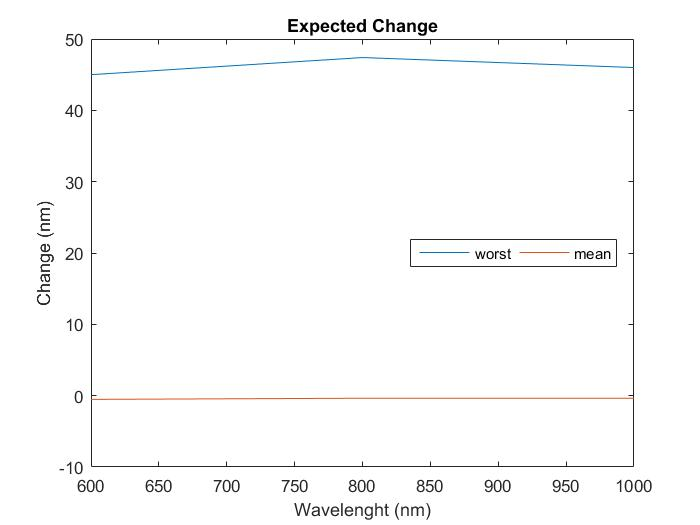
\includegraphics[width=.5\textwidth]{Chapter Materials/Chapter Three Materials/achromaticchangegraph.jpg}
	\caption{Expected change in pupil size as a function of wavelength.}
	\label{fig:change}
\end{figure}
	
\section{System Performance}
	
A simulation of the expected partial illumination of pupil pixels was done in MATLAB. A binary model of the MagAO-X pupil was generated with 10 times the spatial sampling than our expected PWFS pupil. We then bin it down to the expected pupil sampling of our PWFS. That is, we start with a pupil of 560 by 560 pixels, and bin down to a 56 by 56 pixel pupil by summing 10 by 10 pixel bins and normalizing. The expected illumination pattern is shown in Figure \ref{fig: pupilpixels}. A table of the pixel counts is given in Table \ref{tab:actuators}. We expect 1958 fully illuminated pixels within our pupil. 
	
	
\begin{figure}%
	\centering
	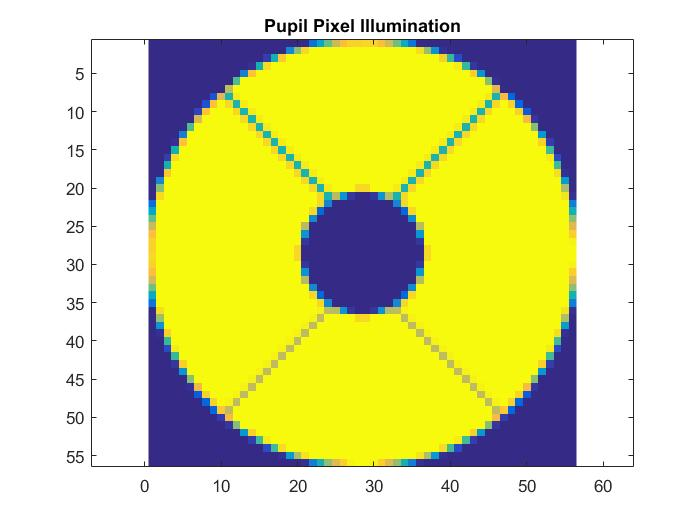
\includegraphics[width=.4\textwidth]{Chapter Materials/Chapter Three Materials/pupilpixels.jpg}
	\caption{Expected pupil illumination on the PWFS.}	
	\label{fig: pupilpixels}
\end{figure}
	
	
	
\begin{table}[h]
	\begin{center}       
		\begin{tabular}{|l|l|} %% this creates two columns
				%% |l|l| to left justify each column entry
				%% |c|c| to center each column entry
				
				\hline%% use of \rule[]{}{} below opens up each row
				\rule[-1ex]{0pt}{3.5ex} $\%$ \textbf{Illumination} & \textbf{$\#$ of Pixels }  \\
				
				\hline%% use of \rule[]{}{} below opens up each row
				\rule[-1ex]{0pt}{3.5ex} 100$\%$ & 1958  \\
				\hline%% use of \rule[]{}{} below opens up each row
				\rule[-1ex]{0pt}{3.5ex} 90$\%$ & 166  \\
				\hline%% use of \rule[]{}{} below opens up each row
				\rule[-1ex]{0pt}{3.5ex} 80$\%$ & 24  \\
				\hline%% use of \rule[]{}{} below opens up each row
				\rule[-1ex]{0pt}{3.5ex} 0$\%$ & 46  \\
				\hline%% use of \rule[]{}{} below opens up each row
				\rule[-1ex]{0pt}{3.5ex} 60$\%$ & 20  \\
				\hline%% use of \rule[]{}{} below opens up each row
				\rule[-1ex]{0pt}{3.5ex} 50$\%$ & 18  \\
				\hline%% use of \rule[]{}{} below opens up each row
				\rule[-1ex]{0pt}{3.5ex} $<$ 50$\%$ & 904  \\
				\hline
		\end{tabular}
	\end{center}
	\caption{Percentage of illuminated pixels one of the 56 by 56 pixel pupils. }
	\label{tab:actuators}
\end{table}
	
\section{Initial Results}
	
The camera triplet was manufactured by Rainbow optics and the as-built specifications of the lens was incorporated into the Zemax design. The tolerance of our system was that the pupil size and separation would be within 1/10$^{th}$ of a pixel. We found that our fabricated lens was slightly under specifications. The pupils are slightly oversized, and the pupil separation is too close together. Table \ref{tab:asbuilt} shows the system requirements of the MagAO-X system, and the expected performance with our fabricated lens. The lens was mounted in a piezo-motorized stage shown in Figure, that allowed for X-Y positioning, as well as rotation. 
	
	
\begin{table}
	\begin{center}
		\begin{tabular}{ | l| l |  l |}
			\hline
			\textbf{Parameter}& \textbf{Requirement} & \textbf{As Built}\\ \hline
			Wavelength Range &600- 1000 nm& 600-1000 nm\\ \hline
			Pupil Size & 56 pixels; 2.688 mm& 2.696 mm\\ \hline
			Pupil Separation & 60 pixels; 2.880 mm& 2.857 mm \\ \hline
			Pupil Tolerances & $\Delta$ $<$ 1/10th pixel; 2.4 $\mu$m& $\Delta_{size}$=8 $\mu m$,  $\Delta_{sep}$=-23 $\mu m$ \\ \hline
			Lens Diameter & 10 mm $<$ D  $<$ 20 mm & D= 10.1 mm\\ \hline
				
		\end{tabular}
	\end{center}
	\caption{Parameters for the MagAO-X pyramid wavefront sensor and the as built expected performance from our Zemax model.}
	\label{tab:asbuilt}
\end{table}



\begin{figure}
    \centering
    \includegraphics[width=.8\textwidth]{Chapter Materials/Chapter Three Materials/cameraLensPiezoHolder.png}
    \caption{The custom achromatic triplet lens mounted in a precision X-Y lens mount.}
    \label{fig:mountedtriplet}
\end{figure}
	
An initial alignment of the MagAO-X pyramid wavefront sensor was done using a HeNe single mode fiber laser, two off axis parabolic mirrors, and a temporary pupil mask with coarse edges. The pyramid optic, camera lens, and OCAM$^2$K were mounted on a coaxial rail system from ThorLabs as shown in Figure \ref{fig:mountedPWFS}. Custom mounting plates were fabricated for each optic, so that each could be mounted onto rail carriages and meet the beam height requirement of 5 inches from the optical table. 

\begin{figure}
    \centering
    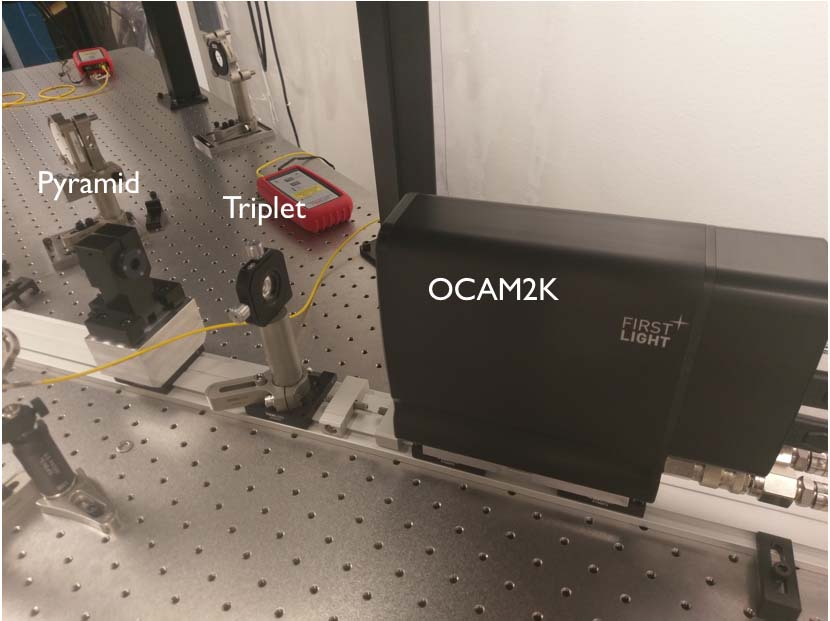
\includegraphics[width=.8\textwidth]{Chapter Materials/Chapter Three Materials/mountedPWFS.jpg}
    \caption{The mounted pyramid optics, camera lens, and OCAM$^2$K camera on a coaxial rail from ThorLabs.}
    \label{fig:mountedPWFS}
\end{figure}

The mount of the pyramid optic has a custom target that aligns with the pyramid tip. To align the PWFS we first mounted the pyramid optic with the target on the optical rail and placed it on the MagAO-X optical table. The position of the rail and the tip/tilt of the incoming beam from OAP $\#5$, was adjusted iteratively until the beam hit the center of the target when the pyramid was placed at both the front and the back of the rail. This established the beam line for the system. The camera lens and OCAM$^2$K was then placed on the rail according to the Zemax design. The fine focus of the pyramid optic was dialed using a micrometer nudger, and by examining the signal of the pyramid pupils with and without modulation. The spacing of the camera lens and the OCAM$^2$ were adjusted until the size and separation of the pupils were in specifications. The measurement of the pupil parameters was done by a circle fit of the modulated pyramid pupils shown in Figure \ref{fig:fitPupils}. The average size of the MagAO-X pupils is 55.83 pixels in diameter. Figure \ref{fig:MagAOXpupils} shows the white light pupils of the MagAO-X PWFS under 5 $lambda/D$ modulation.

\begin{figure}
    \centering
    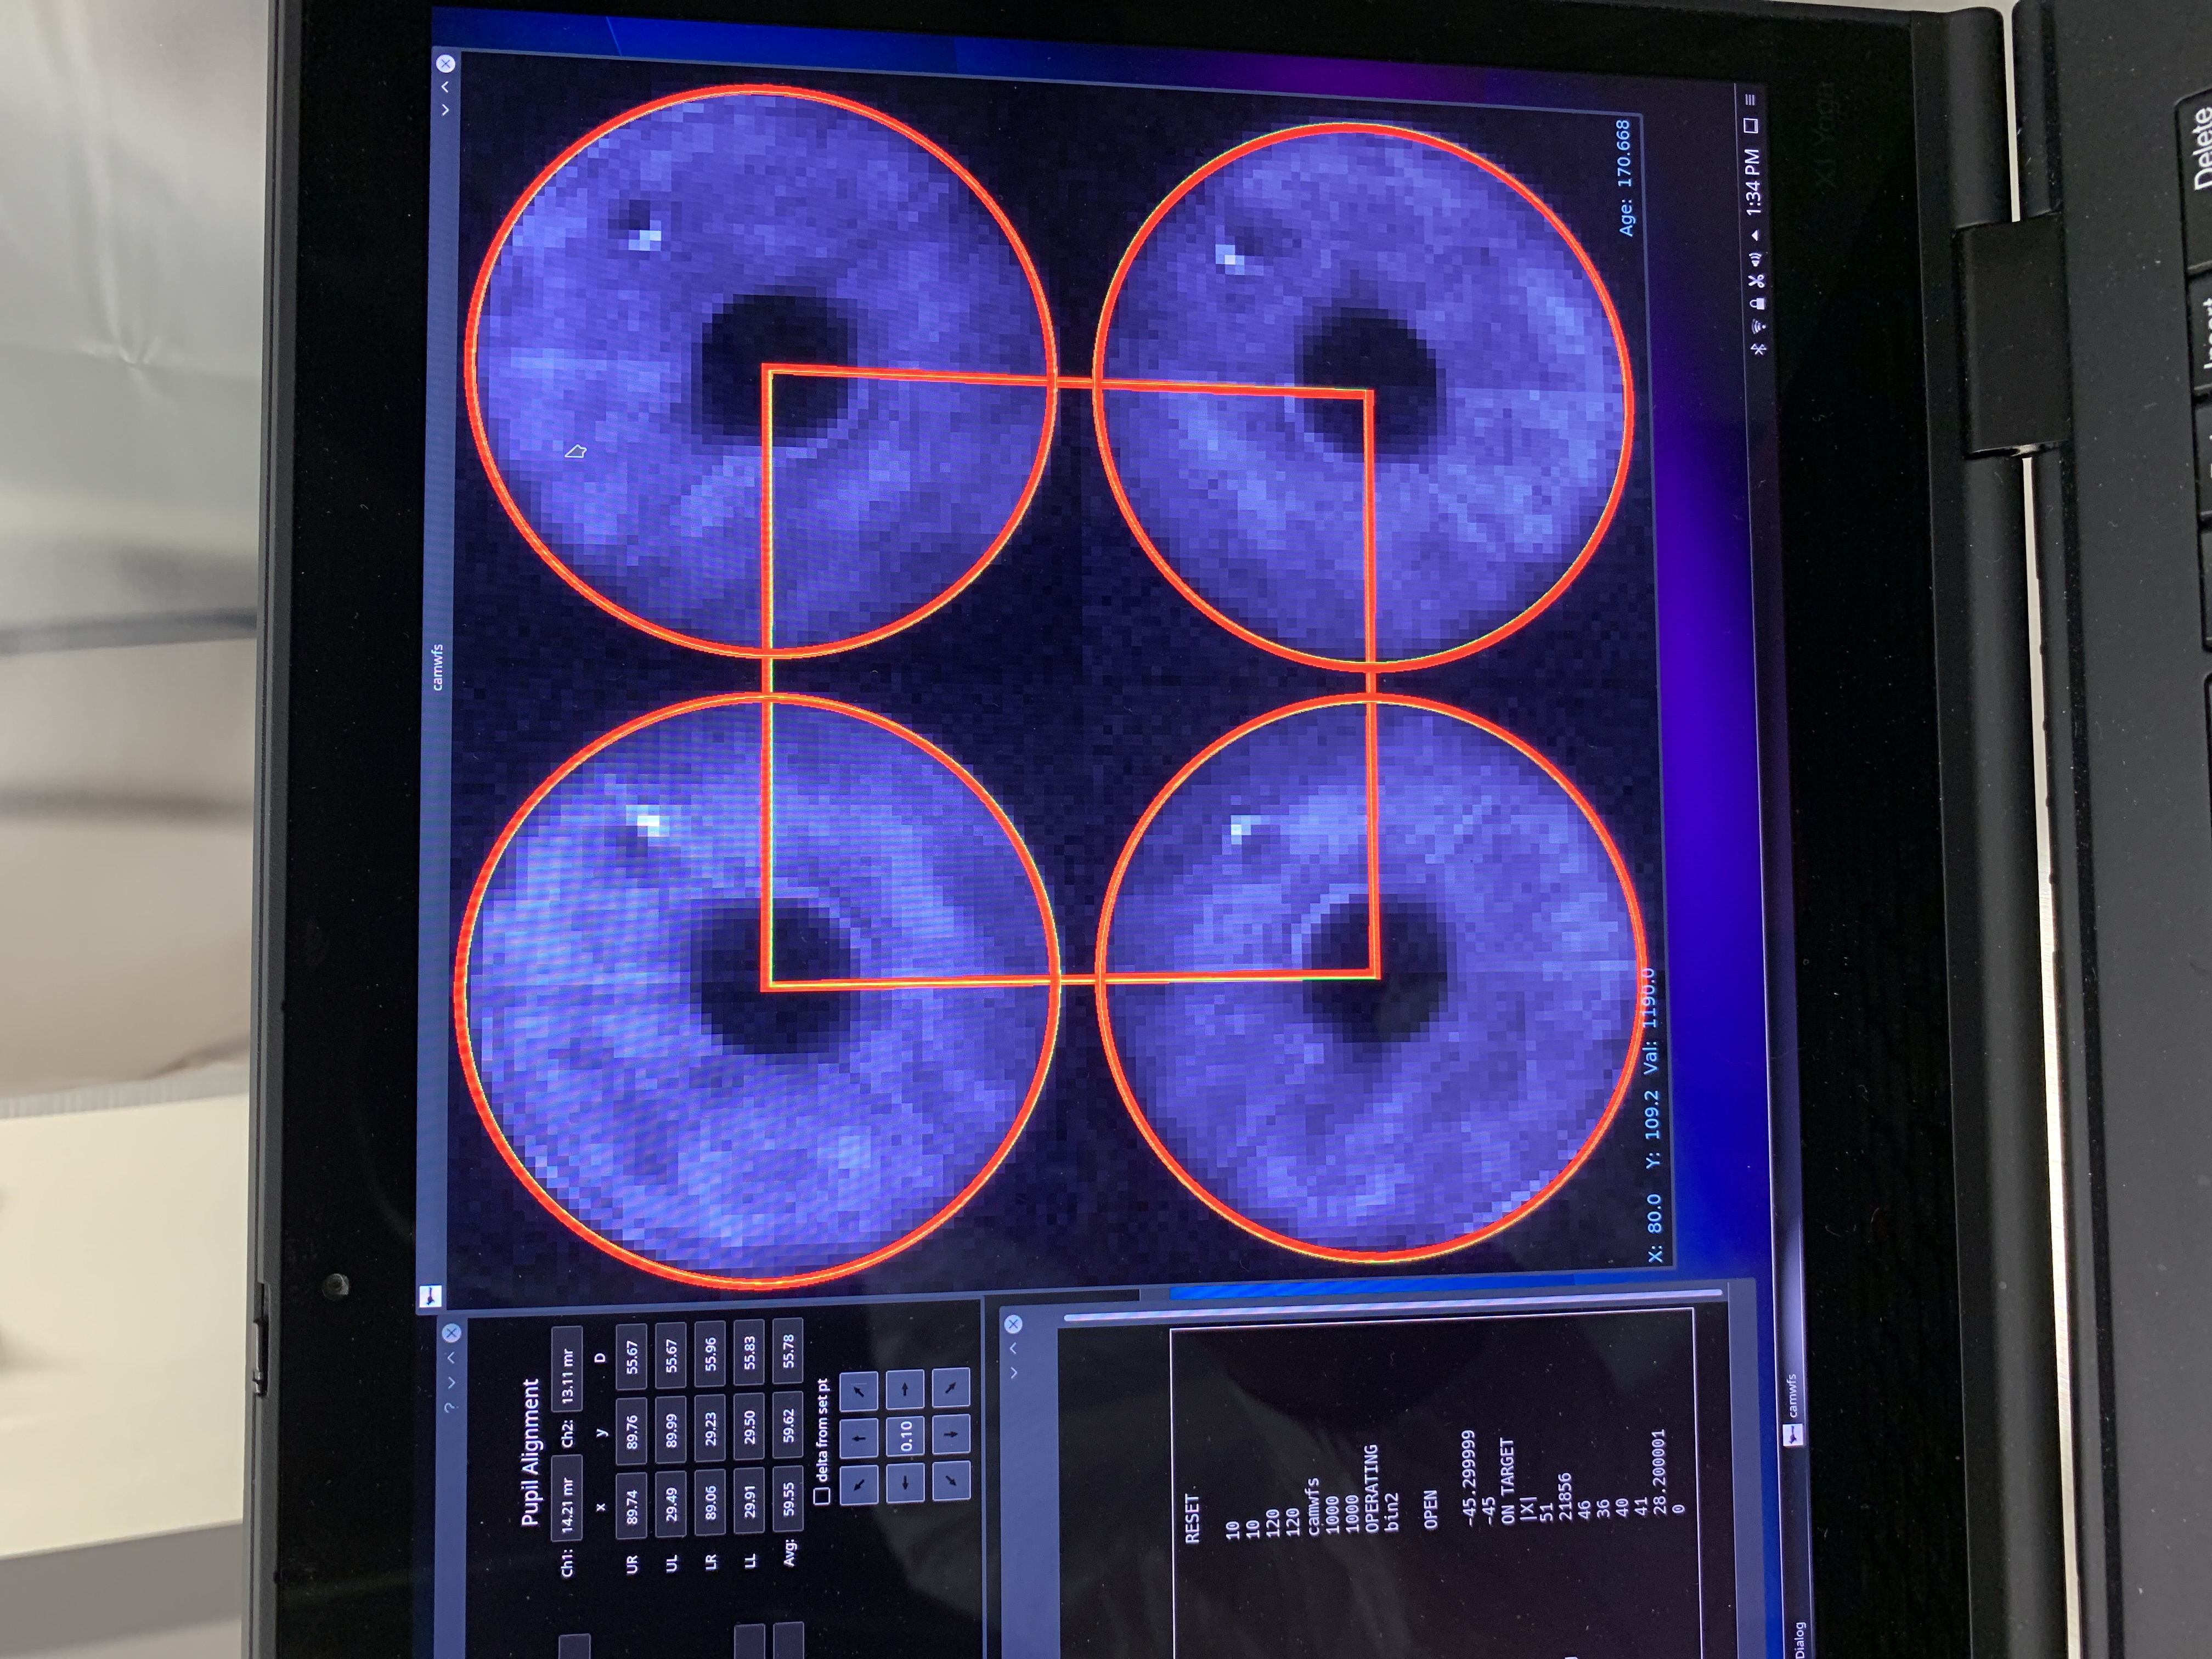
\includegraphics{Chapter Materials/Chapter Three Materials/Age 170.668.jpeg}
    \caption{Caption}
    \label{fig:fitPupils}
\end{figure}

\begin{figure}
    \centering
    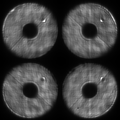
\includegraphics{Chapter Materials/Chapter Three Materials/MagAOXpupil5LD.png}
    \caption{The MagAO-X pyramid wavefront sensor pupils with 5 $\lambda/D$ modulation. The spiders and central obscuration are from the aperture of the Magellan Telescope.  }
    \label{fig:MagAOXpupils}
\end{figure}
\chapter{Analysis of the Pyramid Wavefront Sensor Signals}\label{CH3}
%Babcock. Summary of some on sky systems. 

A key component of an ExAO system is the wavefront sensor, which measures aberrations from atmospheric turbulence. A common choice of WFS in current and next generation instruments is the pyramid wavefront sensor (PWFS). The PWFS is a highly sensitive wavefront sensor that is able to measure the wavefront at high speeds. The sensitivity and linear range of the PWFS can be tuned by dynamic modulation, making the PWFS robust to different seeing conditions. 


\section{The Pyramid Wavefront Sensor}\label{PWFSintro}
The optical design of the PWFS consists of four components: a focusing optic, the glass pyramid, and a relay lens to image the pupils on the detector \citep{ragazzoni2002pyramid}. Figure \ref{fig:pyramid} shows a schematic of the operation of a PWFS \citep{shatokhina2014fast}.  The starlight is first brought to a focus on the tip of a glass pyramid that splits the focal plane into parts. The apex angle of the pyramid imparts a tilt to separate each of the sections. The result is copies of the telescope pupil that are separated spatially on a detector. The number of pixels across each pupil determines the number of modes the instrument is sensitive to. Current on-sky adaptive optics systems that have a PWFS use a four-sided PWFS. The Magellan Adaptive Optics System (MagAO) \citep{close2018status}, the Large Binocular Telescope Interferometer (LBTI) \citep{esposito2011adaptive}, and MagAO-X use an achromatic double four-sided pyramid. The SCExAO instrument uses two crossed roof prisms as its pyramid optic. The basic PWFS is highly sensitive but suffers from low dynamic range. A modulator is used to move the beam around the pyramid tip to increase the linear range of the PWFS. Modulation is achieved by oscillating a piezo-actuator driven mirror to drive the PSF on the pyramid tip into a circular pattern with a radius quoted in units of $\lambda/D$, where $\lambda$ is wavelength, and $D$ is the diameter of the entrance pupil. This increases the effective spot size on the pyramid tip which increases the sensor's linearity at the cost of sensitivity \citep{guyon2005}.  

\begin{figure}
    \centering
    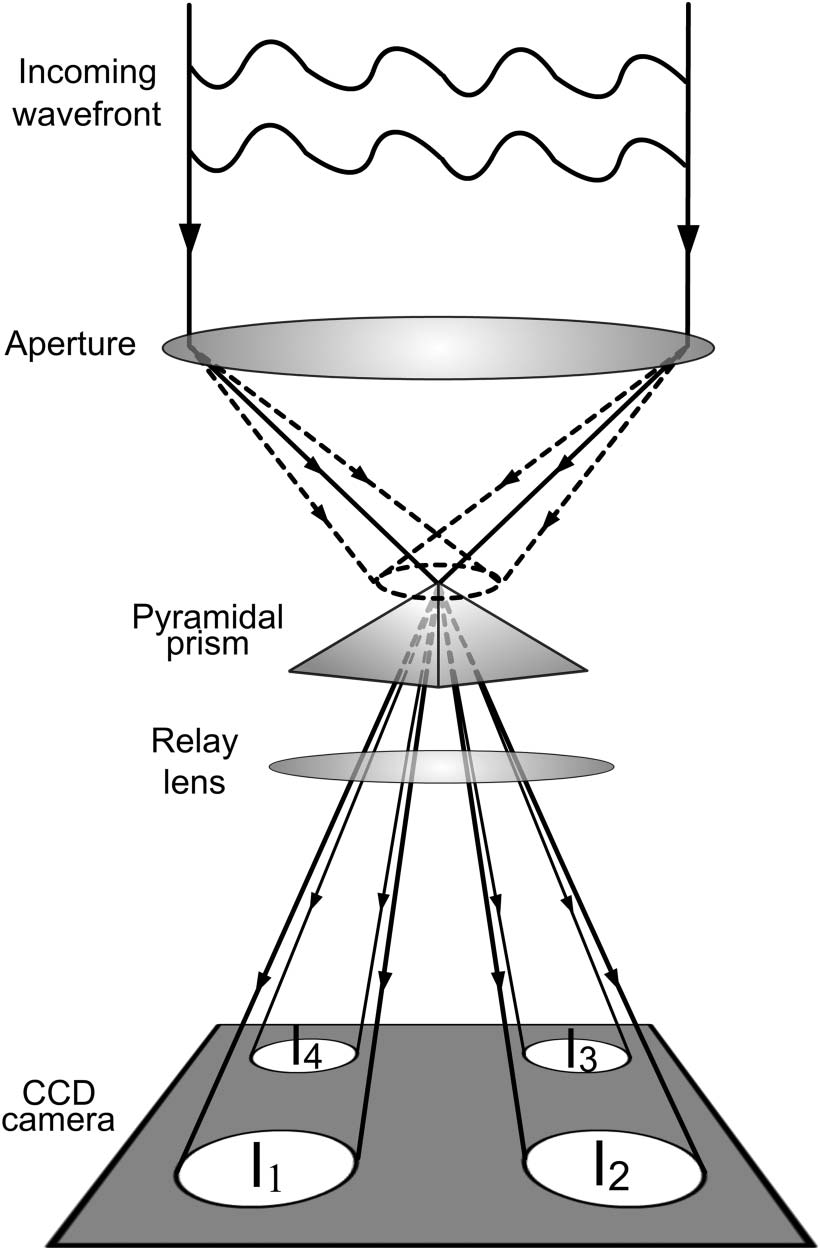
\includegraphics[width=0.75\textwidth]{Chapter Materials/Chapter Three Materials/pyramidDiagram.jpg}
    \caption{Optical design of a PWFS. Light from the telescope is focused onto a glass pyramid tip where it is split and then the pupil plane is reimaged onto a detector. The result is copies of the telescope pupil that contain intensity fluctuations that are related to the wavefront phase \citep{shatokhina2014fast}.}
    \label{fig:pyramid}
\end{figure}


The intensity measured in the PWFS must be processed to infer the wavefront phase. First, the image is dark subtracted and gain corrected to remove detector artifacts. A threshold mask is then applied to mask out any pixels that do not contain a signal. The wavefront sensor response to a flat wavefront is subtracted off to leave only the intensity pattern caused by the wavefront phase error. The intensity in the pupils can be combined to estimate the wavefront derivative, or slope. We refer to this as the Slopes Maps (SM) calculation. The equation for the 4PWFS is,


\begin{eqnarray}
    S_x=\frac{I_1+I_2-I_3-I_4}{I_1+I_2+I_3+I_4}     \label{4PWFSslopes} \\
    S_y=\frac{I_1-I_2-I_3+I_4}{I_1+I_2+I_3+I_4} \nonumber
\end{eqnarray}

where $S_x, S_y$ are the local wavefront slopes in the x and y direction, and $I_1...I_4$ are the intensity values of the pixel corresponding to the same location in each pupil. The intensity patterns in the pyramid pupils contain both the X and Y spatial information of wavefront gradient from the diffraction off of the pyramid edges. The Raw Intensity (RI) signal processing method uses the pyramid signal as-is. The same processing steps are performed: masking, dark subtraction, and gain correction. The resulting signal is unraveled into a single vector of intensity signals. The benefit of the Raw Intensity method is that it is relatively unaffected by alignment errors. The major challenge in using this technique is obtaining a good flat wavefront reference image. The signals in the pyramid pupils are then extracted into a single column vector of intensity values.

All current PWFS on telescopes use a 4PWFS. ExAO systems need high sampling of the PWFS pupils to optimize performance, and as a result require larger detectors. Detector size, speed, and noise all impose limits on wavefront sensor designs and limit the performance of an GSMT-ExAO system. We are interested in exploring the 3PWFS as an alternative PWFS for an ELT-ExAO wavefront sensor to overcome these limitations. The 3PWFS only has three copies of the pupil and therefore uses fewer detector pixels than the 4PWFS and should be less sensitive to read noise. We assess the performance of the 3PWFS compared to the 4PWFS in simulation to determine if the 3PWFS does outperform the 4PWFS when using high read noise detectors.

To assess the performance of the 3PWFS compared to the 4PWFS, a simulation was developed using the Object Oriented Matlab Adaptive Optics toolkit (OOMAO) \citep{OOMAO}. The OOMAO toolkit is an end-to-end adaptive optics model that can simulate different combinations of guide stars, turbulent atmospheres, wavefront sensors, deformable mirrors, and science cameras. Light is propagated using Fraunhofer diffraction. The PWFS is simulated using a single tip/tilt phase mask that is segmented into N parts. Figure \ref{fig:oomaoFigs}.A and \ref{fig:oomaoFigs}.C show the masks for the 3PWFS and 4PWFS. The masks are scaled and rotated according to a user input for rotation and pyramid apex angle that controls the separation of the pyramid pupils. After scaling, the mask is converted into a phase mask that is applied at the focal plane to simulate a pyramid tip. Figure \ref{fig:oomaoFigs}.C and \ref{fig:oomaoFigs}.D show the resulting pyramid pupils on the simulated wavefront sensor camera, using a flat wavefront and 5 $\lambda/D$ modulation. The master OOMAO toolbox simulates a 4PWFS using Slopes Maps. We extended the PWFS class in OOMAO to include a 3PWFS, taking care that the amplitude of the tip/tilt phase in the 3PWFS phase screen generation matched that of 4PWFS. We included our derivation of the Slopes Maps equation for the 3PWFS (derived in Section~\ref{SlopesDerivation} below), and added the Raw Intensity method for both the 4PWFS and the 3PWFS. For both the Slopes Maps and Raw Intensity method the signal was normalized by the mean value across all valid pixels on the wavefront sensor detector, instead of normalizing cell by cell. 

\begin{figure}
    \centering
    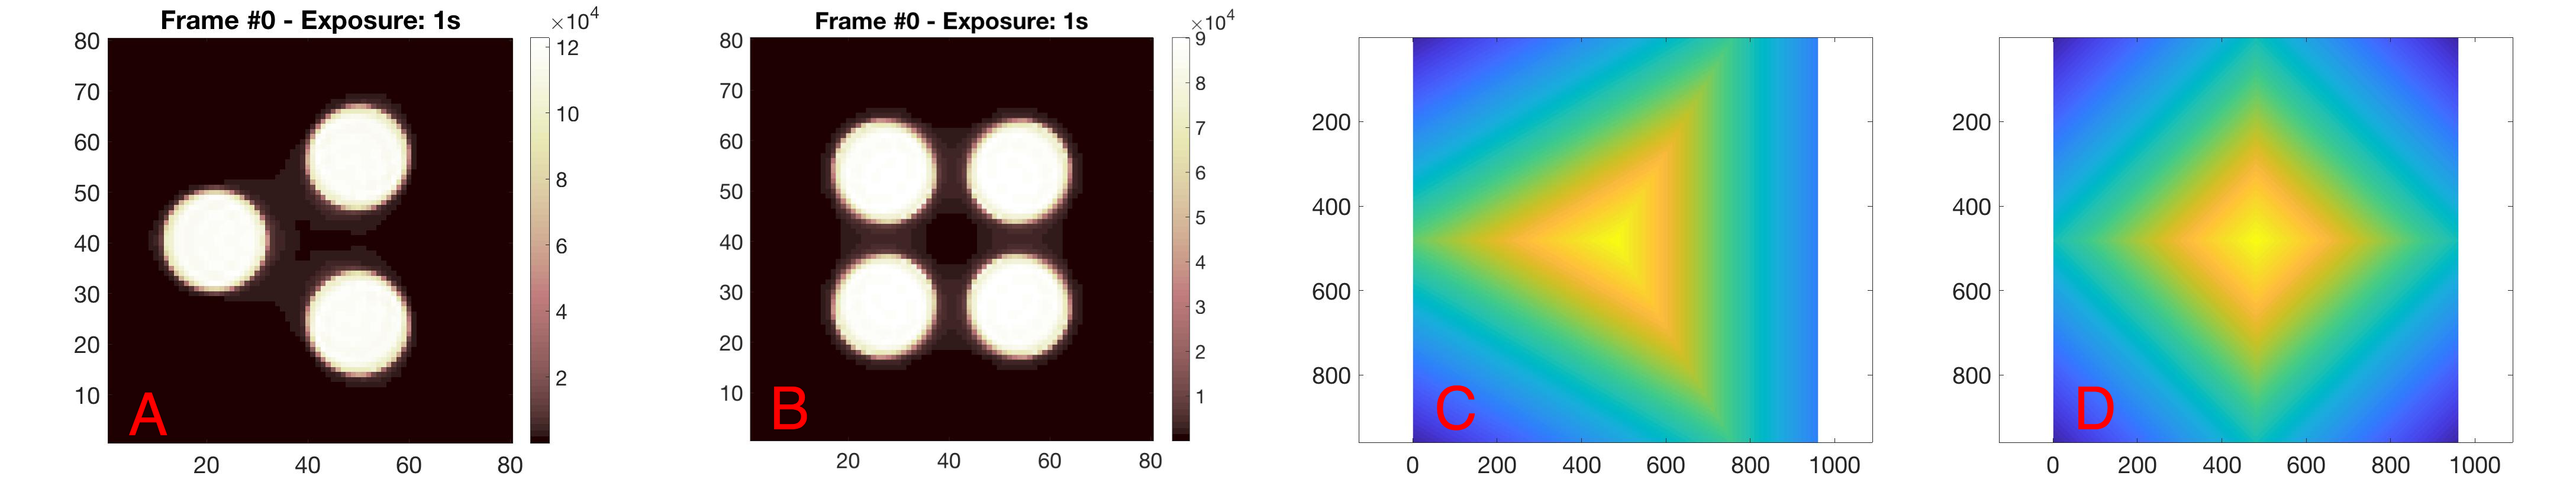
\includegraphics[width=1\textwidth]{Chapter Materials/Chapter Two Materials/oomaoFigs.png}
    \caption{Details of the simulated PWFS in OOMAO. A) and B) The simulated 3PWFS and 4PWFS pyramid masks in OOMAO. These masks are used as a phase screen in the pupil plane to emulate the focal plane splitting and separation done by a real glass pyramid. C) and D) The pupils from the 3PWFS and 4PWFS respectively on the simulated detector. In OOMAO the user can change the size, separation, and intensity values of the pupils through user defined inputs.}
    \label{fig:oomaoFigs}
\end{figure}


\section{Diffraction Theory of the Foucault Test}\label{diffraction}
\subsection{Derivation of Expected Signal from the Foucault Test}
  The PWFS is an extension of the knife edge test: each of the pyramid pupils are the signal from a knife edge test, but include a mirroring effect of the signal across the facets. The underlying physical processes of the pyramid and the knife edge are the same, so we can use the equations that describe the knife edge test explore the operation of the PWFS. The diffraction theory of the PWFS has been studied in detail. \cite{verinaud2004nature} extends the knife edge diffraction theory to model the signal of a roof sensor with dynamic circular modulation. \cite{hutterer2019real} extends the knife edge analysis into general operators such that modulations of any pattern can be modeled. \cite{shatokhina2014fast} presents simplified equations to approximate pyramid signals with and without modulation.\cite{correia2020performance}, and \cite{fauvarque2019kernel} model the pyramid operation as a Fourier filter. In this chapter we use a formalism similar to Vérinaud, but limit our analysis to that of a one dimensional knife edge test for simplicity. We use the knife edge analysis to derive the relationship of the PWFS sensitivity to Fourier modes. Fourier modes have a direct relationship to locations on the focal plane; which is important to coronagraphy because we are trying to maximize the contrast in the dark hole region created by the coronagraph.
 
 In this section we consolidate the diffraction theory of the knife edge test by \citep{linfoot1948theory}, \citep{katzoff1971quantitative}, and \citep{wilson1975wavefront} into a single derivation with uniform notation. Expanding upon their results, we link phase aberrations in the shape of Fourier modes to intensity patterns produced by the knife edge test. We assume a focal plane bisected by a binary amplitude mask representing the knife edge. 
 
 Figure \ref{fig:derivationFlow} describes the steps taken in this derivation. The diagram is in two dimensions for visualization, but in this derivation we assume a one dimensional case for simplicity. We start with an electric field in the entrance pupil, $u_0(x_0)$ that has a phase error given by $\cos(nx)$. A Fourier transform is taken to the focal plane where the knife edge, $H_f(\xi_f)$ is applied. We don't actually solve for $U(\xi_f)$, the electric field in the focal plane, and instead take an inverse Fourier transform to the conjugate pupil plane where the knife edge test signal is found. The electric field at this pupil plane is given by $u(x_i)$, is the convolution of the electric field in the entrance pupil propagated to this pupil plane, $u_0(x_i)$, and the inverse Fourier transform of the knife edge, $h_i(x_i)$. The phase error in the electric field is expanded in a power series, then linearized, and the modulus squared is taken to find the field intensity. By subtracting off the constant term, we are left with the intensity pattern due to only the phase errors. 
 
 
 
 \begin{figure}
     \centering
     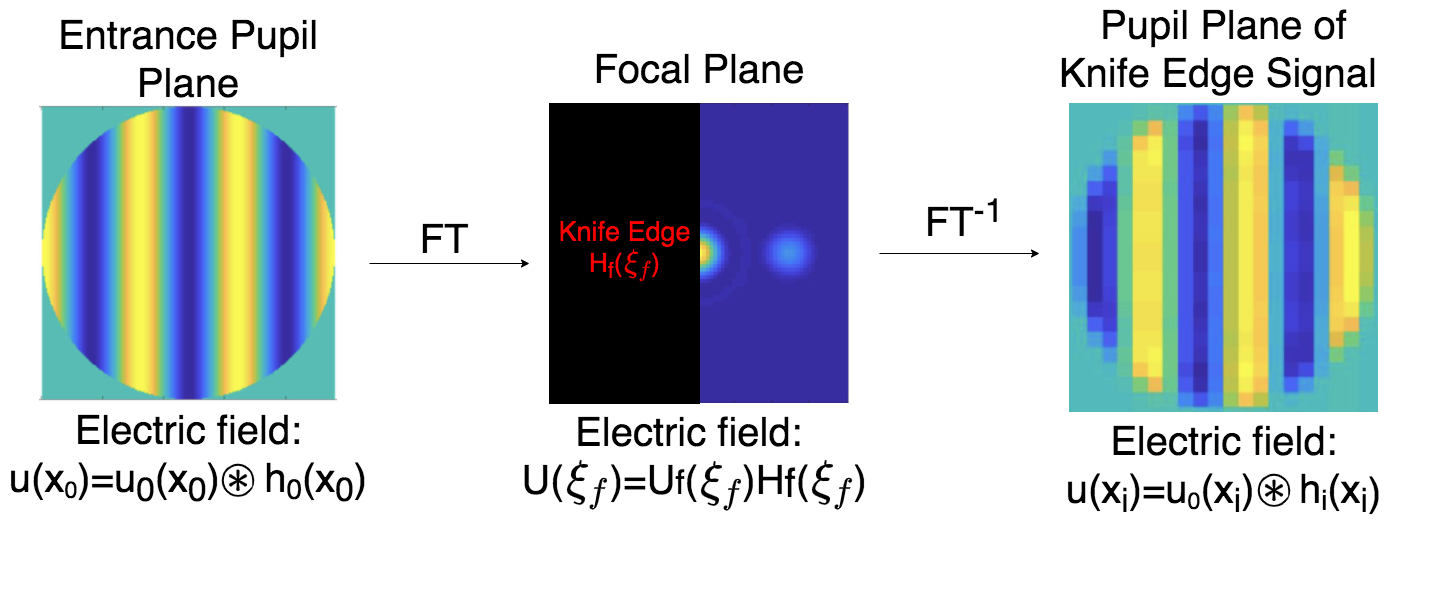
\includegraphics[width=0.9\textwidth]{Chapter Materials/Chapter Two Materials/DerivationFlow.png}
     \caption{Diagram of the steps taken in the derivation. The entrance pupil with electric field $u_0(x_0)$ is Fourier transformed to the focal plane. At the focal plane the knife edge by multiplying the binary mask function of the knife edge, $H_f(\xi_f)$, by the Fourier transform of the electric field in the entrance pupil. An inverse Fourier transform taken to return to the pupil plane where the pyramid signal is detected.}
     \label{fig:derivationFlow}
 \end{figure}
 
 


% To start, we define some terms used in the derivation. 

% \begin{center}
%     \begin{tabular}{ | l |p{12cm}|}
%     \hline
%     $u_0(x_0)$ & Complex wavefront at the "phase object". This could be the surface of a mirror under testing, but for our application it is the phase errors in the pupil caused by atmospheric turbulence. \\ \hline
%     $u_i(x_i)$ & Complex wavefront at the image plane. For the pyrmaid wavefront sensor the image plane is the pupil plane. \\ \hline
%     $h(x_i)$ & The impulse response of the system. \\ \hline
%     $m(x)$ & The equation of phase error to be measured. $u(x)=exp(-2\pi i m(x))$  \\ \hline
%     $p(x_i )$ & The intensity pattern at the image plane due to the diffraction of the electric field with the knife-edge \\ \hline
%     \end{tabular}
% \end{center}

To start we define the electric field in the entrance pupil as $u_0(x_0)$. We take the Fourier transform the of the electric field to get to the focal plane, where we will apply the knife-edge. The Fourier transform is here defined as,

\begin{equation}
    \mathcal{F}\{\xi_x\}=\frac{1}{2\pi}\int_{-\infty}^\infty e^{-i x \xi_x} f(x) dx
    \label{FourierT}
\end{equation}

\noindent where $\xi_x$ is the spatial frequency corresponding to the spatial coordinate $x$. $\mathcal{F}\{\cdot\}$ denotes the Fourier transform operator, and  $\mathcal{F}^{-1}\{\cdot\}$ will denote its inverse. The equation of the electric field in the focal plane, $U(\xi_f)$ is:

\begin{equation}
    U (\xi_f)=U_f(\xi_f)H_f(\xi_f)
    \label{FT}
\end{equation}

\noindent where,
% We now multiply the transmission function of the knife edge, $H(\xi_x)$. In this derivation we assume that the knife edge is like a step function, the transmission of light is 1 until the edge of the knife edge is reached and then drops to zero. We assume for simplicity that the aperture is infinite, but that the knife edge eclipses half of it. After multiplication, the Fourier transform of equation must be taken again to calculate the electric field in the pupil plane. We write out the step function in terms of the sign function $sgn(\xi_x)$, in order to calculate the Fourier Transform easily. The transfer function of the knife edge is given by the following equation.
\[ 
H_f(\xi_f)= 1/2+1/2\mbox{sgn}(\xi_f) \left\{
\begin{array}{ll}
      1 \: for \: \xi_f >0\\
      0 \: for \: \xi_f <0\\
      
\end{array} 
\right. 
\]

\noindent is the binary mask function of the knife edge, and $U_f(\xi_f)$ is the Fourier transform of $u_0(x_0)$. Taking the inverse Fourier transform brings us to the conjugate pupil plane. The inverse Fourier transform of $H_f(\xi_f)$ is

% \begin{equation}
%      FT^{-1}[H(\xi_x)]=\frac{1}{2\pi}\int_{-\infty}^\infty e^{ i x \xi_x} ( \frac{1}{2}+\frac{1}{2}sgn(\xi_x)) d\xi_x \\
%  =\frac{1}{2}\delta(-x)+\frac{i}{2\pi}(\frac{1}{x})
% \label{delta}
% \end{equation}

\begin{equation}
    h_i(x_i)= \mathcal{F}^{-1}[H_f(\xi_f)] =
    % \frac{1}{2\pi} \int_{-\infty}^\infty e^{ i x \xi_f}
    % \left(
    %     \frac{1}{2} + \frac{1}{2} \mathrm{sgn}(\xi_f)
    % \right) d\xi_f
    % = 
    \frac{1}{2} \delta(-x_i) + \frac{i}{2\pi} \left(\frac{1}{x_i}\right)
\label{delta}
\end{equation}


%  = \frac{1}{2} \frac{1}{2\pi} \int_{-\infty}^\infty e^{- i x \xi_x}d\xi_x+\frac{1}{2} \frac{1}{2\pi}\int_{-\infty}^\infty e^{- i x \xi_x}sgn(\xi_x) d\xi_x
% \end{align*}

% We make use of the property of the delta function to solve for the Fourier Transform of $\frac{1}{2}$:

% \begin{equation}
%     \delta(x)=\frac{1}{2\pi}\int_{-\infty}^\infty e^{ i x \xi_x}d\xi_x
% \end{equation}

% which leads to,
    
% \begin{equation}
%     \frac{1}{2}\delta(x)=\frac{1}{2}\frac{1}{2\pi}\int_{-\infty}^\infty e^{ i x \xi_x}d\xi_x 
% \end{equation}

% where $\frac{1}{2}\delta(x)$ is the Fourier Transform of $\frac{1}{2}$. To solve for the Fourier transform of $\frac{1}{2} sgn(\xi_x)$ function, we use the derivative property.

% \begin{equation}
%   FT[\frac{d g(x)}{dx}]=i2\pi \xi_x G(\xi_x)
%   \label{derivativeProp}
% \end{equation}

% where the derivative of $\frac{1}{2} sgn(\xi_x)$ is $\delta(\xi_x)$. Plugging this into Equation~\ref{derivativeProp}, gives the result,
% \begin{equation}
%   FT[\frac{d sgn(\xi_x)}{d\xi_x}]=FT[\delta{\xi_x}]=1=2\pi i x G(x).
% \end{equation}

% Solving for $G(x)$,
% \begin{equation}
%  G(x)=\frac{1}{i2\pi x}.
% \end{equation}

% Now we can sum our answers to get the Fourier Transform of a step function.

% \begin{equation}
%  FT[step(\xi_x)]=\frac{1}{i2\pi x_i}+\frac{1}{2}\delta(x_i)
%  \label{knifeedge}
% \end{equation}

We take the results of Equation~\ref{delta} and convolve it with $u_0(x_i)$, which is the Fourier transform of $U_f(\xi_f)$ in Equation~\ref{FT}, to get the electric field at the pupil plane, $u(x_i)$. The resulting equation is Equation 5a from Wilson.\citep{wilson1975wavefront}


% \begin{equation}
%   u_i(x_i)= u_0(x_0) \circledast \frac{i}{2\pi x_i}+\frac{1}{2}\delta(-x_i) 
%  = \int_{-\infty}^\infty u_0(x')[\frac{1}{2}\delta(x'-x_i)+\frac{i}{2\pi}\frac{1}{x_i-x'}]dx' 
% \end{equation}
%  \begin{equation}
%       u_i(x_i) =\frac{1}{2}u_0(x_i)+\frac{i}{2\pi}\int_{-\infty}^\infty \frac{u_0(x')dx'}{x_i-x'}
%       \label{KEconv}
%  \end{equation}

\begin{equation}
    u(x_i)= u_0(x_i) \circledast \left(
        \frac{i}{2\pi x_i}+\frac{1}{2}\delta(-x_i)
    \right)
    =
    \int_{-\infty}^\infty
    u_0(x') \left[
        \frac{1}{2}\delta(x'-x_i)+\frac{i}{2\pi}\frac{1}{x_i-x'}
    \right] dx' 
    \label{KEconv}
\end{equation}

The first modification to Equation~\ref{KEconv} by Wilson and Katzoff is to assume that the pupil has a finite aperture, resulting in the integral limits of -1 to 1. The following equations are equations 6 through 9 in Wilson's paper \citep{wilson1975wavefront}. For a perfect wavefront we assume $u_0 (x_i )=1$.  Wilson and Katzoff define $m(x)$ as the local mirror error in half-wavelengths, but for our application it would be the phase errors caused by atmospheric turbulence. Assuming an electric field with some phase error $m(x)$ we first expand the electric field as a Taylor series as follows,
\begin{equation}
    u_0 (x_i )=e^{(-2\pi i m(x_i ))}=1-2\pi i m(x_i )-2\pi^2*m^2 (x_i )+...
    \label{taylorexp}
\end{equation}
\noindent and disregard all higher order terms. Substituting Equation~\ref{taylorexp} into Equation~\ref{KEconv} and simplifying gives:

% \begin{equation}
%     2\pi*u_i (x_i )=\pi[1-2\pi^2 m^2 (x_i )+2\int_{-1}^1\frac{m(x')}{x'-x_i} dx']
% +i[-2\pi^2 m(x_i)+\int_{-1}^1\frac{dx'}{x'-x_i}-2\pi^2\int_{-1}^1\frac{m^2(x')}{x'-x_i}dx']
% \end{equation}
\begin{multline}
    2\pi u(x_i ) = 
    \pi 
    \left[ 
        1-2\pi^2 m^2 (x_i )+2\int_{-1}^1 \frac{m(x')}{x'-x_i} dx'
    \right] \\
    +   i \left[
        -2\pi^2 m(x_i)+\int_{-1}^1\frac{dx'}{x'-x_i}
        -
        2\pi^2\int_{-1}^1\frac{m^2(x')}{x'-x_i}dx'
    \right]
\end{multline}



The intensity in the image plane is the modulus squared of this expression, of which we keep only the linear terms:

% As a side note the integral:$\int_{-1}^1\frac{dx'}{x'-x_i}$ is equal to $ln(\frac{1-x}{1+x})$.

% \begin{equation}
%     I(x_i)=\pi^2 + \ln^2(\frac{1-x}{1+x})+4\pi^2\int_{-1}^1\frac{m(x')}{x'-x_i} dx'-4\pi^2 m(x_i)\ln(\frac{1-x}{1+x})
% \end{equation}
\begin{equation}
    I(x_i) = \pi^2 + \ln^2 \left(
        \frac{1-x_i}{1+x_i}
    \right)
    +
    4 \pi^2 \int_{-1}^1 \frac{m(x')}{x'-x_i} dx'
    -
    4\pi^2 m(x_i) \ln\left(
        \frac{1-x_i}{1+x_i}
    \right)
\end{equation}

The result contains two constant terms, which represent the intensity response $I_r(x_i )$, which is the reference intensity pattern resulting from a perfect wavefront propagated through the optical system. This can be subtracted out. The other two terms are dependent on the shape of the wavefront error. After subtracting  $I_r (x_i )$ and dividing by $4\pi^2$ we are left with the intensity pattern due to a pure phase error $I_p(x_i)$:

% \begin{equation}
%     p(x_i)=\frac{I(x_i)-I_0(x_i)}{4\pi^2}\int_{-1}^1\frac{m(x')}{x'-x_i} dx'-m(x_i)\ln(\frac{1-x}{1+x}).
% \end{equation}

\begin{equation}
    I_p(x_i) = \left(\frac{I(x_i) - I_r(x_i)}{4\pi^2}\right)=
     PV \int_{-1}^1 \frac{m(x')-m(x_i)}{x'-x_i}dx'
\end{equation}    
    % \int_{-1}^1\frac{m(x')}{x'-x_i} dx'
    % -
    % m(x_i)\int_{-1}^1\frac{dx'}{x'-x_i} 


% Collecting all constant terms into $C$, we can combine the two terms above into a single equation.
% \begin{equation}
%     I_p(x_i)=C \left( PV \int_{-1}^1 \frac{m(x')-m(x_i)}{x'-x_i}dx'\right)
% \end{equation}

In this equation $PV$ stands for the principal value. The $PV$ is used to evaluate integrals that have a discontinuity, in our case this is when $x_i=x'$ \citep{johansson1999hilbert}. This is the result found by \cite{linfoot1948theory}, and is the equation currently used to describe the operation of the PWFS  \citep{verinaud2004nature}. In high contrast imaging we are interested in the effect of phase errors at different spatial frequencies as these correspond to contrast at specific locations in the post-coronagraphic focal plane. \cite{katzoff1971quantitative} showed that this equation accurately predicts the intensity pattern from phase errors that are described by a power series, $x^{N}$, but his solution to the expected intensity pattern due to phase errors in the form of sines and cosines does not match the signal from the PWFS. To find the response of a knife edge to an error of the form $\cos(nx)$, where $n$ is the spatial frequency, we need to modify the above derivation. In this derivation we assume an infinite aperture approximation, and take the integral from $-\infty$ to $\infty$ instead of from -1 to 1. We start at Equation~\ref{taylorexp}, and consider only the linear component and substitute into Equation~\ref{KEconv}.  The electric field at the entrance aperture is now: 


\begin{equation}
    u_0(x_i )=\exp(-2\pi i m(x_i ))=1-2\pi i m(x_i).
    \label{EF}
\end{equation}

We substitute Equation~\ref{EF} into Equation~\ref{KEconv} to find the electric field in the pupil plane $u(x_i)$, which yields:

\begin{equation}
    u(x_i)= \frac{1}{2}(1-2\pi i m(x_i))+\frac{i}{2\pi}\int_{-\infty}^\infty \frac{(1-2\pi i m(x'))dx'}{x_i-x'}
    \label{HT}
\end{equation}

Expanding the integral, we have:
\begin{equation}
    u(x_i)= \frac{1}{2}(1-2\pi i m(x_i))+\frac{i}{2\pi}\int_{-\infty}^\infty \frac{dx'}{x_i-x'}+\int_{-\infty}^\infty \frac{ m(x')dx'}{x_i-x'}
\end{equation}

\noindent where the integrals are now in the form of a Hilbert transform \citep{villa2014foucault}. The Hilbert transform is defined as:

\begin{equation}
    H(y(t))=\frac{-1}{\pi} PV\int_{\infty}^{\infty} \frac{y(t') dt'}{t'-t}
\end{equation}

\noindent which has the property that the Hilbert transform of a constant is 0 \citep{poularikas2018handbook}. When the wavefront error is given by $m(x)=\cos(nx)$, Equation~\ref{HT} becomes, 


\begin{equation}
    u(x_i)= \frac{1}{2}(1-2\pi i \cos(nx_i))+\int_{-\infty}^\infty \frac{ \cos(nx')dx'}{x_i-x'}
\end{equation}

To get the integral in the form of a Hilbert transform we multiply by $\frac{\pi}{\pi}$. The Hilbert transform of $H(\cos(nx))=\cos(nx+\frac{\pi}{2})=-\sin(nx)$.

\begin{equation}
\int_{-\infty}^\infty \frac{ \cos(nx')dx'}{x_i-x'}=\pi*[\frac{1}{\pi}\int_{-\infty}^\infty \frac{ \cos(nx')dx'}{x_i-x'}]=-\pi \sin(nx_i)
\end{equation}

The equation for the electric field in the pupil plane of the knife edge signal is,

\begin{equation}
   u(x_i)= \frac{1}{2}-i \pi \cos(nx_i) -\pi \sin(nx_i)
   \label{derivationResult}
\end{equation}

\noindent and we can now take the modulus squared to get the intensity.

\begin{equation}
    I(x_i)=\frac{1}{4}+\pi^2-\pi \sin(nx_i)
    \label{equationIntensityResult}
\end{equation}

Subtracting the constant terms which represent the intensity response $I_r (x_i )$ to a perfect wavefront, gives the intensity pattern due only to phase errors. In this derivation we find an intensity pattern that is proportional to $-\sin(nx)$ resulting from a phase error of the form $\cos(nx)$. In the next section we demonstrate that this is the expected response.

\subsection{Verification}

The approximations we used to derive Equation~\ref{derivationResult} are supported by our simulation of the response of a PWFS to a cosine phase error. Using OOMAO we apply a Fourier mode as a phase error in the pupil plane, propagate through the pyramid onto the detector, and examine the resulting intensity pattern on the detector as well as the calculated slopes. The PWFSs are under $5 \frac{\lambda}{D}$ modulation to insure that the pyramid response is linear for the amplitude of Fourier mode applied, and we are not including any noise. We apply a Fourier mode phase error that is in the form of $\cos(3x)$ in the $x$-direction. The phase error in radians is shown in Figure \ref{fig:CosinePhaseDiagram}, where Figure \ref{fig:CosinePhaseDiagram}.A is the $\cos(3x)$ phase error, and Figure \ref{fig:CosinePhaseDiagram}.B is a cross section of the center function in the $x$-direction. We compare the resulting intensity patterns to our prediction in Equation~\ref{equationIntensityResult}. For an intensity pattern of the form $\cos(3x)$ shown in Figure \ref{fig:MathPredicions}.A, we would expect an intensity pattern in a pyramid pupil to be $1/4+\pi^2-\pi \sin(3x)$ displayed in Figure \ref{fig:MathPredicions}.B. After subtracting off constant terms we scale the amplitude of the signal such that the maximum value is 1, to compare the resulting pyramid signal is $-sin(3x)$ plotted in Figure \ref{fig:MathPredicions}.C.


\begin{figure}
    \centering
    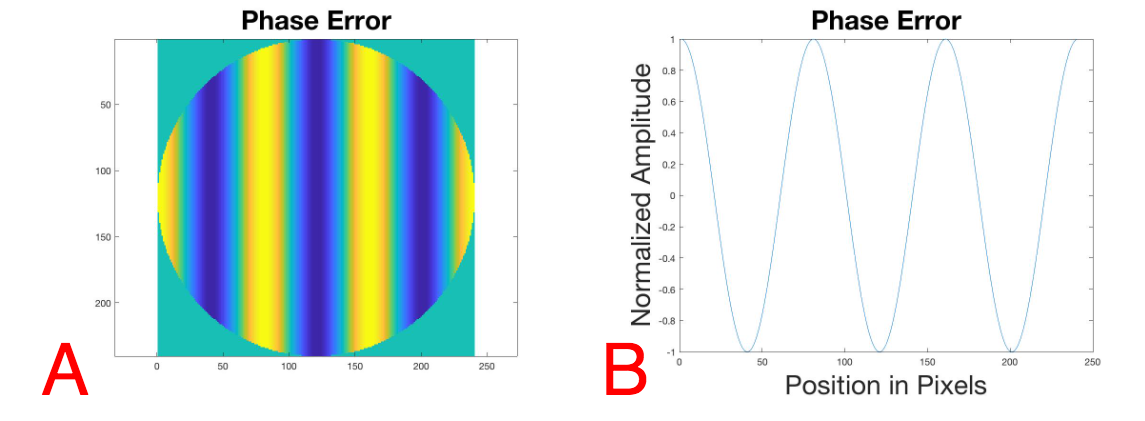
\includegraphics[width=0.8\textwidth]{Chapter Materials/Chapter Two Materials/CosinePhaseDiagram.png}
    \caption{A. Applied cosine phase error in radians in pupil plane to be propagated through the PWFS. B. Scaled cross section of the phase error.}
    \label{fig:CosinePhaseDiagram}
\end{figure}

\begin{figure}
    \centering
    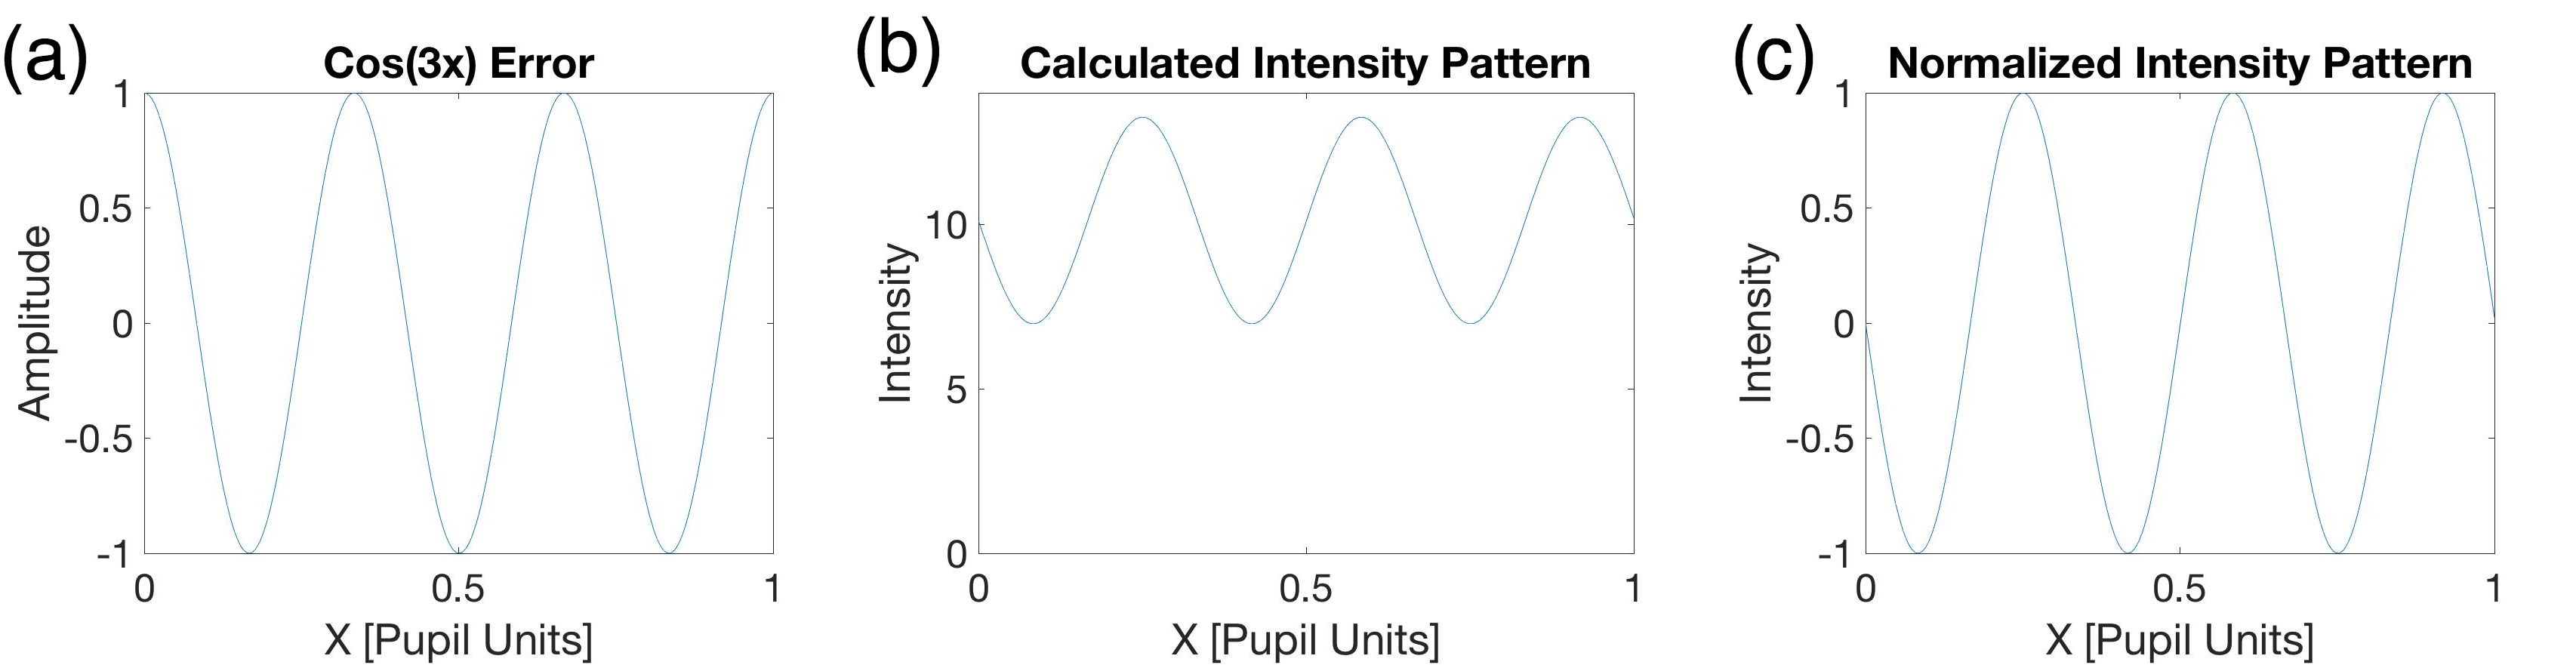
\includegraphics[width=1\textwidth]{Chapter Materials/Chapter Two Materials/MathPredictions.png}
    \caption{Predictions from the Foucault derivation. A. The applied $\cos(3x)$ phase error. B. The intensity pattern predicted for a single pupil. C. The expected pyramid signal after subtracting off constant terms and scaling.}
    \label{fig:MathPredicions}
\end{figure}

The resulting intensity patterns from the 3PWFS and 4PWFS are shown in Figure \ref{fig:IntensityPatternsDiagram} A and B. In Figure \ref{fig:IntensityPatternsDiagram} C and D we take a cross section from one of the pupils from each wavefront sensor and scale the signal. We then plot this against the predicted scaled intensity pattern. We find that the mathematical prediction is a good match for the measured intensity pattern inside the pupil of a modulated pyramid when the signal is linear. 


\begin{figure}
    \centering
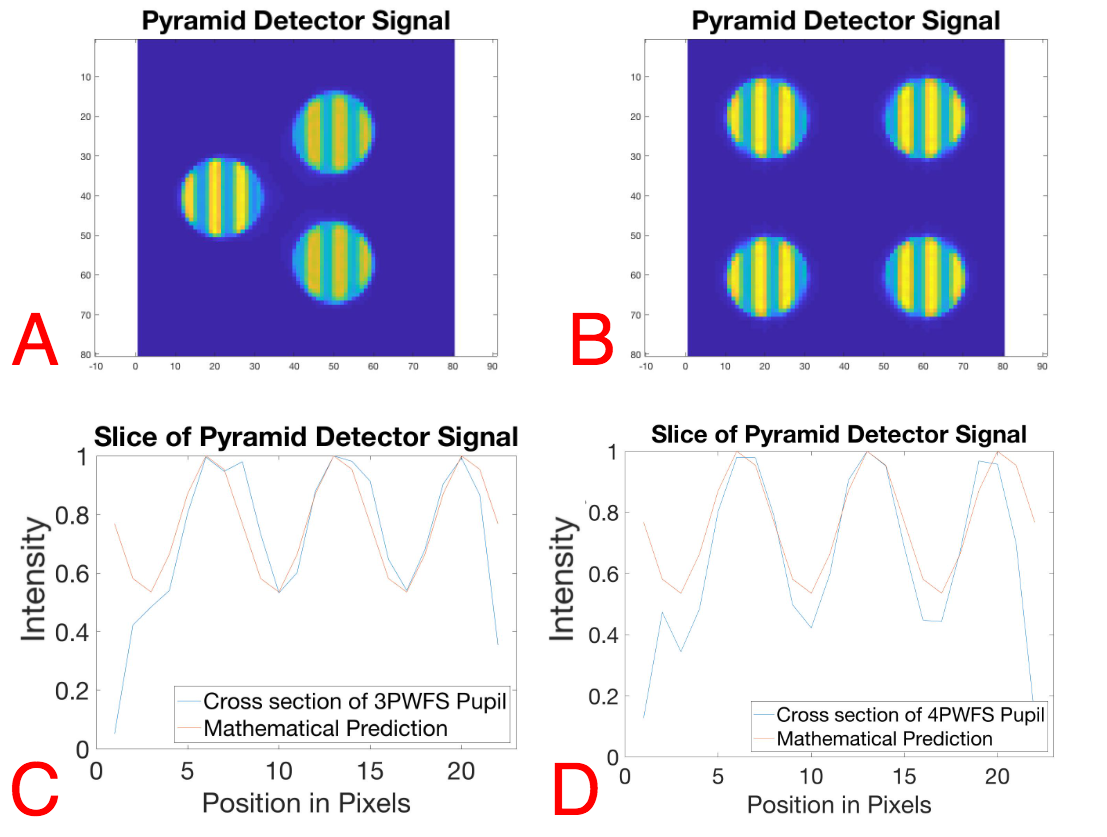
\includegraphics[width=0.8\textwidth]{Chapter Materials/Chapter Two Materials/IntensityPatternsDiagram.png}
    \caption{Resulting intensity patterns on the PWFS detector from A. the 3PWFS, and B. the 4PWFS. Figures C. and D. are cross section of the intensity pattern plotted against the mathematical prediction. For C. The cross section was taken from center of the middle-left pupil. For D. The cross section was taken from the center of the top two pupils.}
    \label{fig:IntensityPatternsDiagram}
\end{figure}

To gain further clarity we use the Slopes Maps equation that subtracts off the constant intensity and turns the signal into a pure X and Y measurement of phase. The Slopes Maps naturally subtracts the flat wavefront response and in that way is self-referencing.  More details on the Slopes calculation  for the 3PWFS is in Section~\ref{Slopes}. The Slopes Maps for the 3PWFS and the 4PWFS are shown in Figure \ref{fig:SlopesMapDiagram}, as well as the cross sections that are indeed a $-\sin(nx)$ function. 

\begin{figure}
    \centering
    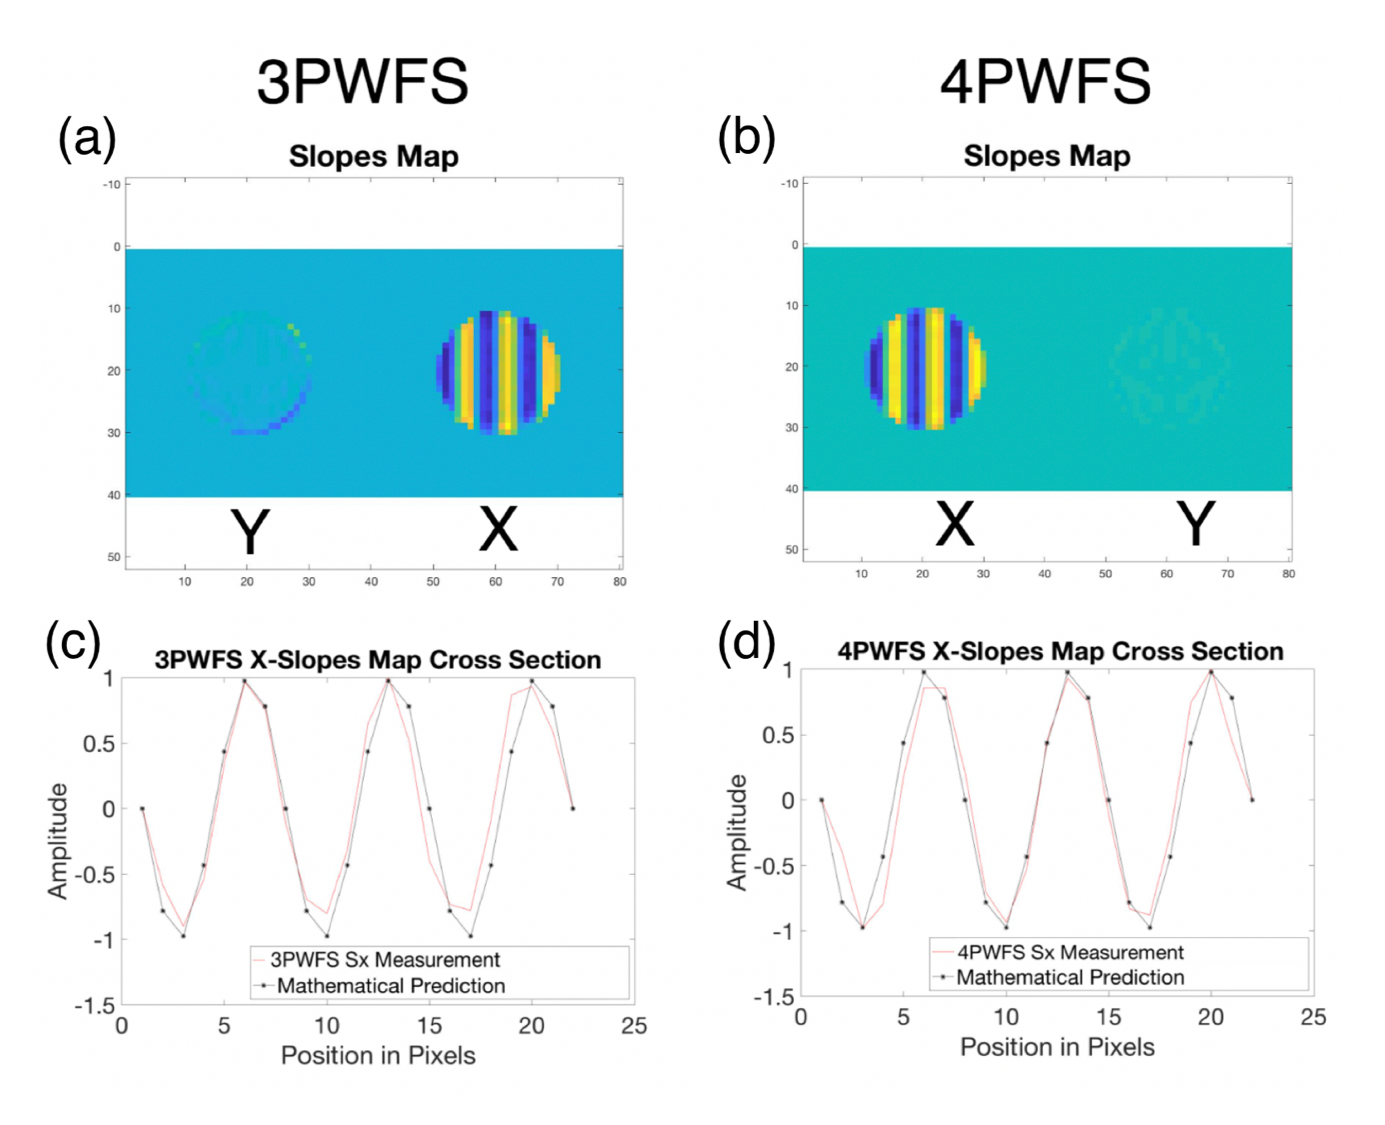
\includegraphics[width=0.9\textwidth]{Chapter Materials/Chapter Two Materials/SlopesandSlices.png}
    \caption{A. and B. Calculated slopes from the pyramid pupils. C. and D. Cross section of the Slopes plotted against the predicted signal. }
    \label{fig:SlopesMapDiagram}
\end{figure}

The previous simulations were performed with $5\lambda/D$ modulation. We can consider the 0 modulation case, which is a more direct relation to the results from the derivation. The unmodulated PWFS signal is more nonlinear than the modulated pyramid and therefore the fit between the prediction and the measured signal will be poor. In the case of the Slopes Maps signal, we found in simulation that the self-referencing is degraded from a nonlinear signal, and to return to a closer estimate of the signal the flat wavefront reference signal should be subtracted off. The fit worsens for the Slopes Maps without reference subtraction when there is a misregistration of the pupils, as will always be the case for the 3PWFS. For the 3PWFS subtracting off a reference improved the mean square error of the fit of simulation to derivation by about a factor of two, from 0.216 without subtraction, to 0.098 in the reference subtracted case. Figure \ref{fig:Mod0} summarizes the findings from the simulations with 0 modulation. Figure \ref{fig:Mod0}.A and \ref{fig:Mod0}.B are the detector signal of the 4PWFS and 3PWFS to the $\cos(3x)$ phase error. Figure \ref{fig:Mod0}.C and \ref{fig:Mod0}.D are a cross section of the scaled Slopes Maps plotted against the predicted signal. Figure \ref{fig:Mod0}.E and Figure \ref{fig:Mod0}. F are cross sections of the Slopes Maps with the reference signal subtracted.

\begin{figure}
    \centering
    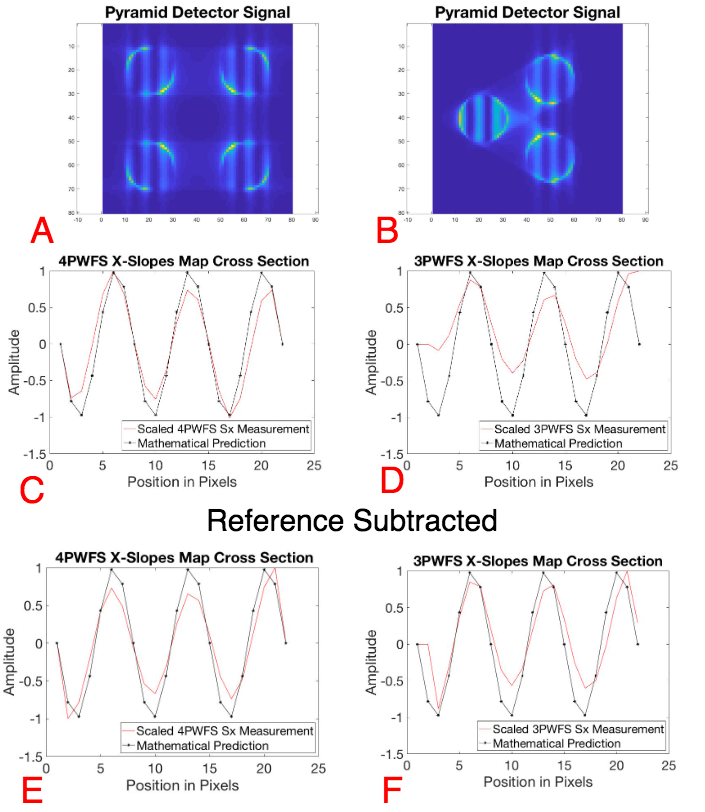
\includegraphics[width=0.9\textwidth]{Chapter Materials/Chapter Two Materials/Mod0PredictionVsSIm.png}
    \caption{A. and B. The wavefront sensor detector signals. C. and D. cross section of the wavefront sensor Slopes Maps plotted against the prediction. E. and F. the cross section of the Slopes Maps with the reference signal subtracted.}
    \label{fig:Mod0}
\end{figure}

The diffraction theory of the Foucault test predicts an intensity pattern that is the Hilbert transform of the wavefront phase. The result is an intensity pattern that is related to the wavefront derivative, but is not quite the derivative. In the case of a derivative wavefront sensor such as the Shack-Hartmann, the operation of the wavefront sensor on the phase to signal measurement is $\frac{d}{dx}\cos(nx)=-n\sin(nx)$. In the case of the pyramid the reference subtracted result is  $\frac{d}{dx}\cos(nx)=-\sin(nx)$, which is similar to the derivative wavefront sensor but without the scaling by spatial frequency. The result is that the knife edge and therefore the unmodulated pyramid sensitivity does not depend on spatial frequency as found in previous work by \cite{guyon2005}, because all spatial frequencies will produce an equally strong signal. In the Shack-Hartmann case the strength of the signal scales linearly with spatial frequency.


\section{3PWFS Slopes Maps}\label{Slopes}

\subsection{Derivation}\label{SlopesDerivation}

The Slopes Maps technique was derived for the 4PWFS using the same intensity centroid calculation as a Shack-Hartmann wavefront sensor. The Shack-Hartmann uses a quad-cell intensity calculation to track the movement of spots to calculate the X and Y gradient of the wavefront phase in post-processing. In the geometric optics approximation the PWFS acts as a slope sensor, and the Slopes Maps calculates the wavefront gradients in a similar way to the Shack-Hartmann. In the diffractive optics derivation, the wavefront slopes are calculated by the diffraction of the pyramid edges and encoded directly into the intensity pattern. We do not need to perform a Slopes Maps calculation for the pyramid signal because we are directly measuring a function that is related to the gradient phase error, but it is still beneficial to do so. The Slopes Maps is the natural recombination of the pyramid signals that subtracts off the constant Intensity pattern, so a reference image is not required. In a closed loop system the wavefront signal is driven towards  zero slope which arises when the PSF is centered on the pyramid tip with no phase errors. The Slopes Maps technique suffers from misalignments of the pyramid pupils; any misregistration in the sampling of the pupils with respect to each other results in a loss of performance. 

The Slopes Maps for the 4PWFS is already known. In previous work by Costa, a Slopes Map calculation for the 3PWFS was derived assuming a geometric optics approximation of the PWFS as a derivative wavefront sensor in the modulation regime \citep{buchler2004development}. In this paper we introduce a new Slope Maps method to handling the 3PWFS signals, which is derived using the intensity centroid of an equilateral triangle.

To calculate the Slopes Maps equations for the 3PWFS, we start from the same assumptions used for the 4PWFS. We assume that the maximum sensitivity of the sensor occurs when the PSF is centered at the tip of the four pyramid edges. We seek a Slopes Maps equation that drives the wavefront to zero slope, resulting in uniform intensity in the re-imaged pupils. To derive the centroid equation for the 3PWFS we start with an equilateral triangle, shown in Figure \ref{fig:triCentFig}. The center of the triangle is at the origin of a Cartesian coordinate system, and the vertices of the triangle are all an equal distance from the origin. The blue circles represent the layout of the pupils on the PWFS detector, and $I_1$ corresponds to $(x_1, y_1)$, etc. Solving for the coordinates $(x_1,y_1),(x_2,y_2), (x_3,y_3)$ gives the weights in the $S_x$ and $S_y$ Slopes Maps. 

% We can see in Equation~\ref{4PWFSslopes} that when the pixel values are equal the value of the Slopes are zero.

\begin{figure}
\begin{center}
\begin{tabular}{c}
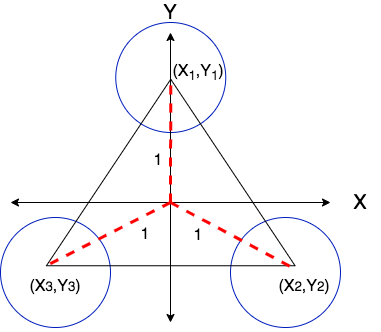
\includegraphics[height=5.5cm]{Chapter Materials/Chapter Two Materials/3PWFSslopesMap.png}
\end{tabular}
\end{center}
\caption 
{ \label{fig:triCentFig}
Equilateral triangle with the center at the origin. Solving for the coordinates of the vertex points gives the weights for the pixel Intensities used in the Slopes Maps calculation. The blue circles represent the layout of the pupils on the detector. } 
\end{figure} 

For the 3PWFS we find that the $S_x$ and $S_y$ Slopes Maps are,
% \begin{equation}
%     S_x=\frac{\frac{\sqrt{3}}{2}I_2-\frac{\sqrt{3}}{2}I_3}{I_1+I_2+I_3}, \; \;
%     S_y=\frac{I_1-\frac{1}{2}I_2-\frac{1}{2}I_3}{I_1+I_2+I_3}
%     \label{3PWFSslopes}
% \end{equation}

\begin{eqnarray}
    S_x=\frac{\frac{\sqrt{3}}{2}I_2-\frac{\sqrt{3}}{2}I_3}{I_1+I_2+I_3} \label{3PWFSslopes} \\
    S_y=\frac{I_1-\frac{1}{2}I_2-\frac{1}{2}I_3}{I_1+I_2+I_3} \nonumber
\end{eqnarray}

The $S_x$ slopes maps in this orientation depends only on the intensities from the $I_2$ and $I_3$ pupil pixels which act as a roof sensor. The result is that care must be taken to properly index the pupils when applying the Slopes Map equation. 
 
\subsection{Testbed Verification}
 
To test the validity of the Slopes Maps equation for the 3PWFS, and the Raw Intensity method we implemented these signal processing methods into a real closed adaptive optics system using the LOOPS testbed at the Laboratoire d'Astrophysique de Marseille.  The layout of the LOOPs testbed is detailed in Figure REF. The source for the LOOPs is a HeNe laser attenuated by a continuously variable gradient ND filter wheel. There are multiple paths through the loops testbed created by beamsplitters. Different branches can be blocked or passed to create modes where the testbed only uses flat mirrors to record a reference PSF, and to illuminate the deformable mirror and phase screen. The phase screen is a reflective and simulates a $D/r_0$ of about 28. The wind speed of the turbulence can be changed by speeding up or slowing down a stepper motor that rotates the phase screen. An ALPAO 69 actuator deformable mirror is used to for the closed loop correction. A phase screen applied on a spatial light modulator (SLM) is used to create the pyramid tip. The wavefront sensing camera is an OCAM$^2$K used in single pixel mode. Each pyramid pupil is 80 pixels in diameter. A full description of the LOOPS testbed can be found in  \cite{janin2019adaptive}. 

\begin{figure}
    \centering
    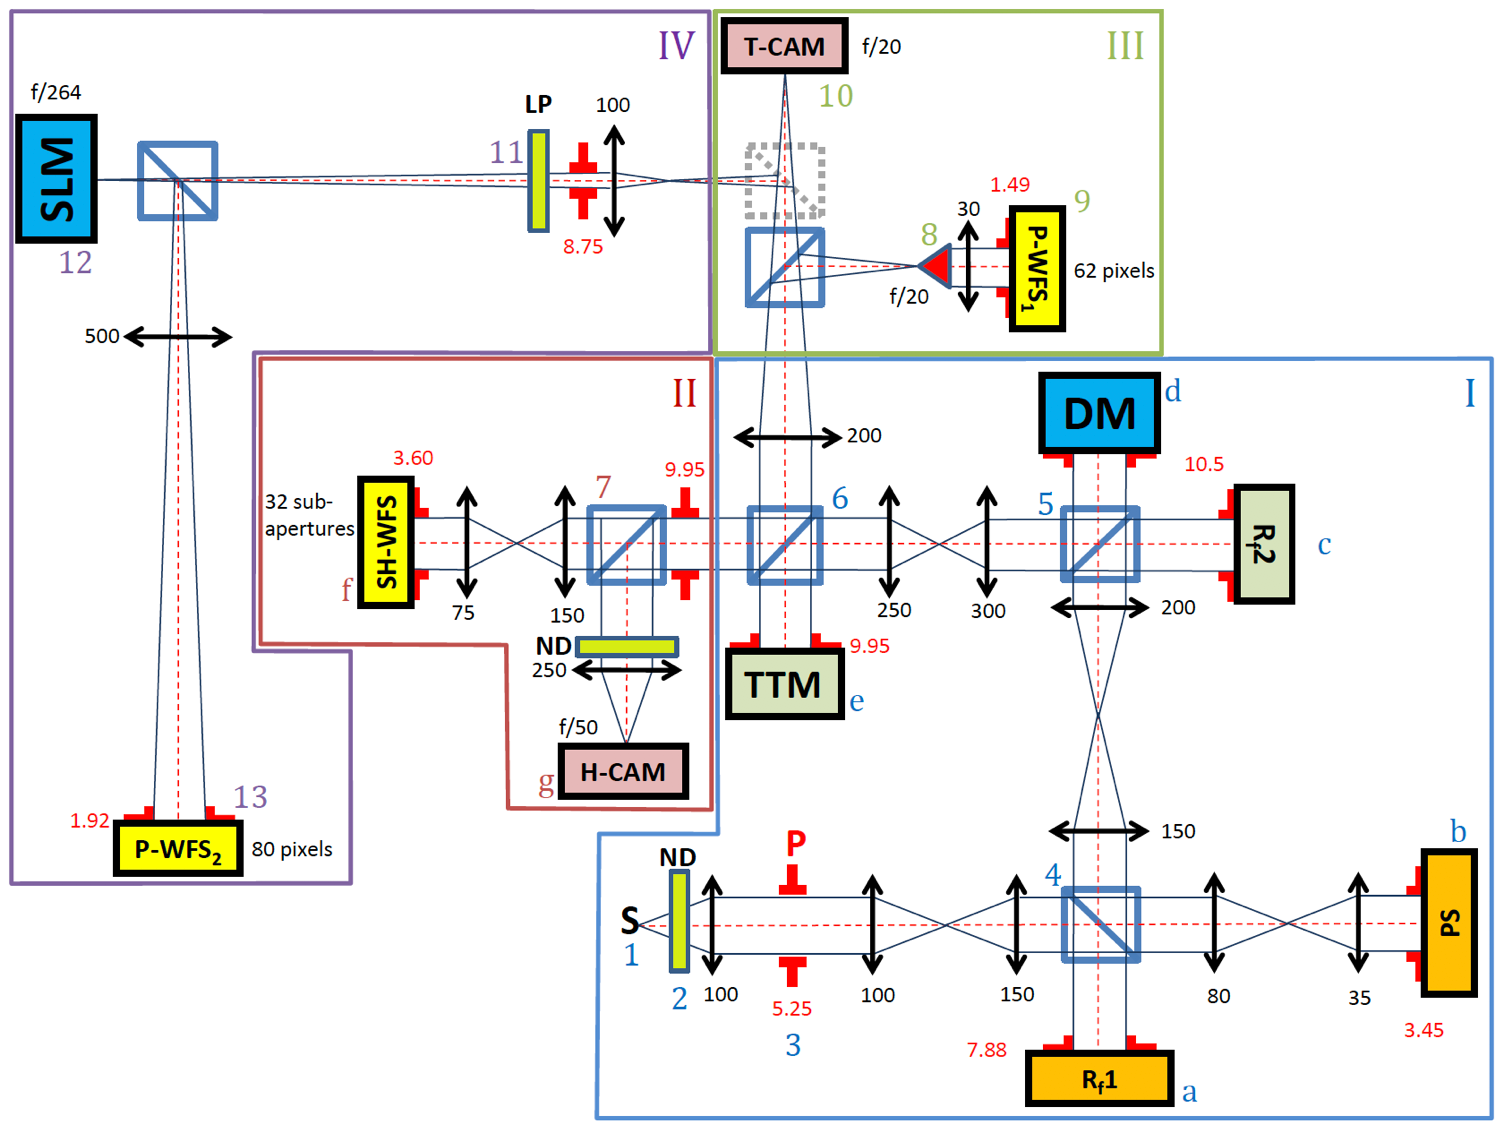
\includegraphics[width=0.8\textwidth]{Chapter Materials/Chapter Four Materials/LOOPSdiagram.png}
    \caption{Schematic of the LOOPS testbed. The pupil planes are marked in red. Light starts at the source marked S and propagates to the right to either the phase screen or a flat reference mirror. Next the light can be passed to either the deformable mirror or another flat mirror. For this experiment only the SLM was used to create the pyramid optics. The wavefront sensing camera (P-WFS$_2$) is an OCAM$^2$K camera with pupils 80 pixels in diameter \citep{janin2019adaptive}.}
    \label{fig:my_label}
\end{figure}


On the testbed a closed loop correction was achieved for both a 3PWFS and 4PWFS with reconstructors calculated from both the Raw Intensity and Slopes Maps signal handling techniques. The loop was run at 250Hz, with a modulation radius of 5 $\lambda/D$. In all cases a stable closed loop was obtained. Figure \ref{fig:LOOOPS} shows example images from the LOOPS test-bed of (A) the pyramid signal of the 3PWFS under turbulence in closed loop, (B) the pyramid signal of the 4PWFS under turbulence in closed loop, (C) the LOOPS PSF with no turbulence, and (D) the LOOPS PSF in closed loop with the 3PWFS using the Slopes Map technique. An experiment was performed to measure and compare Strehl between the wavefront sensor. The results of the experiment were inconclusive due to the lack of confidence in the consistency and optimization of measurements taken. The ALPAO deformable mirror was found to have significant drift and hysteresis resulting in the need to resharpen the PSF on the pyramid tip frequently. In addition due to the surface quality or the performance of the SLM, the pyramid pupils were not high quality. In the 4PWFS the edges of two of the pyramid pupils were blurry. One of the pupils on the 3PWFS suffered significantly from this affect. The effect on the quality of the wavefront reconstruction by each of the PWFS was not quantified. 

\begin{figure}
    \centering
    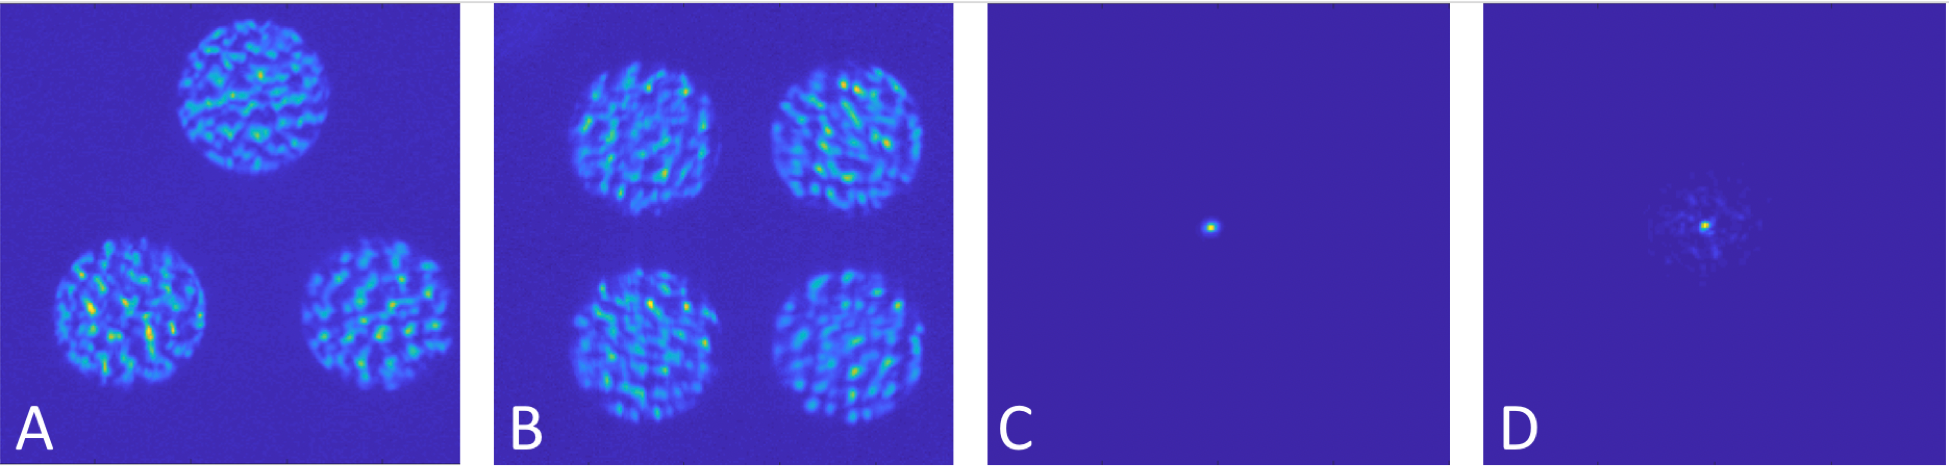
\includegraphics[width=0.8\textwidth]{Chapter Materials/Chapter Two Materials/LOOPS.png}
    \caption{Example images from the LOOPS test-bed of A) the pyramid signal of the 3PWFS under turbulence in closed loop, B) the pyramid signal of the 4PWFS under turbulence in closed loop, C) the LOOPS PSF with no turbulence, and D) the LOOPS PSF in closed loop with the 3PWFS using the Slopes Map technique.}
    \label{fig:LOOOPS}
\end{figure}

\section{The Reconstructor Matrix}

In the previous sections, we have derived what the expected signal is from the pyramid wavefront sensor, and how to process the signal to retain only the intensity pattern due to phase errors. We will now detail the processes of building a reconstructor matrix from wavefront sensor signals that allow us to reconstruct the wavefront error.
 
The wavefront sensor measures a signal $S$, which includes the signal processing discussed in Section \ref{PWFSintro}. The signal can be decomposed into a summation of modes from a basis set. The interaction matrix, $I$, is the bridge between the deformable mirror commands and the wavefront signals. The interaction matrix is calibrated by applying modes on the deformable mirror and recording the response from the wavefront sensor. The intensity measurements are unraveled from a 2D detector image into a 1D vector and stored as a column vector in the interaction matrix. We can use the interaction matrix to apply shapes on the deformable mirror by summing modes that are weighted by amplitudes stored in the amplitude matrix $A$. The interaction matrix and the amplitude matrix are related to the wavefront sensor signal by $S=IA$. In the AO case, we measure $S$, which is a $[M\times 1]$ matrix of wavefront sensor signals from aberrated starlight, and calibrate to find $I$ which is a $[M\times N]$ matrix. The dimension $M$ is the sampling of the wavefront measurement. For the Raw Intensity method $M$ is equal to the number of pixels in the pupils, and for Slopes Maps $M$ is equal to the sampling of both the $S_x$ and $S_y$ measurement. The dimension $N$ is the number of modes in the basis set used for wavefront reconstruction. To reconstruct the signal we need to find $A$, a $[N\times 1]$ matrix the corresponding amplitudes that will give us the right wavefront shape. We cannot compute the operation $A=I^{-1}S$, because $I$ is an $[M\times N]$ size matrix and not invertible. To find $A$, a pseudo-inverse of $I$ is calculated using singular value decomposition (SVD). The SVD of I is calculated by,

\begin{equation}
    SVD(I)=U\Sigma V^T
\end{equation}

\noindent where $U$ is a $[M\times M]$ matrix, $Sigma$ is an $[M\times N]$ matrix with singular values on the diagonal, and $V$ is a $[N\times N]$ matrix. We calculate the reconstructor matrix $R$ which is the pseudo-inverse of $I$ using $U$,$V$,and $\Sigma$.

\begin{equation}
   R=V\Sigma^{\dag}U^T
\end{equation}

The Reconstructor matrix R is a $[N\times M]$ sized matrix, and we calculate the vector of modal amplitudes using:

\begin{equation}
    A=RS
    \label{ReconEq}
\end{equation}

An additional matrix $C$ of size $[K\times N]$ giving the commands to drive the deformable mirror to shapes that are modes in the basis set is needed. The amplitude matrix $A$ scales this command matrix so that the proper amplitude of each mode is applied. The multiplication $V=CA$, where $V$ is a matrix of actuator positions gives a $[K\times 1]$ vector of the deformable mirror commands where $K$ is the total number of actuators used on the deformable mirror for wavefront control.  Reshaping the $[K\times 1]$ matrix into a $[\sqrt{K}\times \sqrt{K}]$ matrix gives the command for each actuator in the deformable mirror, where the deformable mirror is a square of $\sqrt{K}\times \sqrt{K}$ actuators.
\include{ch5HotellingObserver}
\include{ch6NullHypothesis}
\include{ch7FutureWork}

\renewcommand{\baselinestretch}{1}		% chaning the value
\small\normalsize						% switch size to make the value take

\bibliographystyle{uabibnat}  
\bibliography{report.bib}

\end{document}

